\documentclass[twoside]{book}

% Packages required by doxygen
\usepackage{fixltx2e}
\usepackage{calc}
\usepackage{doxygen}
\usepackage[export]{adjustbox} % also loads graphicx
\usepackage{graphicx}
\usepackage[utf8]{inputenc}
\usepackage{makeidx}
\usepackage{multicol}
\usepackage{multirow}
\PassOptionsToPackage{warn}{textcomp}
\usepackage{textcomp}
\usepackage[nointegrals]{wasysym}
\usepackage[table]{xcolor}

% Font selection
\usepackage[T1]{fontenc}
\usepackage[scaled=.90]{helvet}
\usepackage{courier}
\usepackage{amssymb}
\usepackage{sectsty}
\renewcommand{\familydefault}{\sfdefault}
\allsectionsfont{%
  \fontseries{bc}\selectfont%
  \color{darkgray}%
}
\renewcommand{\DoxyLabelFont}{%
  \fontseries{bc}\selectfont%
  \color{darkgray}%
}
\newcommand{\+}{\discretionary{\mbox{\scriptsize$\hookleftarrow$}}{}{}}

% Page & text layout
\usepackage{geometry}
\geometry{%
  a4paper,%
  top=2.5cm,%
  bottom=2.5cm,%
  left=2.5cm,%
  right=2.5cm%
}
\tolerance=750
\hfuzz=15pt
\hbadness=750
\setlength{\emergencystretch}{15pt}
\setlength{\parindent}{0cm}
\setlength{\parskip}{3ex plus 2ex minus 2ex}
\makeatletter
\renewcommand{\paragraph}{%
  \@startsection{paragraph}{4}{0ex}{-1.0ex}{1.0ex}{%
    \normalfont\normalsize\bfseries\SS@parafont%
  }%
}
\renewcommand{\subparagraph}{%
  \@startsection{subparagraph}{5}{0ex}{-1.0ex}{1.0ex}{%
    \normalfont\normalsize\bfseries\SS@subparafont%
  }%
}
\makeatother

% Headers & footers
\usepackage{fancyhdr}
\pagestyle{fancyplain}
\fancyhead[LE]{\fancyplain{}{\bfseries\thepage}}
\fancyhead[CE]{\fancyplain{}{}}
\fancyhead[RE]{\fancyplain{}{\bfseries\leftmark}}
\fancyhead[LO]{\fancyplain{}{\bfseries\rightmark}}
\fancyhead[CO]{\fancyplain{}{}}
\fancyhead[RO]{\fancyplain{}{\bfseries\thepage}}
\fancyfoot[LE]{\fancyplain{}{}}
\fancyfoot[CE]{\fancyplain{}{}}
\fancyfoot[RE]{\fancyplain{}{\bfseries\scriptsize Generated by Doxygen }}
\fancyfoot[LO]{\fancyplain{}{\bfseries\scriptsize Generated by Doxygen }}
\fancyfoot[CO]{\fancyplain{}{}}
\fancyfoot[RO]{\fancyplain{}{}}
\renewcommand{\footrulewidth}{0.4pt}
\renewcommand{\chaptermark}[1]{%
  \markboth{#1}{}%
}
\renewcommand{\sectionmark}[1]{%
  \markright{\thesection\ #1}%
}

% Indices & bibliography
\usepackage{natbib}
\usepackage[titles]{tocloft}
\setcounter{tocdepth}{3}
\setcounter{secnumdepth}{5}
\makeindex

% Hyperlinks (required, but should be loaded last)
\usepackage{ifpdf}
\ifpdf
  \usepackage[pdftex,pagebackref=true]{hyperref}
\else
  \usepackage[ps2pdf,pagebackref=true]{hyperref}
\fi
\hypersetup{%
  colorlinks=true,%
  linkcolor=blue,%
  citecolor=blue,%
  unicode%
}

% Custom commands
\newcommand{\clearemptydoublepage}{%
  \newpage{\pagestyle{empty}\cleardoublepage}%
}

\usepackage{caption}
\captionsetup{labelsep=space,justification=centering,font={bf},singlelinecheck=off,skip=4pt,position=top}

%===== C O N T E N T S =====

\begin{document}

% Titlepage & ToC
\hypersetup{pageanchor=false,
             bookmarksnumbered=true,
             pdfencoding=unicode
            }
\pagenumbering{roman}
\begin{titlepage}
\vspace*{7cm}
\begin{center}%
{\Large Naivik Robot \\[1ex]\large 0.\+1 }\\
\vspace*{1cm}
{\large Generated by Doxygen 1.8.11}\\
\end{center}
\end{titlepage}
\clearemptydoublepage
\tableofcontents
\clearemptydoublepage
\pagenumbering{arabic}
\hypersetup{pageanchor=true}

%--- Begin generated contents ---
\chapter{Hierarchical Index}
\section{Class Hierarchy}
This inheritance list is sorted roughly, but not completely, alphabetically\+:\begin{DoxyCompactList}
\item \contentsline{section}{Camera}{\pageref{classCamera}}{}
\item \contentsline{section}{Motion\+Controller}{\pageref{classMotionController}}{}
\item \contentsline{section}{Naivik}{\pageref{classNaivik}}{}
\item \contentsline{section}{Obstacle\+Detection}{\pageref{classObstacleDetection}}{}
\item Test\begin{DoxyCompactList}
\item \contentsline{section}{Motion\+Controller\+Test}{\pageref{classMotionControllerTest}}{}
\item \contentsline{section}{Naivik\+Test}{\pageref{classNaivikTest}}{}
\item \contentsline{section}{Obstacle\+Detection\+Test}{\pageref{classObstacleDetectionTest}}{}
\end{DoxyCompactList}
\item \contentsline{section}{Test\+Helper}{\pageref{classTestHelper}}{}
\end{DoxyCompactList}

\chapter{Class Index}
\section{Class List}
Here are the classes, structs, unions and interfaces with brief descriptions\+:\begin{DoxyCompactList}
\item\contentsline{section}{\hyperlink{classCamera}{Camera} \\*\hyperlink{classCamera}{Camera} class handles viewing and taking images in front of the robot }{\pageref{classCamera}}{}
\item\contentsline{section}{\hyperlink{classMotionController}{Motion\+Controller} \\*\hyperlink{classMotionController}{Motion\+Controller} class determine\textquotesingle{}s robot control actions. R\+OS doesn\textquotesingle{}t provide any controller, thus we need to design our own based on the requirement that we have }{\pageref{classMotionController}}{}
\item\contentsline{section}{\hyperlink{classMotionControllerTest}{Motion\+Controller\+Test} \\*\hyperlink{classMotionController}{Motion\+Controller} fixture class }{\pageref{classMotionControllerTest}}{}
\item\contentsline{section}{\hyperlink{classNaivik}{Naivik} \\*\hyperlink{classNaivik}{Naivik} class handles the camera and motion controller interactions of the robot }{\pageref{classNaivik}}{}
\item\contentsline{section}{\hyperlink{classNaivikTest}{Naivik\+Test} \\*\hyperlink{classNaivik}{Naivik} fixture class }{\pageref{classNaivikTest}}{}
\item\contentsline{section}{\hyperlink{classObstacleDetection}{Obstacle\+Detection} \\*\hyperlink{classObstacleDetection}{Obstacle\+Detection} class handles determining if the vehicle is going to collide using laser scans data }{\pageref{classObstacleDetection}}{}
\item\contentsline{section}{\hyperlink{classObstacleDetectionTest}{Obstacle\+Detection\+Test} \\*\hyperlink{classObstacleDetection}{Obstacle\+Detection} fixture class }{\pageref{classObstacleDetectionTest}}{}
\item\contentsline{section}{\hyperlink{classTestHelper}{Test\+Helper} \\*\hyperlink{classTestHelper}{Test\+Helper} class handles in testing the nodes publisher and subscriber }{\pageref{classTestHelper}}{}
\end{DoxyCompactList}

\chapter{File Index}
\section{File List}
Here is a list of all files with brief descriptions\+:\begin{DoxyCompactList}
\item\contentsline{section}{/home/ashishpatel/project/src/naivik\+\_\+robot/include/\hyperlink{camera_8hpp}{camera.\+hpp} \\*\hyperlink{classCamera}{Camera} class header file }{\pageref{camera_8hpp}}{}
\item\contentsline{section}{/home/ashishpatel/project/src/naivik\+\_\+robot/include/\hyperlink{motionController_8hpp}{motion\+Controller.\+hpp} \\*\hyperlink{classMotionController}{Motion\+Controller} class header file }{\pageref{motionController_8hpp}}{}
\item\contentsline{section}{/home/ashishpatel/project/src/naivik\+\_\+robot/include/\hyperlink{naivik_8hpp}{naivik.\+hpp} \\*\hyperlink{classNaivik}{Naivik} class header file }{\pageref{naivik_8hpp}}{}
\item\contentsline{section}{/home/ashishpatel/project/src/naivik\+\_\+robot/include/\hyperlink{obstacleDetection_8hpp}{obstacle\+Detection.\+hpp} \\*\hyperlink{classObstacleDetection}{Obstacle\+Detection} class header file }{\pageref{obstacleDetection_8hpp}}{}
\item\contentsline{section}{/home/ashishpatel/project/src/naivik\+\_\+robot/src/\hyperlink{camera_8cpp}{camera.\+cpp} \\*\hyperlink{classCamera}{Camera} class implementation file }{\pageref{camera_8cpp}}{}
\item\contentsline{section}{/home/ashishpatel/project/src/naivik\+\_\+robot/src/\hyperlink{motionController_8cpp}{motion\+Controller.\+cpp} }{\pageref{motionController_8cpp}}{}
\item\contentsline{section}{/home/ashishpatel/project/src/naivik\+\_\+robot/src/\hyperlink{naivik_8cpp}{naivik.\+cpp} \\*\hyperlink{classNaivik}{Naivik} class implementation file }{\pageref{naivik_8cpp}}{}
\item\contentsline{section}{/home/ashishpatel/project/src/naivik\+\_\+robot/src/\hyperlink{naivik__robot__node_8cpp}{naivik\+\_\+robot\+\_\+node.\+cpp} \\*R\+OS package entry point }{\pageref{naivik__robot__node_8cpp}}{}
\item\contentsline{section}{/home/ashishpatel/project/src/naivik\+\_\+robot/src/\hyperlink{obstacleDetection_8cpp}{obstacle\+Detection.\+cpp} \\*\hyperlink{classObstacleDetection}{Obstacle\+Detection} class header file }{\pageref{obstacleDetection_8cpp}}{}
\item\contentsline{section}{/home/ashishpatel/project/src/naivik\+\_\+robot/tests/\hyperlink{cameraTest_8cpp}{camera\+Test.\+cpp} \\*Test cases for \hyperlink{classCamera}{Camera} class }{\pageref{cameraTest_8cpp}}{}
\item\contentsline{section}{/home/ashishpatel/project/src/naivik\+\_\+robot/tests/\hyperlink{main_8cpp}{main.\+cpp} \\*This file is used to run all the unit tests for the developed package }{\pageref{main_8cpp}}{}
\item\contentsline{section}{/home/ashishpatel/project/src/naivik\+\_\+robot/tests/\hyperlink{motionControllerTest_8cpp}{motion\+Controller\+Test.\+cpp} \\*Test cases for \hyperlink{classMotionController}{Motion\+Controller} class }{\pageref{motionControllerTest_8cpp}}{}
\item\contentsline{section}{/home/ashishpatel/project/src/naivik\+\_\+robot/tests/\hyperlink{naivikTest_8cpp}{naivik\+Test.\+cpp} \\*Test cases for \hyperlink{classNaivik}{Naivik} class }{\pageref{naivikTest_8cpp}}{}
\item\contentsline{section}{/home/ashishpatel/project/src/naivik\+\_\+robot/tests/\hyperlink{obstacleDetectionTest_8cpp}{obstacle\+Detection\+Test.\+cpp} \\*Test cases for \hyperlink{classObstacleDetection}{Obstacle\+Detection} class }{\pageref{obstacleDetectionTest_8cpp}}{}
\item\contentsline{section}{/home/ashishpatel/project/src/naivik\+\_\+robot/tests/\hyperlink{testHelper_8cpp}{test\+Helper.\+cpp} \\*\hyperlink{classTestHelper}{Test\+Helper} implementation file }{\pageref{testHelper_8cpp}}{}
\item\contentsline{section}{/home/ashishpatel/project/src/naivik\+\_\+robot/tests/\hyperlink{testHelper_8hpp}{test\+Helper.\+hpp} \\*Header file for \hyperlink{classTestHelper}{Test\+Helper} class }{\pageref{testHelper_8hpp}}{}
\item\contentsline{section}{/home/ashishpatel/project/src/naivik\+\_\+robot/tests/\hyperlink{testNodes_8cpp}{test\+Nodes.\+cpp} }{\pageref{testNodes_8cpp}}{}
\item\contentsline{section}{/home/ashishpatel/project/src/naivik\+\_\+robot/tests/\hyperlink{testService_8cpp}{test\+Service.\+cpp} \\*This file is used to test R\+OS Services created }{\pageref{testService_8cpp}}{}
\end{DoxyCompactList}

\chapter{Class Documentation}
\hypertarget{classCamera}{}\section{Camera Class Reference}
\label{classCamera}\index{Camera@{Camera}}


\hyperlink{classCamera}{Camera} class handles viewing and taking images in front of the robot.  




{\ttfamily \#include $<$camera.\+hpp$>$}

\subsection*{Public Member Functions}
\begin{DoxyCompactItemize}
\item 
\hyperlink{classCamera_aa77cf66f19d66b36df13aac88f1a8aa3}{Camera} (bool image\+Capture)
\begin{DoxyCompactList}\small\item\em \hyperlink{classCamera}{Camera} class parameterized constructor. \end{DoxyCompactList}\item 
\hyperlink{classCamera_ad1897942d0ccf91052386388a497349f}{$\sim$\+Camera} ()
\begin{DoxyCompactList}\small\item\em \hyperlink{classCamera}{Camera} class destructor. \end{DoxyCompactList}\item 
bool \hyperlink{classCamera_a41a379dab8dd9b7946754bcc7d792c3e}{take\+Image} (naivik\+\_\+robot\+::take\+Image\+Service\+::\+Request \&req, naivik\+\_\+robot\+::take\+Image\+Service\+::\+Response \&res)
\begin{DoxyCompactList}\small\item\em A callback function to trigger a flag to capture an image of the current camera view and store it for later use. \end{DoxyCompactList}\item 
void \hyperlink{classCamera_aff57f8419ee9de1262592171a84ddf8d}{camera\+Callback} (const sensor\+\_\+msgs\+::\+Image\+Const\+Ptr \&msg)
\begin{DoxyCompactList}\small\item\em A camera\+Callback function to convert images from R\+OS image messages to the useable format and store it based on the take\+Image\+Flag\+\_\+. \end{DoxyCompactList}\end{DoxyCompactItemize}
\subsection*{Private Attributes}
\begin{DoxyCompactItemize}
\item 
std\+::vector$<$ std\+::string $>$ \hyperlink{classCamera_a9ffeac410066cafa8538041f66830067}{save\+Images\+\_\+}
\begin{DoxyCompactList}\small\item\em declare a container named save\+Images\+\_\+ to store image data \end{DoxyCompactList}\item 
bool \hyperlink{classCamera_af0d737a2c07092eafccd2e8c6c124e0b}{take\+Image\+Flag\+\_\+} \{false\}
\begin{DoxyCompactList}\small\item\em declare and initialize a container named take\+Image\+Flag\+\_\+ as a flag to instruct whether to capture and store image or not \end{DoxyCompactList}\item 
ros\+::\+Node\+Handle \hyperlink{classCamera_a888df900bc4c72a61dbb9b0b609c3cf8}{nh\+\_\+}
\begin{DoxyCompactList}\small\item\em declare a container to Node handler for subscribing to service and topics \end{DoxyCompactList}\item 
ros\+::\+Service\+Client \hyperlink{classCamera_a93ed3666fbe5146aa32cc028b27db4bd}{camera\+Client\+\_\+}
\begin{DoxyCompactList}\small\item\em declare a R\+OS service client object for the take\+Image\+Service \end{DoxyCompactList}\end{DoxyCompactItemize}


\subsection{Detailed Description}
\hyperlink{classCamera}{Camera} class handles viewing and taking images in front of the robot. 

\subsection{Constructor \& Destructor Documentation}
\index{Camera@{Camera}!Camera@{Camera}}
\index{Camera@{Camera}!Camera@{Camera}}
\subsubsection[{\texorpdfstring{Camera(bool image\+Capture)}{Camera(bool imageCapture)}}]{\setlength{\rightskip}{0pt plus 5cm}Camera\+::\+Camera (
\begin{DoxyParamCaption}
\item[{bool}]{image\+Capture}
\end{DoxyParamCaption}
)\hspace{0.3cm}{\ttfamily [explicit]}}\hypertarget{classCamera_aa77cf66f19d66b36df13aac88f1a8aa3}{}\label{classCamera_aa77cf66f19d66b36df13aac88f1a8aa3}


\hyperlink{classCamera}{Camera} class parameterized constructor. 


\begin{DoxyParams}{Parameters}
{\em image\+Capture} & of type bool, it\textquotesingle{}s default value is false \\
\hline
\end{DoxyParams}
\begin{DoxyReturn}{Returns}
none 
\end{DoxyReturn}
\index{Camera@{Camera}!````~Camera@{$\sim$\+Camera}}
\index{````~Camera@{$\sim$\+Camera}!Camera@{Camera}}
\subsubsection[{\texorpdfstring{$\sim$\+Camera()}{~Camera()}}]{\setlength{\rightskip}{0pt plus 5cm}Camera\+::$\sim$\+Camera (
\begin{DoxyParamCaption}
{}
\end{DoxyParamCaption}
)}\hypertarget{classCamera_ad1897942d0ccf91052386388a497349f}{}\label{classCamera_ad1897942d0ccf91052386388a497349f}


\hyperlink{classCamera}{Camera} class destructor. 


\begin{DoxyParams}{Parameters}
{\em none} & \\
\hline
\end{DoxyParams}
\begin{DoxyReturn}{Returns}
none 
\end{DoxyReturn}


\subsection{Member Function Documentation}
\index{Camera@{Camera}!camera\+Callback@{camera\+Callback}}
\index{camera\+Callback@{camera\+Callback}!Camera@{Camera}}
\subsubsection[{\texorpdfstring{camera\+Callback(const sensor\+\_\+msgs\+::\+Image\+Const\+Ptr \&msg)}{cameraCallback(const sensor_msgs::ImageConstPtr &msg)}}]{\setlength{\rightskip}{0pt plus 5cm}void Camera\+::camera\+Callback (
\begin{DoxyParamCaption}
\item[{const sensor\+\_\+msgs\+::\+Image\+Const\+Ptr \&}]{msg}
\end{DoxyParamCaption}
)}\hypertarget{classCamera_aff57f8419ee9de1262592171a84ddf8d}{}\label{classCamera_aff57f8419ee9de1262592171a84ddf8d}


A camera\+Callback function to convert images from R\+OS image messages to the useable format and store it based on the take\+Image\+Flag\+\_\+. 


\begin{DoxyParams}{Parameters}
{\em a} & reference to a variable of type sensor\+\_\+msgs\+::\+Image \\
\hline
\end{DoxyParams}
\begin{DoxyReturn}{Returns}
none 
\end{DoxyReturn}
\index{Camera@{Camera}!take\+Image@{take\+Image}}
\index{take\+Image@{take\+Image}!Camera@{Camera}}
\subsubsection[{\texorpdfstring{take\+Image(naivik\+\_\+robot\+::take\+Image\+Service\+::\+Request \&req, naivik\+\_\+robot\+::take\+Image\+Service\+::\+Response \&res)}{takeImage(naivik_robot::takeImageService::Request &req, naivik_robot::takeImageService::Response &res)}}]{\setlength{\rightskip}{0pt plus 5cm}bool Camera\+::take\+Image (
\begin{DoxyParamCaption}
\item[{naivik\+\_\+robot\+::take\+Image\+Service\+::\+Request \&}]{req, }
\item[{naivik\+\_\+robot\+::take\+Image\+Service\+::\+Response \&}]{res}
\end{DoxyParamCaption}
)}\hypertarget{classCamera_a41a379dab8dd9b7946754bcc7d792c3e}{}\label{classCamera_a41a379dab8dd9b7946754bcc7d792c3e}


A callback function to trigger a flag to capture an image of the current camera view and store it for later use. 


\begin{DoxyParams}{Parameters}
{\em a} & reference to a request variable of type defined in take\+Image\+Service.\+srv file \\
\hline
{\em a} & reference to a response variable of type defined in take\+Image\+Service.\+srv file \\
\hline
\end{DoxyParams}
\begin{DoxyReturn}{Returns}
a boolean on success or failure 
\end{DoxyReturn}


\subsection{Member Data Documentation}
\index{Camera@{Camera}!camera\+Client\+\_\+@{camera\+Client\+\_\+}}
\index{camera\+Client\+\_\+@{camera\+Client\+\_\+}!Camera@{Camera}}
\subsubsection[{\texorpdfstring{camera\+Client\+\_\+}{cameraClient_}}]{\setlength{\rightskip}{0pt plus 5cm}ros\+::\+Service\+Client Camera\+::camera\+Client\+\_\+\hspace{0.3cm}{\ttfamily [private]}}\hypertarget{classCamera_a93ed3666fbe5146aa32cc028b27db4bd}{}\label{classCamera_a93ed3666fbe5146aa32cc028b27db4bd}


declare a R\+OS service client object for the take\+Image\+Service 

\index{Camera@{Camera}!nh\+\_\+@{nh\+\_\+}}
\index{nh\+\_\+@{nh\+\_\+}!Camera@{Camera}}
\subsubsection[{\texorpdfstring{nh\+\_\+}{nh_}}]{\setlength{\rightskip}{0pt plus 5cm}ros\+::\+Node\+Handle Camera\+::nh\+\_\+\hspace{0.3cm}{\ttfamily [private]}}\hypertarget{classCamera_a888df900bc4c72a61dbb9b0b609c3cf8}{}\label{classCamera_a888df900bc4c72a61dbb9b0b609c3cf8}


declare a container to Node handler for subscribing to service and topics 

\index{Camera@{Camera}!save\+Images\+\_\+@{save\+Images\+\_\+}}
\index{save\+Images\+\_\+@{save\+Images\+\_\+}!Camera@{Camera}}
\subsubsection[{\texorpdfstring{save\+Images\+\_\+}{saveImages_}}]{\setlength{\rightskip}{0pt plus 5cm}std\+::vector$<$std\+::string$>$ Camera\+::save\+Images\+\_\+\hspace{0.3cm}{\ttfamily [private]}}\hypertarget{classCamera_a9ffeac410066cafa8538041f66830067}{}\label{classCamera_a9ffeac410066cafa8538041f66830067}


declare a container named save\+Images\+\_\+ to store image data 

\index{Camera@{Camera}!take\+Image\+Flag\+\_\+@{take\+Image\+Flag\+\_\+}}
\index{take\+Image\+Flag\+\_\+@{take\+Image\+Flag\+\_\+}!Camera@{Camera}}
\subsubsection[{\texorpdfstring{take\+Image\+Flag\+\_\+}{takeImageFlag_}}]{\setlength{\rightskip}{0pt plus 5cm}bool Camera\+::take\+Image\+Flag\+\_\+ \{false\}\hspace{0.3cm}{\ttfamily [private]}}\hypertarget{classCamera_af0d737a2c07092eafccd2e8c6c124e0b}{}\label{classCamera_af0d737a2c07092eafccd2e8c6c124e0b}


declare and initialize a container named take\+Image\+Flag\+\_\+ as a flag to instruct whether to capture and store image or not 



The documentation for this class was generated from the following files\+:\begin{DoxyCompactItemize}
\item 
/home/ashishpatel/project/src/naivik\+\_\+robot/include/\hyperlink{camera_8hpp}{camera.\+hpp}\item 
/home/ashishpatel/project/src/naivik\+\_\+robot/src/\hyperlink{camera_8cpp}{camera.\+cpp}\end{DoxyCompactItemize}

\hypertarget{classMotionController}{}\section{Motion\+Controller Class Reference}
\label{classMotionController}\index{Motion\+Controller@{Motion\+Controller}}


\hyperlink{classMotionController}{Motion\+Controller} class determine\textquotesingle{}s robot control actions. R\+OS doesn\textquotesingle{}t provide any controller, thus we need to design our own based on the requirement that we have.  




{\ttfamily \#include $<$motion\+Controller.\+hpp$>$}

\subsection*{Public Member Functions}
\begin{DoxyCompactItemize}
\item 
\hyperlink{classMotionController_ad6e44ad9817ff4f75cc7995092b52ec4}{Motion\+Controller} (double l\+Speed, double a\+Speed)
\begin{DoxyCompactList}\small\item\em \hyperlink{classMotionController}{Motion\+Controller} class overloaded constructor It sets the speed data of robot. \end{DoxyCompactList}\item 
\hyperlink{classMotionController_aa8036ec12abe080dbcf8ecabc68ac223}{$\sim$\+Motion\+Controller} ()
\begin{DoxyCompactList}\small\item\em \hyperlink{classMotionController}{Motion\+Controller} class destructor. \end{DoxyCompactList}\item 
void \hyperlink{classMotionController_a3e0b57a37ce66bead9eee6638765638b}{determine\+Action} (const sensor\+\_\+msgs\+::\+Laser\+Scan\+::\+Const\+Ptr \&msg)
\begin{DoxyCompactList}\small\item\em Determine robot\textquotesingle{}s actions based on results from the obstacle detector. \end{DoxyCompactList}\item 
geometry\+\_\+msgs\+::\+Twist \hyperlink{classMotionController_ae7a9bb384866b1da42e42c648490123f}{get\+Vehicle\+Action} ()
\begin{DoxyCompactList}\small\item\em Return the current turtlebot action. \end{DoxyCompactList}\item 
void \hyperlink{classMotionController_a896af6f5af8e2adad21bae5e09565042}{set\+Linear\+Speed} (double speed)
\begin{DoxyCompactList}\small\item\em Set linear speed of the robot. \end{DoxyCompactList}\item 
double \hyperlink{classMotionController_ab5fc3180f5eb4b91ada6d2f56c6ac83d}{get\+Linear\+Speed} ()
\begin{DoxyCompactList}\small\item\em Get linear speed of the robot. \end{DoxyCompactList}\item 
void \hyperlink{classMotionController_aad091d37bb3e99de8981c74f671b16c3}{set\+Angular\+Speed} (double speed)
\begin{DoxyCompactList}\small\item\em Set angular speed of the robot. \end{DoxyCompactList}\item 
double \hyperlink{classMotionController_a814dbc703d2dd1bc125f1eeec77ee397}{get\+Angular\+Speed} ()
\begin{DoxyCompactList}\small\item\em get angular speed of the robot \end{DoxyCompactList}\item 
bool \hyperlink{classMotionController_aa30d05fe1ac02a747b21ef8b111d57b6}{change\+Threshold} (naivik\+\_\+robot\+::change\+Threshold\+Service\+::\+Request \&req, naivik\+\_\+robot\+::change\+Threshold\+Service\+::\+Response \&res)
\begin{DoxyCompactList}\small\item\em callback back function for change\+Threshold\+Service \end{DoxyCompactList}\item 
bool \hyperlink{classMotionController_a9904a43514341564366deaecb477e876}{change\+Linear\+Speed} (naivik\+\_\+robot\+::change\+Linear\+Speed\+Service\+::\+Request \&req, naivik\+\_\+robot\+::change\+Linear\+Speed\+Service\+::\+Response \&res)
\begin{DoxyCompactList}\small\item\em callback back function for change\+Linear\+Speed\+Service \end{DoxyCompactList}\item 
bool \hyperlink{classMotionController_ac516d9c9888ec43dc5f631361e795098}{change\+Angular\+Speed} (naivik\+\_\+robot\+::change\+Angular\+Speed\+Service\+::\+Request \&req, naivik\+\_\+robot\+::change\+Angular\+Speed\+Service\+::\+Response \&res)
\begin{DoxyCompactList}\small\item\em callback back function for change\+Angular\+Speed\+Service \end{DoxyCompactList}\item 
bool \hyperlink{classMotionController_a723c2b7d67caf7f44b0f26d319f991b5}{control\+Motion} (naivik\+\_\+robot\+::control\+Motion\+Service\+::\+Request \&req, naivik\+\_\+robot\+::control\+Motion\+Service\+::\+Response \&res)
\begin{DoxyCompactList}\small\item\em callback back function for control\+Motion\+Service \end{DoxyCompactList}\end{DoxyCompactItemize}
\subsection*{Private Attributes}
\begin{DoxyCompactItemize}
\item 
std\+::shared\+\_\+ptr$<$ \hyperlink{classObstacleDetection}{Obstacle\+Detection} $>$ \hyperlink{classMotionController_a6c025f207fc59e04928b95404f49e396}{obstacle\+Detection\+\_\+} \{nullptr\}
\begin{DoxyCompactList}\small\item\em declare a container for \hyperlink{classObstacleDetection}{Obstacle\+Detection} class object and initialize it to nullptr \end{DoxyCompactList}\item 
double \hyperlink{classMotionController_a58fde3691cec5842a4406da860390b80}{linear\+Speed\+\_\+}
\begin{DoxyCompactList}\small\item\em declare a container for linear\+Speed data \end{DoxyCompactList}\item 
double \hyperlink{classMotionController_a04ae9f505c346ba5431ffb9ee5ba6795}{angular\+Speed\+\_\+}
\begin{DoxyCompactList}\small\item\em declare a container for angular\+Speed data \end{DoxyCompactList}\item 
geometry\+\_\+msgs\+::\+Twist \hyperlink{classMotionController_a466cdca708caaab029acad5947b3b79c}{naivik\+Action\+\_\+}
\begin{DoxyCompactList}\small\item\em declare a container for Twist message to be sent to the robot \end{DoxyCompactList}\item 
bool \hyperlink{classMotionController_a586e795cc2377ddc399f32f18da871e0}{stop\+Robot\+\_\+} \{false\}
\begin{DoxyCompactList}\small\item\em declare a container to denote robot status and initialize it to false \end{DoxyCompactList}\end{DoxyCompactItemize}


\subsection{Detailed Description}
\hyperlink{classMotionController}{Motion\+Controller} class determine\textquotesingle{}s robot control actions. R\+OS doesn\textquotesingle{}t provide any controller, thus we need to design our own based on the requirement that we have. 

\subsection{Constructor \& Destructor Documentation}
\index{Motion\+Controller@{Motion\+Controller}!Motion\+Controller@{Motion\+Controller}}
\index{Motion\+Controller@{Motion\+Controller}!Motion\+Controller@{Motion\+Controller}}
\subsubsection[{\texorpdfstring{Motion\+Controller(double l\+Speed, double a\+Speed)}{MotionController(double lSpeed, double aSpeed)}}]{\setlength{\rightskip}{0pt plus 5cm}Motion\+Controller\+::\+Motion\+Controller (
\begin{DoxyParamCaption}
\item[{double}]{l\+Speed, }
\item[{double}]{a\+Speed}
\end{DoxyParamCaption}
)\hspace{0.3cm}{\ttfamily [explicit]}}\hypertarget{classMotionController_ad6e44ad9817ff4f75cc7995092b52ec4}{}\label{classMotionController_ad6e44ad9817ff4f75cc7995092b52ec4}


\hyperlink{classMotionController}{Motion\+Controller} class overloaded constructor It sets the speed data of robot. 


\begin{DoxyParams}{Parameters}
{\em l\+Speed} & of type double \\
\hline
{\em a\+Speed} & of type double \\
\hline
\end{DoxyParams}
\index{Motion\+Controller@{Motion\+Controller}!````~Motion\+Controller@{$\sim$\+Motion\+Controller}}
\index{````~Motion\+Controller@{$\sim$\+Motion\+Controller}!Motion\+Controller@{Motion\+Controller}}
\subsubsection[{\texorpdfstring{$\sim$\+Motion\+Controller()}{~MotionController()}}]{\setlength{\rightskip}{0pt plus 5cm}Motion\+Controller\+::$\sim$\+Motion\+Controller (
\begin{DoxyParamCaption}
{}
\end{DoxyParamCaption}
)}\hypertarget{classMotionController_aa8036ec12abe080dbcf8ecabc68ac223}{}\label{classMotionController_aa8036ec12abe080dbcf8ecabc68ac223}


\hyperlink{classMotionController}{Motion\+Controller} class destructor. 


\begin{DoxyParams}{Parameters}
{\em none} & \\
\hline
\end{DoxyParams}
\begin{DoxyReturn}{Returns}
none 
\end{DoxyReturn}


\subsection{Member Function Documentation}
\index{Motion\+Controller@{Motion\+Controller}!change\+Angular\+Speed@{change\+Angular\+Speed}}
\index{change\+Angular\+Speed@{change\+Angular\+Speed}!Motion\+Controller@{Motion\+Controller}}
\subsubsection[{\texorpdfstring{change\+Angular\+Speed(naivik\+\_\+robot\+::change\+Angular\+Speed\+Service\+::\+Request \&req, naivik\+\_\+robot\+::change\+Angular\+Speed\+Service\+::\+Response \&res)}{changeAngularSpeed(naivik_robot::changeAngularSpeedService::Request &req, naivik_robot::changeAngularSpeedService::Response &res)}}]{\setlength{\rightskip}{0pt plus 5cm}bool Motion\+Controller\+::change\+Angular\+Speed (
\begin{DoxyParamCaption}
\item[{naivik\+\_\+robot\+::change\+Angular\+Speed\+Service\+::\+Request \&}]{req, }
\item[{naivik\+\_\+robot\+::change\+Angular\+Speed\+Service\+::\+Response \&}]{res}
\end{DoxyParamCaption}
)}\hypertarget{classMotionController_ac516d9c9888ec43dc5f631361e795098}{}\label{classMotionController_ac516d9c9888ec43dc5f631361e795098}


callback back function for change\+Angular\+Speed\+Service 


\begin{DoxyParams}{Parameters}
{\em a} & reference to a request variable of type defined in change\+Angular\+Speed\+Service.\+srv file \\
\hline
{\em a} & reference to a response variable of type defined in change\+Angular\+Speed\+Service.\+srv file \\
\hline
\end{DoxyParams}
\begin{DoxyReturn}{Returns}
a boolean on success or failure 
\end{DoxyReturn}
\index{Motion\+Controller@{Motion\+Controller}!change\+Linear\+Speed@{change\+Linear\+Speed}}
\index{change\+Linear\+Speed@{change\+Linear\+Speed}!Motion\+Controller@{Motion\+Controller}}
\subsubsection[{\texorpdfstring{change\+Linear\+Speed(naivik\+\_\+robot\+::change\+Linear\+Speed\+Service\+::\+Request \&req, naivik\+\_\+robot\+::change\+Linear\+Speed\+Service\+::\+Response \&res)}{changeLinearSpeed(naivik_robot::changeLinearSpeedService::Request &req, naivik_robot::changeLinearSpeedService::Response &res)}}]{\setlength{\rightskip}{0pt plus 5cm}bool Motion\+Controller\+::change\+Linear\+Speed (
\begin{DoxyParamCaption}
\item[{naivik\+\_\+robot\+::change\+Linear\+Speed\+Service\+::\+Request \&}]{req, }
\item[{naivik\+\_\+robot\+::change\+Linear\+Speed\+Service\+::\+Response \&}]{res}
\end{DoxyParamCaption}
)}\hypertarget{classMotionController_a9904a43514341564366deaecb477e876}{}\label{classMotionController_a9904a43514341564366deaecb477e876}


callback back function for change\+Linear\+Speed\+Service 


\begin{DoxyParams}{Parameters}
{\em a} & reference to a request variable of type defined in change\+Linear\+Speed\+Service.\+srv file \\
\hline
{\em a} & reference to a response variable of type defined in change\+Linear\+Speed\+Service.\+srv file \\
\hline
\end{DoxyParams}
\begin{DoxyReturn}{Returns}
a boolean on success or failure 
\end{DoxyReturn}
\index{Motion\+Controller@{Motion\+Controller}!change\+Threshold@{change\+Threshold}}
\index{change\+Threshold@{change\+Threshold}!Motion\+Controller@{Motion\+Controller}}
\subsubsection[{\texorpdfstring{change\+Threshold(naivik\+\_\+robot\+::change\+Threshold\+Service\+::\+Request \&req, naivik\+\_\+robot\+::change\+Threshold\+Service\+::\+Response \&res)}{changeThreshold(naivik_robot::changeThresholdService::Request &req, naivik_robot::changeThresholdService::Response &res)}}]{\setlength{\rightskip}{0pt plus 5cm}bool Motion\+Controller\+::change\+Threshold (
\begin{DoxyParamCaption}
\item[{naivik\+\_\+robot\+::change\+Threshold\+Service\+::\+Request \&}]{req, }
\item[{naivik\+\_\+robot\+::change\+Threshold\+Service\+::\+Response \&}]{res}
\end{DoxyParamCaption}
)}\hypertarget{classMotionController_aa30d05fe1ac02a747b21ef8b111d57b6}{}\label{classMotionController_aa30d05fe1ac02a747b21ef8b111d57b6}


callback back function for change\+Threshold\+Service 


\begin{DoxyParams}{Parameters}
{\em a} & reference to a request variable of type defined in change\+Threshold\+Service.\+srv file \\
\hline
{\em a} & reference to a response variable of type defined in change\+Threshold\+Service.\+srv file \\
\hline
\end{DoxyParams}
\begin{DoxyReturn}{Returns}
a boolean on success or failure 
\end{DoxyReturn}
\index{Motion\+Controller@{Motion\+Controller}!control\+Motion@{control\+Motion}}
\index{control\+Motion@{control\+Motion}!Motion\+Controller@{Motion\+Controller}}
\subsubsection[{\texorpdfstring{control\+Motion(naivik\+\_\+robot\+::control\+Motion\+Service\+::\+Request \&req, naivik\+\_\+robot\+::control\+Motion\+Service\+::\+Response \&res)}{controlMotion(naivik_robot::controlMotionService::Request &req, naivik_robot::controlMotionService::Response &res)}}]{\setlength{\rightskip}{0pt plus 5cm}bool Motion\+Controller\+::control\+Motion (
\begin{DoxyParamCaption}
\item[{naivik\+\_\+robot\+::control\+Motion\+Service\+::\+Request \&}]{req, }
\item[{naivik\+\_\+robot\+::control\+Motion\+Service\+::\+Response \&}]{res}
\end{DoxyParamCaption}
)}\hypertarget{classMotionController_a723c2b7d67caf7f44b0f26d319f991b5}{}\label{classMotionController_a723c2b7d67caf7f44b0f26d319f991b5}


callback back function for control\+Motion\+Service 


\begin{DoxyParams}{Parameters}
{\em a} & reference to a request variable of type defined in control\+Motion\+Service.\+srv file \\
\hline
{\em a} & reference to a response variable of type defined in control\+Motion\+Service.\+srv file \\
\hline
\end{DoxyParams}
\begin{DoxyReturn}{Returns}
a boolean on success or failure 
\end{DoxyReturn}
\index{Motion\+Controller@{Motion\+Controller}!determine\+Action@{determine\+Action}}
\index{determine\+Action@{determine\+Action}!Motion\+Controller@{Motion\+Controller}}
\subsubsection[{\texorpdfstring{determine\+Action(const sensor\+\_\+msgs\+::\+Laser\+Scan\+::\+Const\+Ptr \&msg)}{determineAction(const sensor_msgs::LaserScan::ConstPtr &msg)}}]{\setlength{\rightskip}{0pt plus 5cm}void Motion\+Controller\+::determine\+Action (
\begin{DoxyParamCaption}
\item[{const sensor\+\_\+msgs\+::\+Laser\+Scan\+::\+Const\+Ptr \&}]{msg}
\end{DoxyParamCaption}
)}\hypertarget{classMotionController_a3e0b57a37ce66bead9eee6638765638b}{}\label{classMotionController_a3e0b57a37ce66bead9eee6638765638b}


Determine robot\textquotesingle{}s actions based on results from the obstacle detector. 


\begin{DoxyParams}{Parameters}
{\em a} & reference to a variable of type sensor\+\_\+msgs\+::\+Laser\+Scan \\
\hline
\end{DoxyParams}
\begin{DoxyReturn}{Returns}
none 
\end{DoxyReturn}
\index{Motion\+Controller@{Motion\+Controller}!get\+Angular\+Speed@{get\+Angular\+Speed}}
\index{get\+Angular\+Speed@{get\+Angular\+Speed}!Motion\+Controller@{Motion\+Controller}}
\subsubsection[{\texorpdfstring{get\+Angular\+Speed()}{getAngularSpeed()}}]{\setlength{\rightskip}{0pt plus 5cm}double Motion\+Controller\+::get\+Angular\+Speed (
\begin{DoxyParamCaption}
{}
\end{DoxyParamCaption}
)}\hypertarget{classMotionController_a814dbc703d2dd1bc125f1eeec77ee397}{}\label{classMotionController_a814dbc703d2dd1bc125f1eeec77ee397}


get angular speed of the robot 


\begin{DoxyParams}{Parameters}
{\em none} & \\
\hline
\end{DoxyParams}
\begin{DoxyReturn}{Returns}
robot\textquotesingle{}s angular speed data of type double 
\end{DoxyReturn}
\index{Motion\+Controller@{Motion\+Controller}!get\+Linear\+Speed@{get\+Linear\+Speed}}
\index{get\+Linear\+Speed@{get\+Linear\+Speed}!Motion\+Controller@{Motion\+Controller}}
\subsubsection[{\texorpdfstring{get\+Linear\+Speed()}{getLinearSpeed()}}]{\setlength{\rightskip}{0pt plus 5cm}double Motion\+Controller\+::get\+Linear\+Speed (
\begin{DoxyParamCaption}
{}
\end{DoxyParamCaption}
)}\hypertarget{classMotionController_ab5fc3180f5eb4b91ada6d2f56c6ac83d}{}\label{classMotionController_ab5fc3180f5eb4b91ada6d2f56c6ac83d}


Get linear speed of the robot. 


\begin{DoxyParams}{Parameters}
{\em none} & \\
\hline
\end{DoxyParams}
\begin{DoxyReturn}{Returns}
robot\textquotesingle{}s linear speed data of type double 
\end{DoxyReturn}
\index{Motion\+Controller@{Motion\+Controller}!get\+Vehicle\+Action@{get\+Vehicle\+Action}}
\index{get\+Vehicle\+Action@{get\+Vehicle\+Action}!Motion\+Controller@{Motion\+Controller}}
\subsubsection[{\texorpdfstring{get\+Vehicle\+Action()}{getVehicleAction()}}]{\setlength{\rightskip}{0pt plus 5cm}geometry\+\_\+msgs\+::\+Twist Motion\+Controller\+::get\+Vehicle\+Action (
\begin{DoxyParamCaption}
{}
\end{DoxyParamCaption}
)}\hypertarget{classMotionController_ae7a9bb384866b1da42e42c648490123f}{}\label{classMotionController_ae7a9bb384866b1da42e42c648490123f}


Return the current turtlebot action. 


\begin{DoxyParams}{Parameters}
{\em none} & \\
\hline
\end{DoxyParams}
\begin{DoxyReturn}{Returns}
robot\textquotesingle{}s velocity data of type geometry\+\_\+msgs\+::\+Twist 
\end{DoxyReturn}
\index{Motion\+Controller@{Motion\+Controller}!set\+Angular\+Speed@{set\+Angular\+Speed}}
\index{set\+Angular\+Speed@{set\+Angular\+Speed}!Motion\+Controller@{Motion\+Controller}}
\subsubsection[{\texorpdfstring{set\+Angular\+Speed(double speed)}{setAngularSpeed(double speed)}}]{\setlength{\rightskip}{0pt plus 5cm}void Motion\+Controller\+::set\+Angular\+Speed (
\begin{DoxyParamCaption}
\item[{double}]{speed}
\end{DoxyParamCaption}
)}\hypertarget{classMotionController_aad091d37bb3e99de8981c74f671b16c3}{}\label{classMotionController_aad091d37bb3e99de8981c74f671b16c3}


Set angular speed of the robot. 


\begin{DoxyParams}{Parameters}
{\em speed} & of type double \\
\hline
\end{DoxyParams}
\begin{DoxyReturn}{Returns}
none 
\end{DoxyReturn}
\index{Motion\+Controller@{Motion\+Controller}!set\+Linear\+Speed@{set\+Linear\+Speed}}
\index{set\+Linear\+Speed@{set\+Linear\+Speed}!Motion\+Controller@{Motion\+Controller}}
\subsubsection[{\texorpdfstring{set\+Linear\+Speed(double speed)}{setLinearSpeed(double speed)}}]{\setlength{\rightskip}{0pt plus 5cm}void Motion\+Controller\+::set\+Linear\+Speed (
\begin{DoxyParamCaption}
\item[{double}]{speed}
\end{DoxyParamCaption}
)}\hypertarget{classMotionController_a896af6f5af8e2adad21bae5e09565042}{}\label{classMotionController_a896af6f5af8e2adad21bae5e09565042}


Set linear speed of the robot. 


\begin{DoxyParams}{Parameters}
{\em speed} & of type double \\
\hline
\end{DoxyParams}
\begin{DoxyReturn}{Returns}
none 
\end{DoxyReturn}


\subsection{Member Data Documentation}
\index{Motion\+Controller@{Motion\+Controller}!angular\+Speed\+\_\+@{angular\+Speed\+\_\+}}
\index{angular\+Speed\+\_\+@{angular\+Speed\+\_\+}!Motion\+Controller@{Motion\+Controller}}
\subsubsection[{\texorpdfstring{angular\+Speed\+\_\+}{angularSpeed_}}]{\setlength{\rightskip}{0pt plus 5cm}double Motion\+Controller\+::angular\+Speed\+\_\+\hspace{0.3cm}{\ttfamily [private]}}\hypertarget{classMotionController_a04ae9f505c346ba5431ffb9ee5ba6795}{}\label{classMotionController_a04ae9f505c346ba5431ffb9ee5ba6795}


declare a container for angular\+Speed data 

\index{Motion\+Controller@{Motion\+Controller}!linear\+Speed\+\_\+@{linear\+Speed\+\_\+}}
\index{linear\+Speed\+\_\+@{linear\+Speed\+\_\+}!Motion\+Controller@{Motion\+Controller}}
\subsubsection[{\texorpdfstring{linear\+Speed\+\_\+}{linearSpeed_}}]{\setlength{\rightskip}{0pt plus 5cm}double Motion\+Controller\+::linear\+Speed\+\_\+\hspace{0.3cm}{\ttfamily [private]}}\hypertarget{classMotionController_a58fde3691cec5842a4406da860390b80}{}\label{classMotionController_a58fde3691cec5842a4406da860390b80}


declare a container for linear\+Speed data 

\index{Motion\+Controller@{Motion\+Controller}!naivik\+Action\+\_\+@{naivik\+Action\+\_\+}}
\index{naivik\+Action\+\_\+@{naivik\+Action\+\_\+}!Motion\+Controller@{Motion\+Controller}}
\subsubsection[{\texorpdfstring{naivik\+Action\+\_\+}{naivikAction_}}]{\setlength{\rightskip}{0pt plus 5cm}geometry\+\_\+msgs\+::\+Twist Motion\+Controller\+::naivik\+Action\+\_\+\hspace{0.3cm}{\ttfamily [private]}}\hypertarget{classMotionController_a466cdca708caaab029acad5947b3b79c}{}\label{classMotionController_a466cdca708caaab029acad5947b3b79c}


declare a container for Twist message to be sent to the robot 

\index{Motion\+Controller@{Motion\+Controller}!obstacle\+Detection\+\_\+@{obstacle\+Detection\+\_\+}}
\index{obstacle\+Detection\+\_\+@{obstacle\+Detection\+\_\+}!Motion\+Controller@{Motion\+Controller}}
\subsubsection[{\texorpdfstring{obstacle\+Detection\+\_\+}{obstacleDetection_}}]{\setlength{\rightskip}{0pt plus 5cm}std\+::shared\+\_\+ptr$<${\bf Obstacle\+Detection}$>$ Motion\+Controller\+::obstacle\+Detection\+\_\+ \{nullptr\}\hspace{0.3cm}{\ttfamily [private]}}\hypertarget{classMotionController_a6c025f207fc59e04928b95404f49e396}{}\label{classMotionController_a6c025f207fc59e04928b95404f49e396}


declare a container for \hyperlink{classObstacleDetection}{Obstacle\+Detection} class object and initialize it to nullptr 

\index{Motion\+Controller@{Motion\+Controller}!stop\+Robot\+\_\+@{stop\+Robot\+\_\+}}
\index{stop\+Robot\+\_\+@{stop\+Robot\+\_\+}!Motion\+Controller@{Motion\+Controller}}
\subsubsection[{\texorpdfstring{stop\+Robot\+\_\+}{stopRobot_}}]{\setlength{\rightskip}{0pt plus 5cm}bool Motion\+Controller\+::stop\+Robot\+\_\+ \{false\}\hspace{0.3cm}{\ttfamily [private]}}\hypertarget{classMotionController_a586e795cc2377ddc399f32f18da871e0}{}\label{classMotionController_a586e795cc2377ddc399f32f18da871e0}


declare a container to denote robot status and initialize it to false 



The documentation for this class was generated from the following files\+:\begin{DoxyCompactItemize}
\item 
/home/ashishpatel/project/src/naivik\+\_\+robot/include/\hyperlink{motionController_8hpp}{motion\+Controller.\+hpp}\item 
/home/ashishpatel/project/src/naivik\+\_\+robot/src/\hyperlink{motionController_8cpp}{motion\+Controller.\+cpp}\end{DoxyCompactItemize}

\hypertarget{classMotionControllerTest}{}\section{Motion\+Controller\+Test Class Reference}
\label{classMotionControllerTest}\index{Motion\+Controller\+Test@{Motion\+Controller\+Test}}


\hyperlink{classMotionController}{Motion\+Controller} fixture class.  




Inheritance diagram for Motion\+Controller\+Test\+:
\nopagebreak
\begin{figure}[H]
\begin{center}
\leavevmode
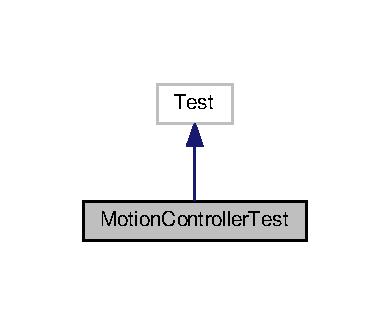
\includegraphics[width=187pt]{classMotionControllerTest__inherit__graph}
\end{center}
\end{figure}


Collaboration diagram for Motion\+Controller\+Test\+:
\nopagebreak
\begin{figure}[H]
\begin{center}
\leavevmode
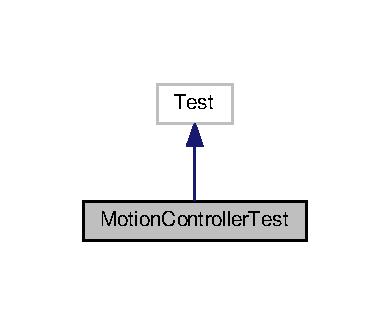
\includegraphics[width=187pt]{classMotionControllerTest__coll__graph}
\end{center}
\end{figure}
\subsection*{Public Member Functions}
\begin{DoxyCompactItemize}
\item 
void \hyperlink{classMotionControllerTest_a6b0cbf29096b0d74ec06488c1be82096}{Set\+Up} ()
\end{DoxyCompactItemize}
\subsection*{Public Attributes}
\begin{DoxyCompactItemize}
\item 
std\+::shared\+\_\+ptr$<$ \hyperlink{classMotionController}{Motion\+Controller} $>$ \hyperlink{classMotionControllerTest_af50a1112a3549fc154026c0078b417ca}{mc}
\end{DoxyCompactItemize}


\subsection{Detailed Description}
\hyperlink{classMotionController}{Motion\+Controller} fixture class. 

\subsection{Member Function Documentation}
\index{Motion\+Controller\+Test@{Motion\+Controller\+Test}!Set\+Up@{Set\+Up}}
\index{Set\+Up@{Set\+Up}!Motion\+Controller\+Test@{Motion\+Controller\+Test}}
\subsubsection[{\texorpdfstring{Set\+Up()}{SetUp()}}]{\setlength{\rightskip}{0pt plus 5cm}void Motion\+Controller\+Test\+::\+Set\+Up (
\begin{DoxyParamCaption}
{}
\end{DoxyParamCaption}
)\hspace{0.3cm}{\ttfamily [inline]}}\hypertarget{classMotionControllerTest_a6b0cbf29096b0d74ec06488c1be82096}{}\label{classMotionControllerTest_a6b0cbf29096b0d74ec06488c1be82096}


\subsection{Member Data Documentation}
\index{Motion\+Controller\+Test@{Motion\+Controller\+Test}!mc@{mc}}
\index{mc@{mc}!Motion\+Controller\+Test@{Motion\+Controller\+Test}}
\subsubsection[{\texorpdfstring{mc}{mc}}]{\setlength{\rightskip}{0pt plus 5cm}std\+::shared\+\_\+ptr$<${\bf Motion\+Controller}$>$ Motion\+Controller\+Test\+::mc}\hypertarget{classMotionControllerTest_af50a1112a3549fc154026c0078b417ca}{}\label{classMotionControllerTest_af50a1112a3549fc154026c0078b417ca}


The documentation for this class was generated from the following file\+:\begin{DoxyCompactItemize}
\item 
/home/ashishpatel/project/src/naivik\+\_\+robot/tests/\hyperlink{motionControllerTest_8cpp}{motion\+Controller\+Test.\+cpp}\end{DoxyCompactItemize}

\hypertarget{classNaivik}{}\section{Naivik Class Reference}
\label{classNaivik}\index{Naivik@{Naivik}}


\hyperlink{classNaivik}{Naivik} class handles the camera and motion controller interactions of the robot.  




{\ttfamily \#include $<$naivik.\+hpp$>$}

\subsection*{Public Member Functions}
\begin{DoxyCompactItemize}
\item 
\hyperlink{classNaivik_a9bc6f959fa714784c3141b08bcbe94c6}{Naivik} (ros\+::\+Node\+Handle nh)
\begin{DoxyCompactList}\small\item\em Overloaded contructor. \end{DoxyCompactList}\item 
\hyperlink{classNaivik_a65ff8b4183c0d11b8ddf041f4be2a933}{$\sim$\+Naivik} ()
\begin{DoxyCompactList}\small\item\em \hyperlink{classNaivik}{Naivik} class destructor. \end{DoxyCompactList}\item 
void \hyperlink{classNaivik_ad4f77bbbbc92e263ac00156d774f7c39}{drive} ()
\begin{DoxyCompactList}\small\item\em Drive the robot using laser scan data. \end{DoxyCompactList}\end{DoxyCompactItemize}
\subsection*{Private Attributes}
\begin{DoxyCompactItemize}
\item 
std\+::shared\+\_\+ptr$<$ \hyperlink{classCamera}{Camera} $>$ \hyperlink{classNaivik_a59456579fab04d7c934dc8826d36821b}{camera\+\_\+} \{nullptr\}
\begin{DoxyCompactList}\small\item\em declare a container for camera class object and initialize it to nullptr \end{DoxyCompactList}\item 
std\+::shared\+\_\+ptr$<$ \hyperlink{classMotionController}{Motion\+Controller} $>$ \hyperlink{classNaivik_a96923f306061a14093c74c5700c1bb8a}{motion\+Controller\+\_\+} \{nullptr\}
\begin{DoxyCompactList}\small\item\em declare a container for \hyperlink{classMotionController}{Motion\+Controller} class object and initialize it to nullptr \end{DoxyCompactList}\item 
ros\+::\+Node\+Handle \hyperlink{classNaivik_af964150f253e4cbaa15bcd1537511af9}{nh\+\_\+}
\begin{DoxyCompactList}\small\item\em declare a container to Node handler for subscribing to services and topics \end{DoxyCompactList}\item 
ros\+::\+Publisher \hyperlink{classNaivik_aaaea1b99cc7f9c6d317e57516564aac9}{velocity\+Publisher\+\_\+}
\begin{DoxyCompactList}\small\item\em declare a container for a R\+OS publisher to publish vehicle motion commands \end{DoxyCompactList}\item 
ros\+::\+Subscriber \hyperlink{classNaivik_a0f001e2ba2dcd1ca7c2fa92eff2c1562}{laser\+Subscriber\+\_\+}
\begin{DoxyCompactList}\small\item\em declare a container for a R\+OS subscriber for laser scan topics \end{DoxyCompactList}\item 
ros\+::\+Subscriber \hyperlink{classNaivik_ab37285b13d04a193f38b2d05a3303694}{camera\+Subscriber\+\_\+}
\begin{DoxyCompactList}\small\item\em declare a container for a R\+OS subscriber for camera topics \end{DoxyCompactList}\item 
ros\+::\+Service\+Server \hyperlink{classNaivik_a7792b0bfe36fe70c679971470b4cc649}{change\+Threshold\+Server\+\_\+}
\begin{DoxyCompactList}\small\item\em declare a container for R\+OS change\+Threshold\+Service \end{DoxyCompactList}\item 
ros\+::\+Service\+Server \hyperlink{classNaivik_a350e4f31ff9ef9e62b2d4b6c9df6fb23}{change\+Linear\+Speed\+Server\+\_\+}
\begin{DoxyCompactList}\small\item\em declare a container for R\+OS change\+Linear\+Speed\+Service \end{DoxyCompactList}\item 
ros\+::\+Service\+Server \hyperlink{classNaivik_a6ead6207d0ce5ef49caa1ad8d1d1fcaa}{change\+Angular\+Speed\+Server\+\_\+}
\begin{DoxyCompactList}\small\item\em declare a container for R\+OS change\+Angular\+Speed\+Service \end{DoxyCompactList}\item 
ros\+::\+Service\+Server \hyperlink{classNaivik_a89a480a5925204ab179dfe0717e26436}{control\+Motion\+Server\+\_\+}
\begin{DoxyCompactList}\small\item\em declare a container for R\+OS control\+Motion\+Service \end{DoxyCompactList}\item 
ros\+::\+Service\+Server \hyperlink{classNaivik_a158e6056518bf811c8aab30f2341e0c6}{take\+Image\+Server\+\_\+}
\begin{DoxyCompactList}\small\item\em declare a container for R\+OS take\+Image\+Service \end{DoxyCompactList}\end{DoxyCompactItemize}


\subsection{Detailed Description}
\hyperlink{classNaivik}{Naivik} class handles the camera and motion controller interactions of the robot. 

\subsection{Constructor \& Destructor Documentation}
\index{Naivik@{Naivik}!Naivik@{Naivik}}
\index{Naivik@{Naivik}!Naivik@{Naivik}}
\subsubsection[{\texorpdfstring{Naivik(ros\+::\+Node\+Handle nh)}{Naivik(ros::NodeHandle nh)}}]{\setlength{\rightskip}{0pt plus 5cm}Naivik\+::\+Naivik (
\begin{DoxyParamCaption}
\item[{ros\+::\+Node\+Handle}]{nh}
\end{DoxyParamCaption}
)\hspace{0.3cm}{\ttfamily [explicit]}}\hypertarget{classNaivik_a9bc6f959fa714784c3141b08bcbe94c6}{}\label{classNaivik_a9bc6f959fa714784c3141b08bcbe94c6}


Overloaded contructor. 


\begin{DoxyParams}{Parameters}
{\em nh} & R\+OS node handle \\
\hline
\end{DoxyParams}
\begin{DoxyReturn}{Returns}
none 
\end{DoxyReturn}
\index{Naivik@{Naivik}!````~Naivik@{$\sim$\+Naivik}}
\index{````~Naivik@{$\sim$\+Naivik}!Naivik@{Naivik}}
\subsubsection[{\texorpdfstring{$\sim$\+Naivik()}{~Naivik()}}]{\setlength{\rightskip}{0pt plus 5cm}Naivik\+::$\sim$\+Naivik (
\begin{DoxyParamCaption}
{}
\end{DoxyParamCaption}
)}\hypertarget{classNaivik_a65ff8b4183c0d11b8ddf041f4be2a933}{}\label{classNaivik_a65ff8b4183c0d11b8ddf041f4be2a933}


\hyperlink{classNaivik}{Naivik} class destructor. 


\begin{DoxyParams}{Parameters}
{\em none} & \\
\hline
\end{DoxyParams}
\begin{DoxyReturn}{Returns}
none 
\end{DoxyReturn}


\subsection{Member Function Documentation}
\index{Naivik@{Naivik}!drive@{drive}}
\index{drive@{drive}!Naivik@{Naivik}}
\subsubsection[{\texorpdfstring{drive()}{drive()}}]{\setlength{\rightskip}{0pt plus 5cm}void Naivik\+::drive (
\begin{DoxyParamCaption}
{}
\end{DoxyParamCaption}
)}\hypertarget{classNaivik_ad4f77bbbbc92e263ac00156d774f7c39}{}\label{classNaivik_ad4f77bbbbc92e263ac00156d774f7c39}


Drive the robot using laser scan data. 


\begin{DoxyParams}{Parameters}
{\em none} & \\
\hline
\end{DoxyParams}
\begin{DoxyReturn}{Returns}
none 
\end{DoxyReturn}


\subsection{Member Data Documentation}
\index{Naivik@{Naivik}!camera\+\_\+@{camera\+\_\+}}
\index{camera\+\_\+@{camera\+\_\+}!Naivik@{Naivik}}
\subsubsection[{\texorpdfstring{camera\+\_\+}{camera_}}]{\setlength{\rightskip}{0pt plus 5cm}std\+::shared\+\_\+ptr$<${\bf Camera}$>$ Naivik\+::camera\+\_\+ \{nullptr\}\hspace{0.3cm}{\ttfamily [private]}}\hypertarget{classNaivik_a59456579fab04d7c934dc8826d36821b}{}\label{classNaivik_a59456579fab04d7c934dc8826d36821b}


declare a container for camera class object and initialize it to nullptr 

\index{Naivik@{Naivik}!camera\+Subscriber\+\_\+@{camera\+Subscriber\+\_\+}}
\index{camera\+Subscriber\+\_\+@{camera\+Subscriber\+\_\+}!Naivik@{Naivik}}
\subsubsection[{\texorpdfstring{camera\+Subscriber\+\_\+}{cameraSubscriber_}}]{\setlength{\rightskip}{0pt plus 5cm}ros\+::\+Subscriber Naivik\+::camera\+Subscriber\+\_\+\hspace{0.3cm}{\ttfamily [private]}}\hypertarget{classNaivik_ab37285b13d04a193f38b2d05a3303694}{}\label{classNaivik_ab37285b13d04a193f38b2d05a3303694}


declare a container for a R\+OS subscriber for camera topics 

\index{Naivik@{Naivik}!change\+Angular\+Speed\+Server\+\_\+@{change\+Angular\+Speed\+Server\+\_\+}}
\index{change\+Angular\+Speed\+Server\+\_\+@{change\+Angular\+Speed\+Server\+\_\+}!Naivik@{Naivik}}
\subsubsection[{\texorpdfstring{change\+Angular\+Speed\+Server\+\_\+}{changeAngularSpeedServer_}}]{\setlength{\rightskip}{0pt plus 5cm}ros\+::\+Service\+Server Naivik\+::change\+Angular\+Speed\+Server\+\_\+\hspace{0.3cm}{\ttfamily [private]}}\hypertarget{classNaivik_a6ead6207d0ce5ef49caa1ad8d1d1fcaa}{}\label{classNaivik_a6ead6207d0ce5ef49caa1ad8d1d1fcaa}


declare a container for R\+OS change\+Angular\+Speed\+Service 

\index{Naivik@{Naivik}!change\+Linear\+Speed\+Server\+\_\+@{change\+Linear\+Speed\+Server\+\_\+}}
\index{change\+Linear\+Speed\+Server\+\_\+@{change\+Linear\+Speed\+Server\+\_\+}!Naivik@{Naivik}}
\subsubsection[{\texorpdfstring{change\+Linear\+Speed\+Server\+\_\+}{changeLinearSpeedServer_}}]{\setlength{\rightskip}{0pt plus 5cm}ros\+::\+Service\+Server Naivik\+::change\+Linear\+Speed\+Server\+\_\+\hspace{0.3cm}{\ttfamily [private]}}\hypertarget{classNaivik_a350e4f31ff9ef9e62b2d4b6c9df6fb23}{}\label{classNaivik_a350e4f31ff9ef9e62b2d4b6c9df6fb23}


declare a container for R\+OS change\+Linear\+Speed\+Service 

\index{Naivik@{Naivik}!change\+Threshold\+Server\+\_\+@{change\+Threshold\+Server\+\_\+}}
\index{change\+Threshold\+Server\+\_\+@{change\+Threshold\+Server\+\_\+}!Naivik@{Naivik}}
\subsubsection[{\texorpdfstring{change\+Threshold\+Server\+\_\+}{changeThresholdServer_}}]{\setlength{\rightskip}{0pt plus 5cm}ros\+::\+Service\+Server Naivik\+::change\+Threshold\+Server\+\_\+\hspace{0.3cm}{\ttfamily [private]}}\hypertarget{classNaivik_a7792b0bfe36fe70c679971470b4cc649}{}\label{classNaivik_a7792b0bfe36fe70c679971470b4cc649}


declare a container for R\+OS change\+Threshold\+Service 

\index{Naivik@{Naivik}!control\+Motion\+Server\+\_\+@{control\+Motion\+Server\+\_\+}}
\index{control\+Motion\+Server\+\_\+@{control\+Motion\+Server\+\_\+}!Naivik@{Naivik}}
\subsubsection[{\texorpdfstring{control\+Motion\+Server\+\_\+}{controlMotionServer_}}]{\setlength{\rightskip}{0pt plus 5cm}ros\+::\+Service\+Server Naivik\+::control\+Motion\+Server\+\_\+\hspace{0.3cm}{\ttfamily [private]}}\hypertarget{classNaivik_a89a480a5925204ab179dfe0717e26436}{}\label{classNaivik_a89a480a5925204ab179dfe0717e26436}


declare a container for R\+OS control\+Motion\+Service 

\index{Naivik@{Naivik}!laser\+Subscriber\+\_\+@{laser\+Subscriber\+\_\+}}
\index{laser\+Subscriber\+\_\+@{laser\+Subscriber\+\_\+}!Naivik@{Naivik}}
\subsubsection[{\texorpdfstring{laser\+Subscriber\+\_\+}{laserSubscriber_}}]{\setlength{\rightskip}{0pt plus 5cm}ros\+::\+Subscriber Naivik\+::laser\+Subscriber\+\_\+\hspace{0.3cm}{\ttfamily [private]}}\hypertarget{classNaivik_a0f001e2ba2dcd1ca7c2fa92eff2c1562}{}\label{classNaivik_a0f001e2ba2dcd1ca7c2fa92eff2c1562}


declare a container for a R\+OS subscriber for laser scan topics 

\index{Naivik@{Naivik}!motion\+Controller\+\_\+@{motion\+Controller\+\_\+}}
\index{motion\+Controller\+\_\+@{motion\+Controller\+\_\+}!Naivik@{Naivik}}
\subsubsection[{\texorpdfstring{motion\+Controller\+\_\+}{motionController_}}]{\setlength{\rightskip}{0pt plus 5cm}std\+::shared\+\_\+ptr$<${\bf Motion\+Controller}$>$ Naivik\+::motion\+Controller\+\_\+ \{nullptr\}\hspace{0.3cm}{\ttfamily [private]}}\hypertarget{classNaivik_a96923f306061a14093c74c5700c1bb8a}{}\label{classNaivik_a96923f306061a14093c74c5700c1bb8a}


declare a container for \hyperlink{classMotionController}{Motion\+Controller} class object and initialize it to nullptr 

\index{Naivik@{Naivik}!nh\+\_\+@{nh\+\_\+}}
\index{nh\+\_\+@{nh\+\_\+}!Naivik@{Naivik}}
\subsubsection[{\texorpdfstring{nh\+\_\+}{nh_}}]{\setlength{\rightskip}{0pt plus 5cm}ros\+::\+Node\+Handle Naivik\+::nh\+\_\+\hspace{0.3cm}{\ttfamily [private]}}\hypertarget{classNaivik_af964150f253e4cbaa15bcd1537511af9}{}\label{classNaivik_af964150f253e4cbaa15bcd1537511af9}


declare a container to Node handler for subscribing to services and topics 

\index{Naivik@{Naivik}!take\+Image\+Server\+\_\+@{take\+Image\+Server\+\_\+}}
\index{take\+Image\+Server\+\_\+@{take\+Image\+Server\+\_\+}!Naivik@{Naivik}}
\subsubsection[{\texorpdfstring{take\+Image\+Server\+\_\+}{takeImageServer_}}]{\setlength{\rightskip}{0pt plus 5cm}ros\+::\+Service\+Server Naivik\+::take\+Image\+Server\+\_\+\hspace{0.3cm}{\ttfamily [private]}}\hypertarget{classNaivik_a158e6056518bf811c8aab30f2341e0c6}{}\label{classNaivik_a158e6056518bf811c8aab30f2341e0c6}


declare a container for R\+OS take\+Image\+Service 

\index{Naivik@{Naivik}!velocity\+Publisher\+\_\+@{velocity\+Publisher\+\_\+}}
\index{velocity\+Publisher\+\_\+@{velocity\+Publisher\+\_\+}!Naivik@{Naivik}}
\subsubsection[{\texorpdfstring{velocity\+Publisher\+\_\+}{velocityPublisher_}}]{\setlength{\rightskip}{0pt plus 5cm}ros\+::\+Publisher Naivik\+::velocity\+Publisher\+\_\+\hspace{0.3cm}{\ttfamily [private]}}\hypertarget{classNaivik_aaaea1b99cc7f9c6d317e57516564aac9}{}\label{classNaivik_aaaea1b99cc7f9c6d317e57516564aac9}


declare a container for a R\+OS publisher to publish vehicle motion commands 



The documentation for this class was generated from the following files\+:\begin{DoxyCompactItemize}
\item 
/home/ashishpatel/project/src/naivik\+\_\+robot/include/\hyperlink{naivik_8hpp}{naivik.\+hpp}\item 
/home/ashishpatel/project/src/naivik\+\_\+robot/src/\hyperlink{naivik_8cpp}{naivik.\+cpp}\end{DoxyCompactItemize}

\hypertarget{classNaivikTest}{}\section{Naivik\+Test Class Reference}
\label{classNaivikTest}\index{Naivik\+Test@{Naivik\+Test}}


\hyperlink{classNaivik}{Naivik} fixture class.  




Inheritance diagram for Naivik\+Test\+:
\nopagebreak
\begin{figure}[H]
\begin{center}
\leavevmode
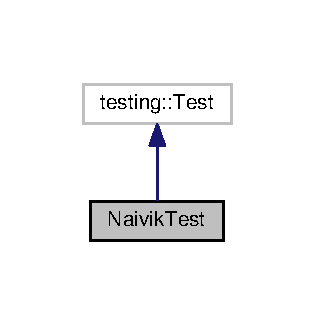
\includegraphics[width=151pt]{classNaivikTest__inherit__graph}
\end{center}
\end{figure}


Collaboration diagram for Naivik\+Test\+:
\nopagebreak
\begin{figure}[H]
\begin{center}
\leavevmode
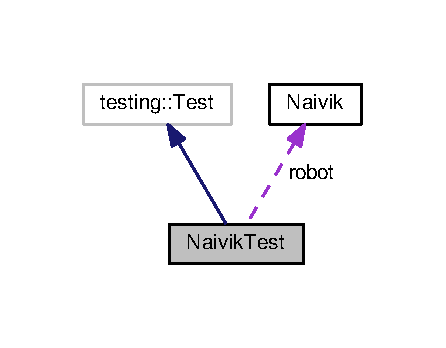
\includegraphics[width=214pt]{classNaivikTest__coll__graph}
\end{center}
\end{figure}
\subsection*{Public Member Functions}
\begin{DoxyCompactItemize}
\item 
void \hyperlink{classNaivikTest_a86ab33fa14f17c2dab8ddd683e566107}{Set\+Up} ()
\end{DoxyCompactItemize}
\subsection*{Public Attributes}
\begin{DoxyCompactItemize}
\item 
\hyperlink{classNaivik}{Naivik} \hyperlink{classNaivikTest_ad27ff26b26e11e6c7cbb7e71f6e7b608}{robot}
\end{DoxyCompactItemize}


\subsection{Detailed Description}
\hyperlink{classNaivik}{Naivik} fixture class. 

\subsection{Member Function Documentation}
\index{Naivik\+Test@{Naivik\+Test}!Set\+Up@{Set\+Up}}
\index{Set\+Up@{Set\+Up}!Naivik\+Test@{Naivik\+Test}}
\subsubsection[{\texorpdfstring{Set\+Up()}{SetUp()}}]{\setlength{\rightskip}{0pt plus 5cm}void Naivik\+Test\+::\+Set\+Up (
\begin{DoxyParamCaption}
{}
\end{DoxyParamCaption}
)\hspace{0.3cm}{\ttfamily [inline]}}\hypertarget{classNaivikTest_a86ab33fa14f17c2dab8ddd683e566107}{}\label{classNaivikTest_a86ab33fa14f17c2dab8ddd683e566107}


\subsection{Member Data Documentation}
\index{Naivik\+Test@{Naivik\+Test}!robot@{robot}}
\index{robot@{robot}!Naivik\+Test@{Naivik\+Test}}
\subsubsection[{\texorpdfstring{robot}{robot}}]{\setlength{\rightskip}{0pt plus 5cm}{\bf Naivik} Naivik\+Test\+::robot}\hypertarget{classNaivikTest_ad27ff26b26e11e6c7cbb7e71f6e7b608}{}\label{classNaivikTest_ad27ff26b26e11e6c7cbb7e71f6e7b608}


The documentation for this class was generated from the following file\+:\begin{DoxyCompactItemize}
\item 
/home/ashishpatel/project/src/naivik\+\_\+robot/tests/\hyperlink{naivikTest_8cpp}{naivik\+Test.\+cpp}\end{DoxyCompactItemize}

\hypertarget{classObstacleDetection}{}\section{Obstacle\+Detection Class Reference}
\label{classObstacleDetection}\index{Obstacle\+Detection@{Obstacle\+Detection}}


\hyperlink{classObstacleDetection}{Obstacle\+Detection} class handles determining if the vehicle is going to collide using laser scans data.  




{\ttfamily \#include $<$obstacle\+Detection.\+hpp$>$}

\subsection*{Public Member Functions}
\begin{DoxyCompactItemize}
\item 
\hyperlink{classObstacleDetection_afb1806d3b8806f9d269bc29b8e8c6ac9}{Obstacle\+Detection} (double dist\+Threshold)
\begin{DoxyCompactList}\small\item\em \hyperlink{classObstacleDetection}{Obstacle\+Detection} class overloaded constructor. \end{DoxyCompactList}\item 
\hyperlink{classObstacleDetection_a72cb5fb0b56c1c3b6e4ab42da46e28e9}{$\sim$\+Obstacle\+Detection} ()
\begin{DoxyCompactList}\small\item\em \hyperlink{classObstacleDetection}{Obstacle\+Detection} class destructor. \end{DoxyCompactList}\item 
bool \hyperlink{classObstacleDetection_a99de70aa28dfaa9f1c2770e3d744a4cc}{detect\+Obstacle} (const sensor\+\_\+msgs\+::\+Laser\+Scan\+::\+Const\+Ptr \&msg)
\begin{DoxyCompactList}\small\item\em Detects the Obstacle in front of the robot. \end{DoxyCompactList}\item 
void \hyperlink{classObstacleDetection_a7168393889737f1798acafa452a6a69a}{set\+Dist\+Threshold} (double threshold)
\begin{DoxyCompactList}\small\item\em set dist\+Threshold value \end{DoxyCompactList}\item 
double \hyperlink{classObstacleDetection_aae290781954d75c8e90517e6ac39c7d1}{get\+Dist\+Threshold} ()
\begin{DoxyCompactList}\small\item\em get dist\+Threshold value \end{DoxyCompactList}\end{DoxyCompactItemize}
\subsection*{Private Attributes}
\begin{DoxyCompactItemize}
\item 
double \hyperlink{classObstacleDetection_a594c4476745d0404a07135465f9e04e7}{dist\+Threshold\+\_\+} \{0.\+0\}
\begin{DoxyCompactList}\small\item\em declare a container to determine how close the robot should get to an object \end{DoxyCompactList}\end{DoxyCompactItemize}


\subsection{Detailed Description}
\hyperlink{classObstacleDetection}{Obstacle\+Detection} class handles determining if the vehicle is going to collide using laser scans data. 

\subsection{Constructor \& Destructor Documentation}
\index{Obstacle\+Detection@{Obstacle\+Detection}!Obstacle\+Detection@{Obstacle\+Detection}}
\index{Obstacle\+Detection@{Obstacle\+Detection}!Obstacle\+Detection@{Obstacle\+Detection}}
\subsubsection[{\texorpdfstring{Obstacle\+Detection(double dist\+Threshold)}{ObstacleDetection(double distThreshold)}}]{\setlength{\rightskip}{0pt plus 5cm}Obstacle\+Detection\+::\+Obstacle\+Detection (
\begin{DoxyParamCaption}
\item[{double}]{dist\+Threshold}
\end{DoxyParamCaption}
)\hspace{0.3cm}{\ttfamily [explicit]}}\hypertarget{classObstacleDetection_afb1806d3b8806f9d269bc29b8e8c6ac9}{}\label{classObstacleDetection_afb1806d3b8806f9d269bc29b8e8c6ac9}


\hyperlink{classObstacleDetection}{Obstacle\+Detection} class overloaded constructor. 


\begin{DoxyParams}{Parameters}
{\em dist\+Threshold} & of type double \\
\hline
\end{DoxyParams}
\begin{DoxyReturn}{Returns}
none 
\end{DoxyReturn}
\index{Obstacle\+Detection@{Obstacle\+Detection}!````~Obstacle\+Detection@{$\sim$\+Obstacle\+Detection}}
\index{````~Obstacle\+Detection@{$\sim$\+Obstacle\+Detection}!Obstacle\+Detection@{Obstacle\+Detection}}
\subsubsection[{\texorpdfstring{$\sim$\+Obstacle\+Detection()}{~ObstacleDetection()}}]{\setlength{\rightskip}{0pt plus 5cm}Obstacle\+Detection\+::$\sim$\+Obstacle\+Detection (
\begin{DoxyParamCaption}
{}
\end{DoxyParamCaption}
)}\hypertarget{classObstacleDetection_a72cb5fb0b56c1c3b6e4ab42da46e28e9}{}\label{classObstacleDetection_a72cb5fb0b56c1c3b6e4ab42da46e28e9}


\hyperlink{classObstacleDetection}{Obstacle\+Detection} class destructor. 


\begin{DoxyParams}{Parameters}
{\em none} & \\
\hline
\end{DoxyParams}
\begin{DoxyReturn}{Returns}
none 
\end{DoxyReturn}


\subsection{Member Function Documentation}
\index{Obstacle\+Detection@{Obstacle\+Detection}!detect\+Obstacle@{detect\+Obstacle}}
\index{detect\+Obstacle@{detect\+Obstacle}!Obstacle\+Detection@{Obstacle\+Detection}}
\subsubsection[{\texorpdfstring{detect\+Obstacle(const sensor\+\_\+msgs\+::\+Laser\+Scan\+::\+Const\+Ptr \&msg)}{detectObstacle(const sensor_msgs::LaserScan::ConstPtr &msg)}}]{\setlength{\rightskip}{0pt plus 5cm}bool Obstacle\+Detection\+::detect\+Obstacle (
\begin{DoxyParamCaption}
\item[{const sensor\+\_\+msgs\+::\+Laser\+Scan\+::\+Const\+Ptr \&}]{msg}
\end{DoxyParamCaption}
)}\hypertarget{classObstacleDetection_a99de70aa28dfaa9f1c2770e3d744a4cc}{}\label{classObstacleDetection_a99de70aa28dfaa9f1c2770e3d744a4cc}


Detects the Obstacle in front of the robot. 


\begin{DoxyParams}{Parameters}
{\em a} & reference to a variable of type sensor\+\_\+msgs\+::\+Laser\+Scan \\
\hline
\end{DoxyParams}
\begin{DoxyReturn}{Returns}
true, if obstacle is detected false, if obstacle is not detected 
\end{DoxyReturn}
\index{Obstacle\+Detection@{Obstacle\+Detection}!get\+Dist\+Threshold@{get\+Dist\+Threshold}}
\index{get\+Dist\+Threshold@{get\+Dist\+Threshold}!Obstacle\+Detection@{Obstacle\+Detection}}
\subsubsection[{\texorpdfstring{get\+Dist\+Threshold()}{getDistThreshold()}}]{\setlength{\rightskip}{0pt plus 5cm}double Obstacle\+Detection\+::get\+Dist\+Threshold (
\begin{DoxyParamCaption}
{}
\end{DoxyParamCaption}
)}\hypertarget{classObstacleDetection_aae290781954d75c8e90517e6ac39c7d1}{}\label{classObstacleDetection_aae290781954d75c8e90517e6ac39c7d1}


get dist\+Threshold value 


\begin{DoxyParams}{Parameters}
{\em none} & \\
\hline
\end{DoxyParams}
\begin{DoxyReturn}{Returns}
dist\+Threshold of type double 
\end{DoxyReturn}
\index{Obstacle\+Detection@{Obstacle\+Detection}!set\+Dist\+Threshold@{set\+Dist\+Threshold}}
\index{set\+Dist\+Threshold@{set\+Dist\+Threshold}!Obstacle\+Detection@{Obstacle\+Detection}}
\subsubsection[{\texorpdfstring{set\+Dist\+Threshold(double threshold)}{setDistThreshold(double threshold)}}]{\setlength{\rightskip}{0pt plus 5cm}void Obstacle\+Detection\+::set\+Dist\+Threshold (
\begin{DoxyParamCaption}
\item[{double}]{threshold}
\end{DoxyParamCaption}
)}\hypertarget{classObstacleDetection_a7168393889737f1798acafa452a6a69a}{}\label{classObstacleDetection_a7168393889737f1798acafa452a6a69a}


set dist\+Threshold value 


\begin{DoxyParams}{Parameters}
{\em threshold} & of type double \\
\hline
\end{DoxyParams}
\begin{DoxyReturn}{Returns}
none 
\end{DoxyReturn}


\subsection{Member Data Documentation}
\index{Obstacle\+Detection@{Obstacle\+Detection}!dist\+Threshold\+\_\+@{dist\+Threshold\+\_\+}}
\index{dist\+Threshold\+\_\+@{dist\+Threshold\+\_\+}!Obstacle\+Detection@{Obstacle\+Detection}}
\subsubsection[{\texorpdfstring{dist\+Threshold\+\_\+}{distThreshold_}}]{\setlength{\rightskip}{0pt plus 5cm}double Obstacle\+Detection\+::dist\+Threshold\+\_\+ \{0.\+0\}\hspace{0.3cm}{\ttfamily [private]}}\hypertarget{classObstacleDetection_a594c4476745d0404a07135465f9e04e7}{}\label{classObstacleDetection_a594c4476745d0404a07135465f9e04e7}


declare a container to determine how close the robot should get to an object 



The documentation for this class was generated from the following files\+:\begin{DoxyCompactItemize}
\item 
/home/ashishpatel/project/src/naivik\+\_\+robot/include/\hyperlink{obstacleDetection_8hpp}{obstacle\+Detection.\+hpp}\item 
/home/ashishpatel/project/src/naivik\+\_\+robot/src/\hyperlink{obstacleDetection_8cpp}{obstacle\+Detection.\+cpp}\end{DoxyCompactItemize}

\hypertarget{classObstacleDetectionTest}{}\section{Obstacle\+Detection\+Test Class Reference}
\label{classObstacleDetectionTest}\index{Obstacle\+Detection\+Test@{Obstacle\+Detection\+Test}}


\hyperlink{classObstacleDetection}{Obstacle\+Detection} fixture class.  




Inheritance diagram for Obstacle\+Detection\+Test\+:
\nopagebreak
\begin{figure}[H]
\begin{center}
\leavevmode
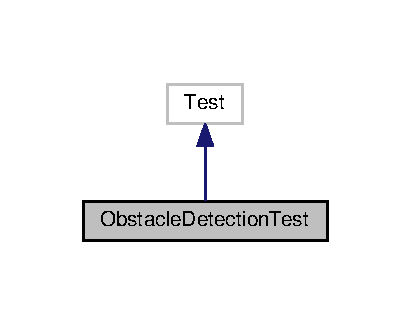
\includegraphics[width=197pt]{classObstacleDetectionTest__inherit__graph}
\end{center}
\end{figure}


Collaboration diagram for Obstacle\+Detection\+Test\+:
\nopagebreak
\begin{figure}[H]
\begin{center}
\leavevmode
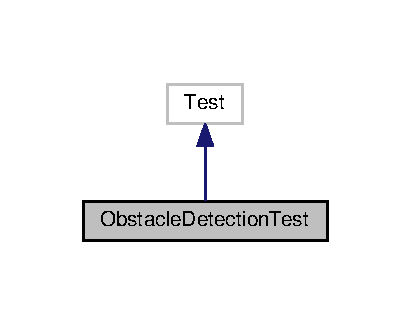
\includegraphics[width=197pt]{classObstacleDetectionTest__coll__graph}
\end{center}
\end{figure}
\subsection*{Public Member Functions}
\begin{DoxyCompactItemize}
\item 
void \hyperlink{classObstacleDetectionTest_af8f279787b436f2ee1c84de7eab1df27}{Set\+Up} ()
\end{DoxyCompactItemize}
\subsection*{Public Attributes}
\begin{DoxyCompactItemize}
\item 
std\+::shared\+\_\+ptr$<$ \hyperlink{classObstacleDetection}{Obstacle\+Detection} $>$ \hyperlink{classObstacleDetectionTest_a42128dc8d1443e3fa9c52a60a8009b03}{obs}
\end{DoxyCompactItemize}


\subsection{Detailed Description}
\hyperlink{classObstacleDetection}{Obstacle\+Detection} fixture class. 

\subsection{Member Function Documentation}
\index{Obstacle\+Detection\+Test@{Obstacle\+Detection\+Test}!Set\+Up@{Set\+Up}}
\index{Set\+Up@{Set\+Up}!Obstacle\+Detection\+Test@{Obstacle\+Detection\+Test}}
\subsubsection[{\texorpdfstring{Set\+Up()}{SetUp()}}]{\setlength{\rightskip}{0pt plus 5cm}void Obstacle\+Detection\+Test\+::\+Set\+Up (
\begin{DoxyParamCaption}
{}
\end{DoxyParamCaption}
)\hspace{0.3cm}{\ttfamily [inline]}}\hypertarget{classObstacleDetectionTest_af8f279787b436f2ee1c84de7eab1df27}{}\label{classObstacleDetectionTest_af8f279787b436f2ee1c84de7eab1df27}


\subsection{Member Data Documentation}
\index{Obstacle\+Detection\+Test@{Obstacle\+Detection\+Test}!obs@{obs}}
\index{obs@{obs}!Obstacle\+Detection\+Test@{Obstacle\+Detection\+Test}}
\subsubsection[{\texorpdfstring{obs}{obs}}]{\setlength{\rightskip}{0pt plus 5cm}std\+::shared\+\_\+ptr$<${\bf Obstacle\+Detection}$>$ Obstacle\+Detection\+Test\+::obs}\hypertarget{classObstacleDetectionTest_a42128dc8d1443e3fa9c52a60a8009b03}{}\label{classObstacleDetectionTest_a42128dc8d1443e3fa9c52a60a8009b03}


The documentation for this class was generated from the following file\+:\begin{DoxyCompactItemize}
\item 
/home/ashishpatel/project/src/naivik\+\_\+robot/tests/\hyperlink{obstacleDetectionTest_8cpp}{obstacle\+Detection\+Test.\+cpp}\end{DoxyCompactItemize}

\hypertarget{classTestHelper}{}\section{Test\+Helper Class Reference}
\label{classTestHelper}\index{Test\+Helper@{Test\+Helper}}


\hyperlink{classTestHelper}{Test\+Helper} class handles in testing the nodes publisher and subscriber.  




{\ttfamily \#include $<$test\+Helper.\+hpp$>$}

\subsection*{Public Member Functions}
\begin{DoxyCompactItemize}
\item 
\hyperlink{classTestHelper_ae17c73ef2a5c492a3602ac49a0b11c96}{Test\+Helper} ()
\begin{DoxyCompactList}\small\item\em \hyperlink{classTestHelper}{Test\+Helper} class constructor. \end{DoxyCompactList}\item 
\hyperlink{classTestHelper_a6924609e765a4b5bba0cf322ae0568ec}{$\sim$\+Test\+Helper} ()
\begin{DoxyCompactList}\small\item\em \hyperlink{classTestHelper}{Test\+Helper} class destructor. \end{DoxyCompactList}\item 
void \hyperlink{classTestHelper_adb16c8e17de51d68a53f2ff9ead44589}{velocity\+Callback} (const geometry\+\_\+msgs\+::\+Twist\+::\+Const\+Ptr \&msg)
\begin{DoxyCompactList}\small\item\em Callback function for velocity messages. \end{DoxyCompactList}\end{DoxyCompactItemize}
\subsection*{Public Attributes}
\begin{DoxyCompactItemize}
\item 
geometry\+\_\+msgs\+::\+Twist \hyperlink{classTestHelper_a78a826fd3e1a4bc10adc910cde81668d}{twist}
\begin{DoxyCompactList}\small\item\em declare a container for storing robot velocity messages \end{DoxyCompactList}\end{DoxyCompactItemize}


\subsection{Detailed Description}
\hyperlink{classTestHelper}{Test\+Helper} class handles in testing the nodes publisher and subscriber. 

\subsection{Constructor \& Destructor Documentation}
\index{Test\+Helper@{Test\+Helper}!Test\+Helper@{Test\+Helper}}
\index{Test\+Helper@{Test\+Helper}!Test\+Helper@{Test\+Helper}}
\subsubsection[{\texorpdfstring{Test\+Helper()}{TestHelper()}}]{\setlength{\rightskip}{0pt plus 5cm}Test\+Helper\+::\+Test\+Helper (
\begin{DoxyParamCaption}
{}
\end{DoxyParamCaption}
)}\hypertarget{classTestHelper_ae17c73ef2a5c492a3602ac49a0b11c96}{}\label{classTestHelper_ae17c73ef2a5c492a3602ac49a0b11c96}


\hyperlink{classTestHelper}{Test\+Helper} class constructor. 


\begin{DoxyParams}{Parameters}
{\em none} & \\
\hline
\end{DoxyParams}
\begin{DoxyReturn}{Returns}
none 
\end{DoxyReturn}
\index{Test\+Helper@{Test\+Helper}!````~Test\+Helper@{$\sim$\+Test\+Helper}}
\index{````~Test\+Helper@{$\sim$\+Test\+Helper}!Test\+Helper@{Test\+Helper}}
\subsubsection[{\texorpdfstring{$\sim$\+Test\+Helper()}{~TestHelper()}}]{\setlength{\rightskip}{0pt plus 5cm}Test\+Helper\+::$\sim$\+Test\+Helper (
\begin{DoxyParamCaption}
{}
\end{DoxyParamCaption}
)}\hypertarget{classTestHelper_a6924609e765a4b5bba0cf322ae0568ec}{}\label{classTestHelper_a6924609e765a4b5bba0cf322ae0568ec}


\hyperlink{classTestHelper}{Test\+Helper} class destructor. 


\begin{DoxyParams}{Parameters}
{\em none} & \\
\hline
\end{DoxyParams}
\begin{DoxyReturn}{Returns}
none 
\end{DoxyReturn}


\subsection{Member Function Documentation}
\index{Test\+Helper@{Test\+Helper}!velocity\+Callback@{velocity\+Callback}}
\index{velocity\+Callback@{velocity\+Callback}!Test\+Helper@{Test\+Helper}}
\subsubsection[{\texorpdfstring{velocity\+Callback(const geometry\+\_\+msgs\+::\+Twist\+::\+Const\+Ptr \&msg)}{velocityCallback(const geometry_msgs::Twist::ConstPtr &msg)}}]{\setlength{\rightskip}{0pt plus 5cm}void Test\+Helper\+::velocity\+Callback (
\begin{DoxyParamCaption}
\item[{const geometry\+\_\+msgs\+::\+Twist\+::\+Const\+Ptr \&}]{msg}
\end{DoxyParamCaption}
)}\hypertarget{classTestHelper_adb16c8e17de51d68a53f2ff9ead44589}{}\label{classTestHelper_adb16c8e17de51d68a53f2ff9ead44589}


Callback function for velocity messages. 


\begin{DoxyParams}{Parameters}
{\em a} & reference to a variable of type geometry\+\_\+msgs\+::\+Twist \\
\hline
\end{DoxyParams}
\begin{DoxyReturn}{Returns}
none 
\end{DoxyReturn}


\subsection{Member Data Documentation}
\index{Test\+Helper@{Test\+Helper}!twist@{twist}}
\index{twist@{twist}!Test\+Helper@{Test\+Helper}}
\subsubsection[{\texorpdfstring{twist}{twist}}]{\setlength{\rightskip}{0pt plus 5cm}geometry\+\_\+msgs\+::\+Twist Test\+Helper\+::twist}\hypertarget{classTestHelper_a78a826fd3e1a4bc10adc910cde81668d}{}\label{classTestHelper_a78a826fd3e1a4bc10adc910cde81668d}


declare a container for storing robot velocity messages 



The documentation for this class was generated from the following files\+:\begin{DoxyCompactItemize}
\item 
/home/ashishpatel/project/src/naivik\+\_\+robot/tests/\hyperlink{testHelper_8hpp}{test\+Helper.\+hpp}\item 
/home/ashishpatel/project/src/naivik\+\_\+robot/tests/\hyperlink{testHelper_8cpp}{test\+Helper.\+cpp}\end{DoxyCompactItemize}

\chapter{File Documentation}
\hypertarget{camera_8hpp}{}\section{/home/ashishpatel/project/src/naivik\+\_\+robot/include/camera.hpp File Reference}
\label{camera_8hpp}\index{/home/ashishpatel/project/src/naivik\+\_\+robot/include/camera.\+hpp@{/home/ashishpatel/project/src/naivik\+\_\+robot/include/camera.\+hpp}}


\hyperlink{classCamera}{Camera} class header file.  


{\ttfamily \#include $<$memory$>$}\\*
{\ttfamily \#include $<$string$>$}\\*
{\ttfamily \#include $<$vector$>$}\\*
{\ttfamily \#include $<$sstream$>$}\\*
{\ttfamily \#include \char`\"{}ros/ros.\+h\char`\"{}}\\*
{\ttfamily \#include \char`\"{}image\+\_\+transport/image\+\_\+transport.\+h\char`\"{}}\\*
{\ttfamily \#include \char`\"{}cv\+\_\+bridge/cv\+\_\+bridge.\+h\char`\"{}}\\*
{\ttfamily \#include \char`\"{}sensor\+\_\+msgs/image\+\_\+encodings.\+h\char`\"{}}\\*
{\ttfamily \#include \char`\"{}sensor\+\_\+msgs/\+Image.\+h\char`\"{}}\\*
{\ttfamily \#include \char`\"{}opencv2/imgproc/imgproc.\+hpp\char`\"{}}\\*
{\ttfamily \#include \char`\"{}opencv2/core/core.\+hpp\char`\"{}}\\*
{\ttfamily \#include \char`\"{}opencv2/highgui/highgui.\+hpp\char`\"{}}\\*
{\ttfamily \#include \char`\"{}naivik\+\_\+robot/take\+Image\+Service.\+h\char`\"{}}\\*
Include dependency graph for camera.\+hpp\+:
\nopagebreak
\begin{figure}[H]
\begin{center}
\leavevmode
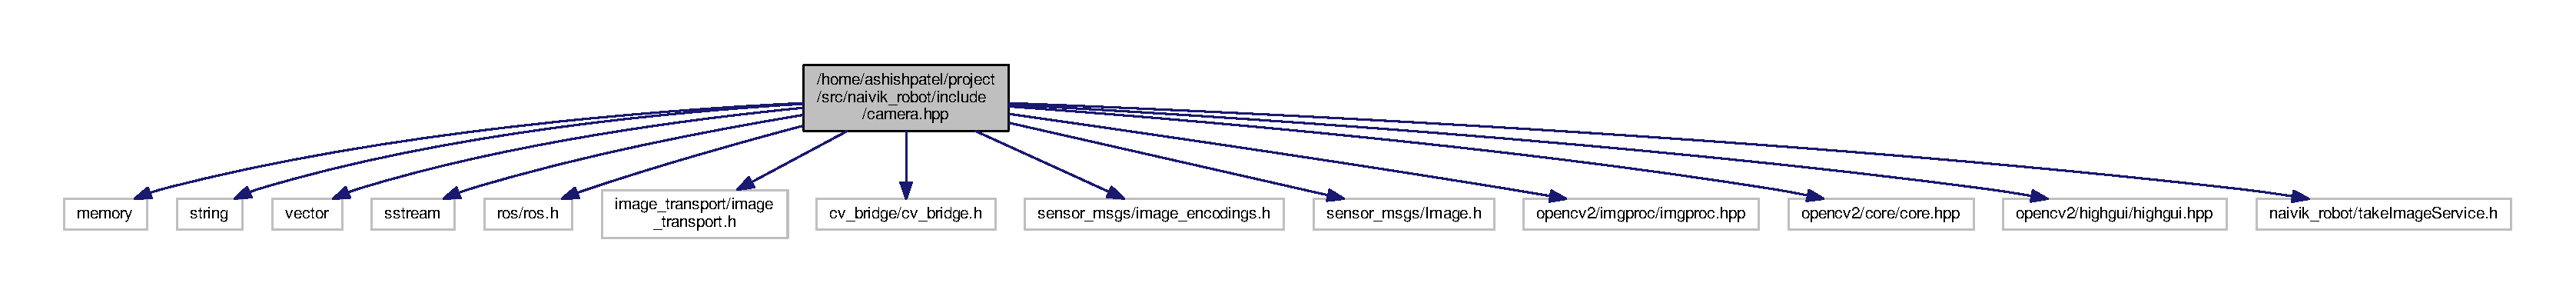
\includegraphics[width=350pt]{camera_8hpp__incl}
\end{center}
\end{figure}
This graph shows which files directly or indirectly include this file\+:
\nopagebreak
\begin{figure}[H]
\begin{center}
\leavevmode
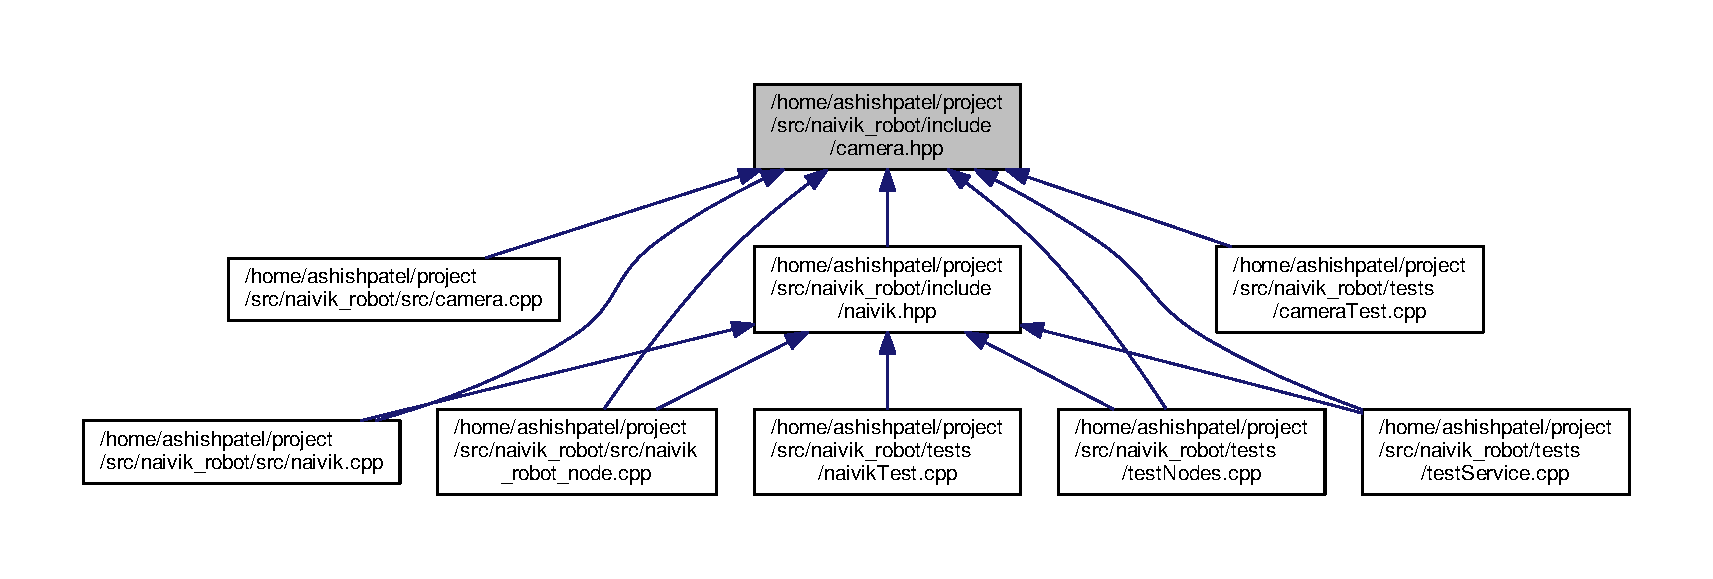
\includegraphics[width=350pt]{camera_8hpp__dep__incl}
\end{center}
\end{figure}
\subsection*{Classes}
\begin{DoxyCompactItemize}
\item 
class \hyperlink{classCamera}{Camera}
\begin{DoxyCompactList}\small\item\em \hyperlink{classCamera}{Camera} class handles viewing and taking images in front of the robot. \end{DoxyCompactList}\end{DoxyCompactItemize}


\subsection{Detailed Description}
\hyperlink{classCamera}{Camera} class header file. 

M\+IT License

Copyright (c) 2018 Ashish Patel

Permission is hereby granted, free of charge, to any person obtaining a copy of this software and associated documentation files (the \char`\"{}\+Software\char`\"{}), to deal in the Software without restriction, including without limitation the rights to use, copy, modify, merge, publish, distribute, sublicense, and/or sell copies of the Software, and to permit persons to whom the Software is furnished to do so, subject to the following conditions\+:

The above copyright notice and this permission notice shall be included in all copies or substantial portions of the Software.

T\+HE S\+O\+F\+T\+W\+A\+RE IS P\+R\+O\+V\+I\+D\+ED \char`\"{}\+A\+S I\+S\char`\"{}, W\+I\+T\+H\+O\+UT W\+A\+R\+R\+A\+N\+TY OF A\+NY K\+I\+ND, E\+X\+P\+R\+E\+SS OR I\+M\+P\+L\+I\+ED, I\+N\+C\+L\+U\+D\+I\+NG B\+UT N\+OT L\+I\+M\+I\+T\+ED TO T\+HE W\+A\+R\+R\+A\+N\+T\+I\+ES OF M\+E\+R\+C\+H\+A\+N\+T\+A\+B\+I\+L\+I\+TY, F\+I\+T\+N\+E\+SS F\+OR A P\+A\+R\+T\+I\+C\+U\+L\+AR P\+U\+R\+P\+O\+SE A\+ND N\+O\+N\+I\+N\+F\+R\+I\+N\+G\+E\+M\+E\+NT. IN NO E\+V\+E\+NT S\+H\+A\+LL T\+HE A\+U\+T\+H\+O\+RS OR C\+O\+P\+Y\+R\+I\+G\+HT H\+O\+L\+D\+E\+RS BE L\+I\+A\+B\+LE F\+OR A\+NY C\+L\+A\+IM, D\+A\+M\+A\+G\+ES OR O\+T\+H\+ER L\+I\+A\+B\+I\+L\+I\+TY, W\+H\+E\+T\+H\+ER IN AN A\+C\+T\+I\+ON OF C\+O\+N\+T\+R\+A\+CT, T\+O\+RT OR O\+T\+H\+E\+R\+W\+I\+SE, A\+R\+I\+S\+I\+NG F\+R\+OM, O\+UT OF OR IN C\+O\+N\+N\+E\+C\+T\+I\+ON W\+I\+TH T\+HE S\+O\+F\+T\+W\+A\+RE OR T\+HE U\+SE OR O\+T\+H\+ER D\+E\+A\+L\+I\+N\+GS IN T\+HE S\+O\+F\+T\+W\+A\+RE.

\begin{DoxyVersion}{Version}
0.\+1 
\end{DoxyVersion}
\begin{DoxyAuthor}{Author}
Ashish Patel 
\end{DoxyAuthor}
\begin{DoxyDate}{Date}
12-\/15-\/2018 
\end{DoxyDate}

\hypertarget{motionController_8hpp}{}\section{/home/ashishpatel/project/src/naivik\+\_\+robot/include/motion\+Controller.hpp File Reference}
\label{motionController_8hpp}\index{/home/ashishpatel/project/src/naivik\+\_\+robot/include/motion\+Controller.\+hpp@{/home/ashishpatel/project/src/naivik\+\_\+robot/include/motion\+Controller.\+hpp}}


\hyperlink{classMotionController}{Motion\+Controller} class header file.  


{\ttfamily \#include $<$memory$>$}\\*
{\ttfamily \#include \char`\"{}ros/ros.\+h\char`\"{}}\\*
{\ttfamily \#include \char`\"{}geometry\+\_\+msgs/\+Twist.\+h\char`\"{}}\\*
{\ttfamily \#include \char`\"{}sensor\+\_\+msgs/\+Laser\+Scan.\+h\char`\"{}}\\*
{\ttfamily \#include \char`\"{}obstacle\+Detection.\+hpp\char`\"{}}\\*
{\ttfamily \#include \char`\"{}naivik\+\_\+robot/change\+Threshold\+Service.\+h\char`\"{}}\\*
{\ttfamily \#include \char`\"{}naivik\+\_\+robot/change\+Linear\+Speed\+Service.\+h\char`\"{}}\\*
{\ttfamily \#include \char`\"{}naivik\+\_\+robot/change\+Angular\+Speed\+Service.\+h\char`\"{}}\\*
{\ttfamily \#include \char`\"{}naivik\+\_\+robot/control\+Motion\+Service.\+h\char`\"{}}\\*
Include dependency graph for motion\+Controller.\+hpp\+:
\nopagebreak
\begin{figure}[H]
\begin{center}
\leavevmode
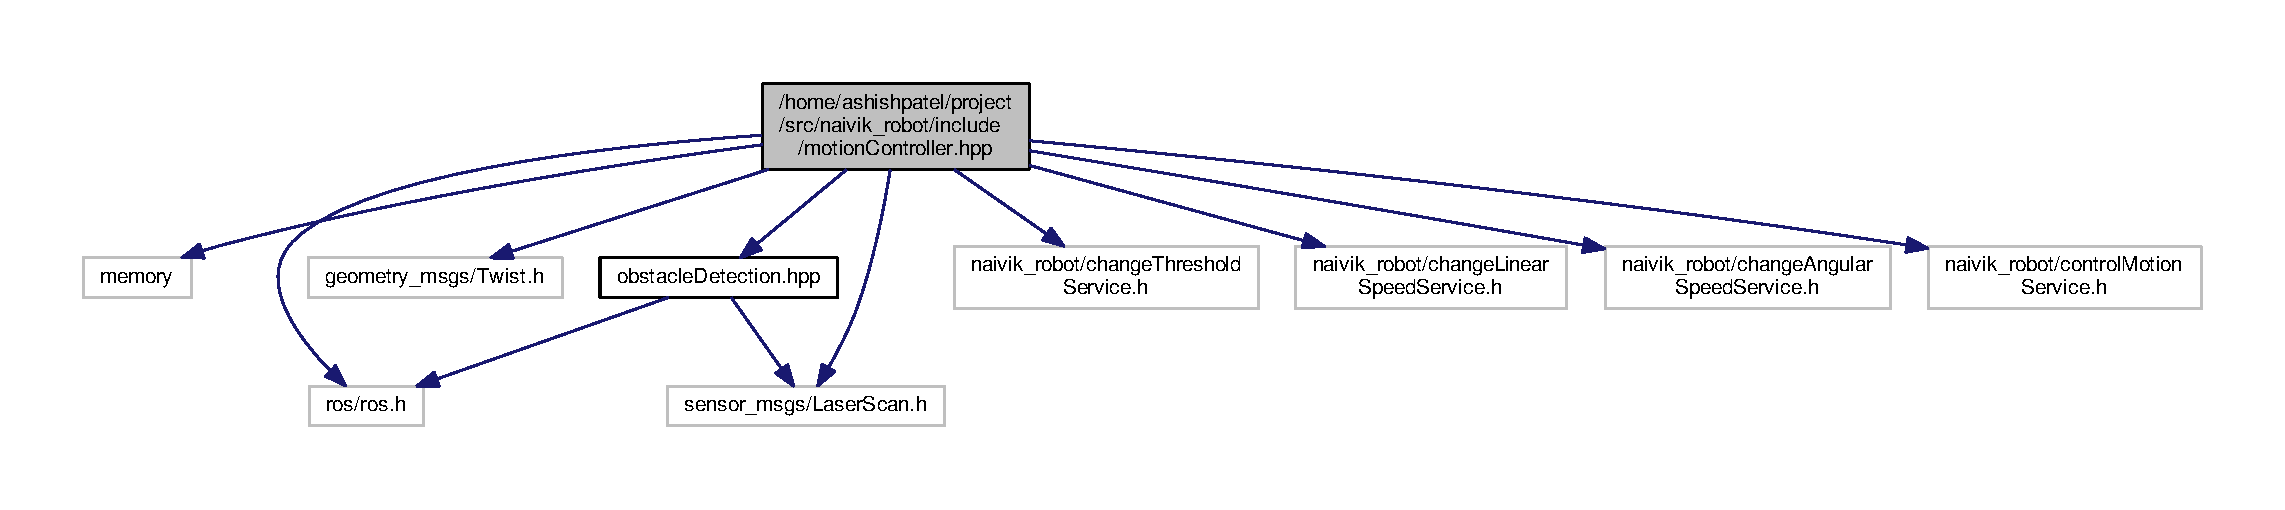
\includegraphics[width=350pt]{motionController_8hpp__incl}
\end{center}
\end{figure}
This graph shows which files directly or indirectly include this file\+:
\nopagebreak
\begin{figure}[H]
\begin{center}
\leavevmode
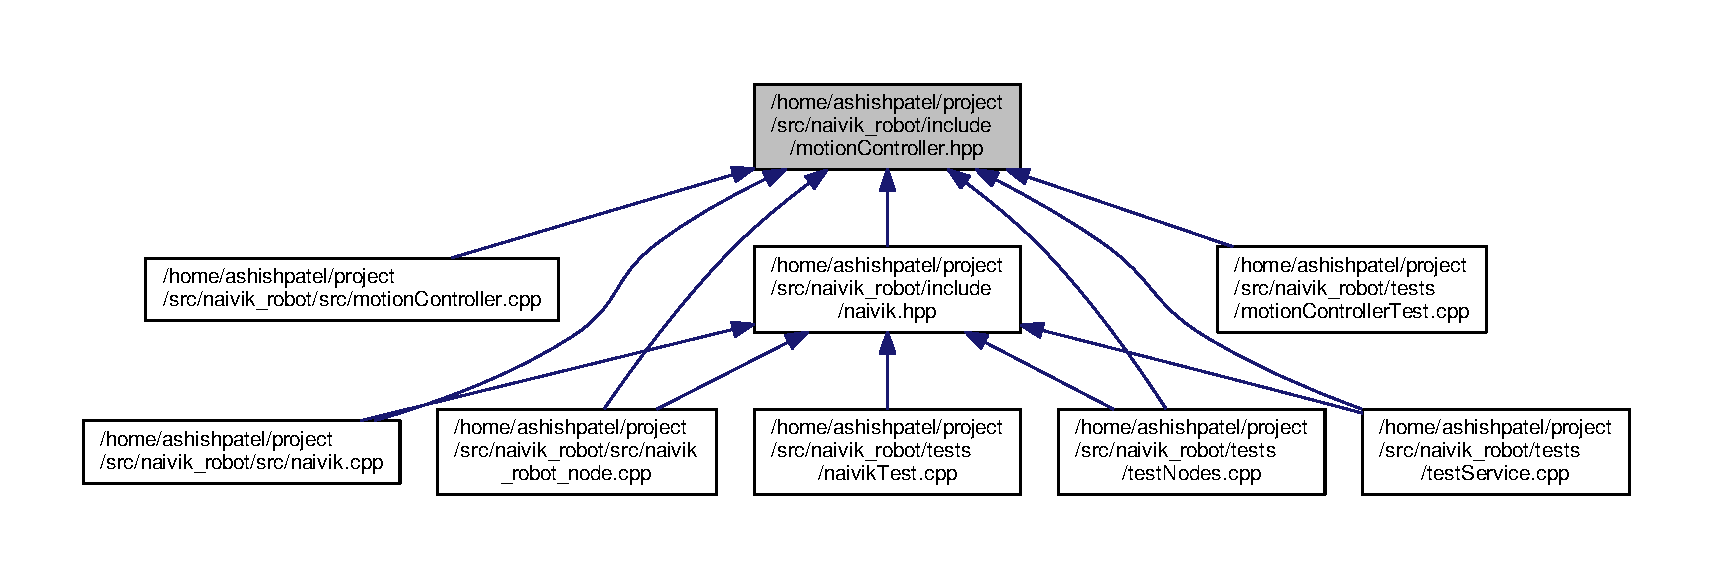
\includegraphics[width=350pt]{motionController_8hpp__dep__incl}
\end{center}
\end{figure}
\subsection*{Classes}
\begin{DoxyCompactItemize}
\item 
class \hyperlink{classMotionController}{Motion\+Controller}
\begin{DoxyCompactList}\small\item\em \hyperlink{classMotionController}{Motion\+Controller} class determine\textquotesingle{}s robot control actions. R\+OS doesn\textquotesingle{}t provide any controller, thus we need to design our own based on the requirement that we have. \end{DoxyCompactList}\end{DoxyCompactItemize}


\subsection{Detailed Description}
\hyperlink{classMotionController}{Motion\+Controller} class header file. 

M\+IT License

Copyright (c) 2018 Ashish Patel

Permission is hereby granted, free of charge, to any person obtaining a copy of this software and associated documentation files (the \char`\"{}\+Software\char`\"{}), to deal in the Software without restriction, including without limitation the rights to use, copy, modify, merge, publish, distribute, sublicense, and/or sell copies of the Software, and to permit persons to whom the Software is furnished to do so, subject to the following conditions\+:

The above copyright notice and this permission notice shall be included in all copies or substantial portions of the Software.

T\+HE S\+O\+F\+T\+W\+A\+RE IS P\+R\+O\+V\+I\+D\+ED \char`\"{}\+A\+S I\+S\char`\"{}, W\+I\+T\+H\+O\+UT W\+A\+R\+R\+A\+N\+TY OF A\+NY K\+I\+ND, E\+X\+P\+R\+E\+SS OR I\+M\+P\+L\+I\+ED, I\+N\+C\+L\+U\+D\+I\+NG B\+UT N\+OT L\+I\+M\+I\+T\+ED TO T\+HE W\+A\+R\+R\+A\+N\+T\+I\+ES OF M\+E\+R\+C\+H\+A\+N\+T\+A\+B\+I\+L\+I\+TY, F\+I\+T\+N\+E\+SS F\+OR A P\+A\+R\+T\+I\+C\+U\+L\+AR P\+U\+R\+P\+O\+SE A\+ND N\+O\+N\+I\+N\+F\+R\+I\+N\+G\+E\+M\+E\+NT. IN NO E\+V\+E\+NT S\+H\+A\+LL T\+HE A\+U\+T\+H\+O\+RS OR C\+O\+P\+Y\+R\+I\+G\+HT H\+O\+L\+D\+E\+RS BE L\+I\+A\+B\+LE F\+OR A\+NY C\+L\+A\+IM, D\+A\+M\+A\+G\+ES OR O\+T\+H\+ER L\+I\+A\+B\+I\+L\+I\+TY, W\+H\+E\+T\+H\+ER IN AN A\+C\+T\+I\+ON OF C\+O\+N\+T\+R\+A\+CT, T\+O\+RT OR O\+T\+H\+E\+R\+W\+I\+SE, A\+R\+I\+S\+I\+NG F\+R\+OM, O\+UT OF OR IN C\+O\+N\+N\+E\+C\+T\+I\+ON W\+I\+TH T\+HE S\+O\+F\+T\+W\+A\+RE OR T\+HE U\+SE OR O\+T\+H\+ER D\+E\+A\+L\+I\+N\+GS IN T\+HE S\+O\+F\+T\+W\+A\+RE.

\begin{DoxyVersion}{Version}
0.\+1 
\end{DoxyVersion}
\begin{DoxyAuthor}{Author}
Ashish Patel 
\end{DoxyAuthor}
\begin{DoxyDate}{Date}
12-\/15-\/2018 
\end{DoxyDate}

\hypertarget{naivik_8hpp}{}\section{/home/ashishpatel/project/src/naivik\+\_\+robot/include/naivik.hpp File Reference}
\label{naivik_8hpp}\index{/home/ashishpatel/project/src/naivik\+\_\+robot/include/naivik.\+hpp@{/home/ashishpatel/project/src/naivik\+\_\+robot/include/naivik.\+hpp}}


\hyperlink{classNaivik}{Naivik} class header file.  


{\ttfamily \#include $<$memory$>$}\\*
{\ttfamily \#include \char`\"{}ros/ros.\+h\char`\"{}}\\*
{\ttfamily \#include \char`\"{}sensor\+\_\+msgs/\+Laser\+Scan.\+h\char`\"{}}\\*
{\ttfamily \#include \char`\"{}geometry\+\_\+msgs/\+Twist.\+h\char`\"{}}\\*
{\ttfamily \#include \char`\"{}sensor\+\_\+msgs/\+Image.\+h\char`\"{}}\\*
{\ttfamily \#include \char`\"{}motion\+Controller.\+hpp\char`\"{}}\\*
{\ttfamily \#include \char`\"{}camera.\+hpp\char`\"{}}\\*
Include dependency graph for naivik.\+hpp\+:
\nopagebreak
\begin{figure}[H]
\begin{center}
\leavevmode
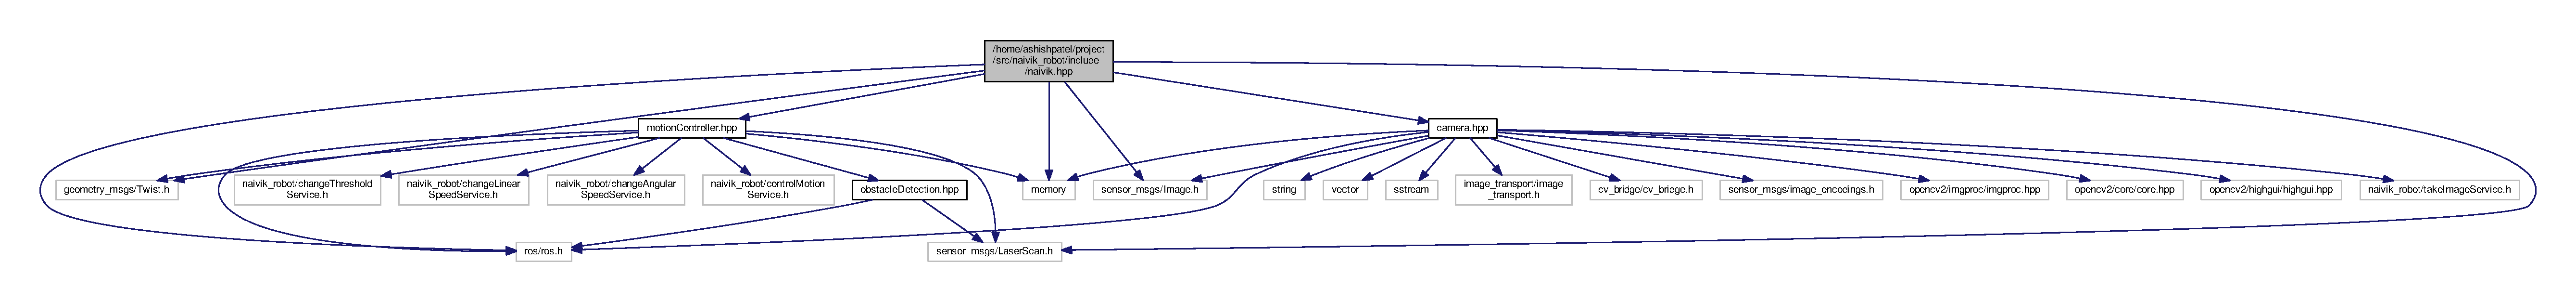
\includegraphics[width=350pt]{naivik_8hpp__incl}
\end{center}
\end{figure}
This graph shows which files directly or indirectly include this file\+:
\nopagebreak
\begin{figure}[H]
\begin{center}
\leavevmode
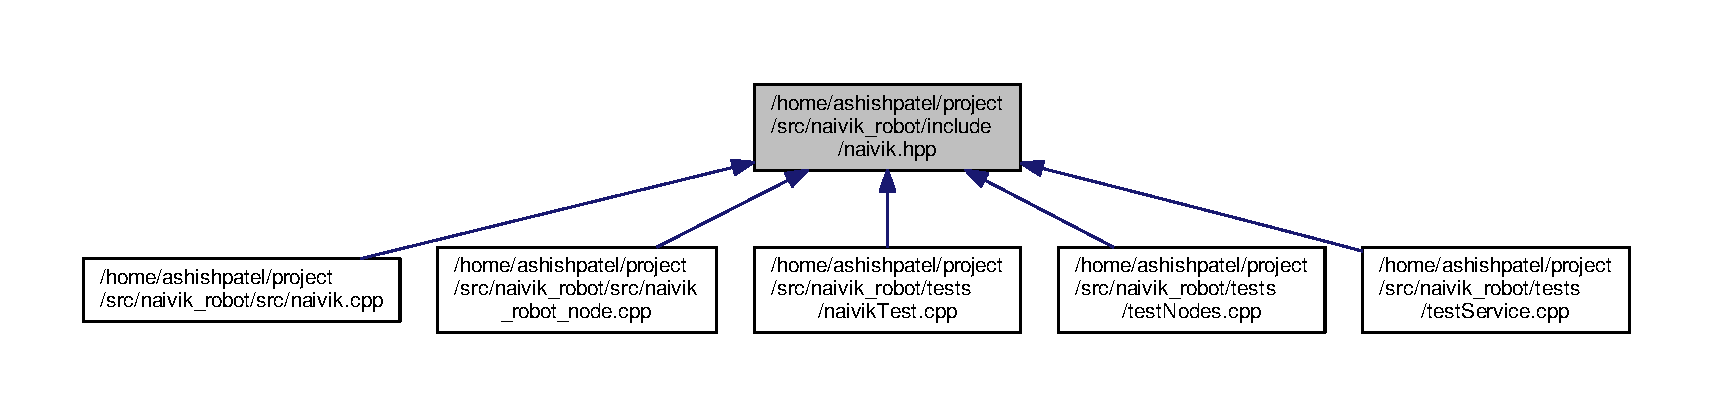
\includegraphics[width=350pt]{naivik_8hpp__dep__incl}
\end{center}
\end{figure}
\subsection*{Classes}
\begin{DoxyCompactItemize}
\item 
class \hyperlink{classNaivik}{Naivik}
\begin{DoxyCompactList}\small\item\em \hyperlink{classNaivik}{Naivik} class handles the camera and motion controller interactions of the robot. \end{DoxyCompactList}\end{DoxyCompactItemize}


\subsection{Detailed Description}
\hyperlink{classNaivik}{Naivik} class header file. 

M\+IT License

Copyright (c) 2018 Ashish Patel

Permission is hereby granted, free of charge, to any person obtaining a copy of this software and associated documentation files (the \char`\"{}\+Software\char`\"{}), to deal in the Software without restriction, including without limitation the rights to use, copy, modify, merge, publish, distribute, sublicense, and/or sell copies of the Software, and to permit persons to whom the Software is furnished to do so, subject to the following conditions\+:

The above copyright notice and this permission notice shall be included in all copies or substantial portions of the Software.

T\+HE S\+O\+F\+T\+W\+A\+RE IS P\+R\+O\+V\+I\+D\+ED \char`\"{}\+A\+S I\+S\char`\"{}, W\+I\+T\+H\+O\+UT W\+A\+R\+R\+A\+N\+TY OF A\+NY K\+I\+ND, E\+X\+P\+R\+E\+SS OR I\+M\+P\+L\+I\+ED, I\+N\+C\+L\+U\+D\+I\+NG B\+UT N\+OT L\+I\+M\+I\+T\+ED TO T\+HE W\+A\+R\+R\+A\+N\+T\+I\+ES OF M\+E\+R\+C\+H\+A\+N\+T\+A\+B\+I\+L\+I\+TY, F\+I\+T\+N\+E\+SS F\+OR A P\+A\+R\+T\+I\+C\+U\+L\+AR P\+U\+R\+P\+O\+SE A\+ND N\+O\+N\+I\+N\+F\+R\+I\+N\+G\+E\+M\+E\+NT. IN NO E\+V\+E\+NT S\+H\+A\+LL T\+HE A\+U\+T\+H\+O\+RS OR C\+O\+P\+Y\+R\+I\+G\+HT H\+O\+L\+D\+E\+RS BE L\+I\+A\+B\+LE F\+OR A\+NY C\+L\+A\+IM, D\+A\+M\+A\+G\+ES OR O\+T\+H\+ER L\+I\+A\+B\+I\+L\+I\+TY, W\+H\+E\+T\+H\+ER IN AN A\+C\+T\+I\+ON OF C\+O\+N\+T\+R\+A\+CT, T\+O\+RT OR O\+T\+H\+E\+R\+W\+I\+SE, A\+R\+I\+S\+I\+NG F\+R\+OM, O\+UT OF OR IN C\+O\+N\+N\+E\+C\+T\+I\+ON W\+I\+TH T\+HE S\+O\+F\+T\+W\+A\+RE OR T\+HE U\+SE OR O\+T\+H\+ER D\+E\+A\+L\+I\+N\+GS IN T\+HE S\+O\+F\+T\+W\+A\+RE.

\begin{DoxyVersion}{Version}
0.\+1 
\end{DoxyVersion}
\begin{DoxyAuthor}{Author}
Ashish Patel 
\end{DoxyAuthor}
\begin{DoxyDate}{Date}
12-\/15-\/2018 
\end{DoxyDate}

\hypertarget{obstacleDetection_8hpp}{}\section{/home/ashishpatel/project/src/naivik\+\_\+robot/include/obstacle\+Detection.hpp File Reference}
\label{obstacleDetection_8hpp}\index{/home/ashishpatel/project/src/naivik\+\_\+robot/include/obstacle\+Detection.\+hpp@{/home/ashishpatel/project/src/naivik\+\_\+robot/include/obstacle\+Detection.\+hpp}}


\hyperlink{classObstacleDetection}{Obstacle\+Detection} class header file.  


{\ttfamily \#include \char`\"{}ros/ros.\+h\char`\"{}}\\*
{\ttfamily \#include \char`\"{}sensor\+\_\+msgs/\+Laser\+Scan.\+h\char`\"{}}\\*
Include dependency graph for obstacle\+Detection.\+hpp\+:
\nopagebreak
\begin{figure}[H]
\begin{center}
\leavevmode
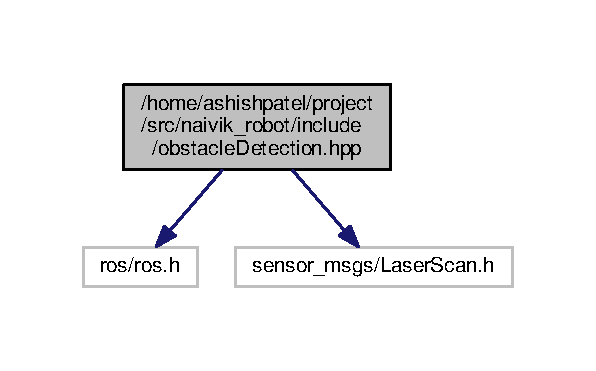
\includegraphics[width=286pt]{obstacleDetection_8hpp__incl}
\end{center}
\end{figure}
This graph shows which files directly or indirectly include this file\+:
\nopagebreak
\begin{figure}[H]
\begin{center}
\leavevmode
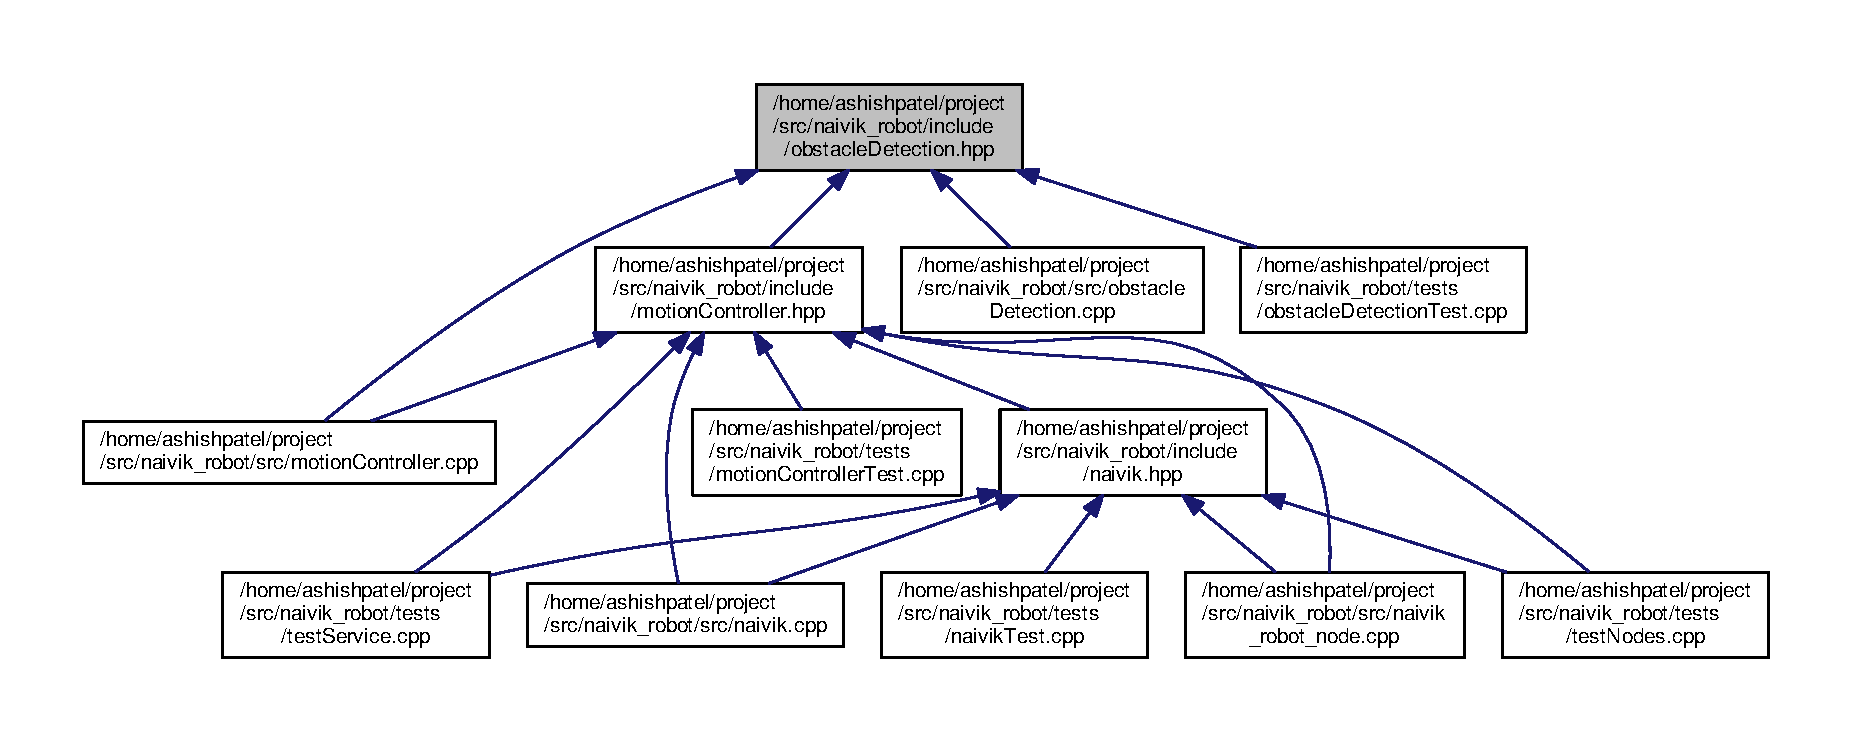
\includegraphics[width=350pt]{obstacleDetection_8hpp__dep__incl}
\end{center}
\end{figure}
\subsection*{Classes}
\begin{DoxyCompactItemize}
\item 
class \hyperlink{classObstacleDetection}{Obstacle\+Detection}
\begin{DoxyCompactList}\small\item\em \hyperlink{classObstacleDetection}{Obstacle\+Detection} class handles determining if the vehicle is going to collide using laser scans data. \end{DoxyCompactList}\end{DoxyCompactItemize}


\subsection{Detailed Description}
\hyperlink{classObstacleDetection}{Obstacle\+Detection} class header file. 

M\+IT License

Copyright (c) 2018 Ashish Patel

Permission is hereby granted, free of charge, to any person obtaining a copy of this software and associated documentation files (the \char`\"{}\+Software\char`\"{}), to deal in the Software without restriction, including without limitation the rights to use, copy, modify, merge, publish, distribute, sublicense, and/or sell copies of the Software, and to permit persons to whom the Software is furnished to do so, subject to the following conditions\+:

The above copyright notice and this permission notice shall be included in all copies or substantial portions of the Software.

T\+HE S\+O\+F\+T\+W\+A\+RE IS P\+R\+O\+V\+I\+D\+ED \char`\"{}\+A\+S I\+S\char`\"{}, W\+I\+T\+H\+O\+UT W\+A\+R\+R\+A\+N\+TY OF A\+NY K\+I\+ND, E\+X\+P\+R\+E\+SS OR I\+M\+P\+L\+I\+ED, I\+N\+C\+L\+U\+D\+I\+NG B\+UT N\+OT L\+I\+M\+I\+T\+ED TO T\+HE W\+A\+R\+R\+A\+N\+T\+I\+ES OF M\+E\+R\+C\+H\+A\+N\+T\+A\+B\+I\+L\+I\+TY, F\+I\+T\+N\+E\+SS F\+OR A P\+A\+R\+T\+I\+C\+U\+L\+AR P\+U\+R\+P\+O\+SE A\+ND N\+O\+N\+I\+N\+F\+R\+I\+N\+G\+E\+M\+E\+NT. IN NO E\+V\+E\+NT S\+H\+A\+LL T\+HE A\+U\+T\+H\+O\+RS OR C\+O\+P\+Y\+R\+I\+G\+HT H\+O\+L\+D\+E\+RS BE L\+I\+A\+B\+LE F\+OR A\+NY C\+L\+A\+IM, D\+A\+M\+A\+G\+ES OR O\+T\+H\+ER L\+I\+A\+B\+I\+L\+I\+TY, W\+H\+E\+T\+H\+ER IN AN A\+C\+T\+I\+ON OF C\+O\+N\+T\+R\+A\+CT, T\+O\+RT OR O\+T\+H\+E\+R\+W\+I\+SE, A\+R\+I\+S\+I\+NG F\+R\+OM, O\+UT OF OR IN C\+O\+N\+N\+E\+C\+T\+I\+ON W\+I\+TH T\+HE S\+O\+F\+T\+W\+A\+RE OR T\+HE U\+SE OR O\+T\+H\+ER D\+E\+A\+L\+I\+N\+GS IN T\+HE S\+O\+F\+T\+W\+A\+RE.

\begin{DoxyVersion}{Version}
0.\+1 
\end{DoxyVersion}
\begin{DoxyAuthor}{Author}
Ashish Patel 
\end{DoxyAuthor}
\begin{DoxyDate}{Date}
12-\/15-\/2018 
\end{DoxyDate}

\hypertarget{camera_8cpp}{}\section{/home/ashishpatel/project/src/naivik\+\_\+robot/src/camera.cpp File Reference}
\label{camera_8cpp}\index{/home/ashishpatel/project/src/naivik\+\_\+robot/src/camera.\+cpp@{/home/ashishpatel/project/src/naivik\+\_\+robot/src/camera.\+cpp}}


\hyperlink{classCamera}{Camera} class implementation file.  


{\ttfamily \#include $<$memory$>$}\\*
{\ttfamily \#include $<$string$>$}\\*
{\ttfamily \#include $<$vector$>$}\\*
{\ttfamily \#include $<$sstream$>$}\\*
{\ttfamily \#include \char`\"{}ros/ros.\+h\char`\"{}}\\*
{\ttfamily \#include \char`\"{}image\+\_\+transport/image\+\_\+transport.\+h\char`\"{}}\\*
{\ttfamily \#include \char`\"{}cv\+\_\+bridge/cv\+\_\+bridge.\+h\char`\"{}}\\*
{\ttfamily \#include \char`\"{}sensor\+\_\+msgs/\+Image.\+h\char`\"{}}\\*
{\ttfamily \#include \char`\"{}sensor\+\_\+msgs/image\+\_\+encodings.\+h\char`\"{}}\\*
{\ttfamily \#include \char`\"{}opencv2/imgproc/imgproc.\+hpp\char`\"{}}\\*
{\ttfamily \#include \char`\"{}opencv2/core/core.\+hpp\char`\"{}}\\*
{\ttfamily \#include \char`\"{}opencv2/highgui/highgui.\+hpp\char`\"{}}\\*
{\ttfamily \#include \char`\"{}naivik\+\_\+robot/take\+Image\+Service.\+h\char`\"{}}\\*
{\ttfamily \#include \char`\"{}camera.\+hpp\char`\"{}}\\*
Include dependency graph for camera.\+cpp\+:
\nopagebreak
\begin{figure}[H]
\begin{center}
\leavevmode
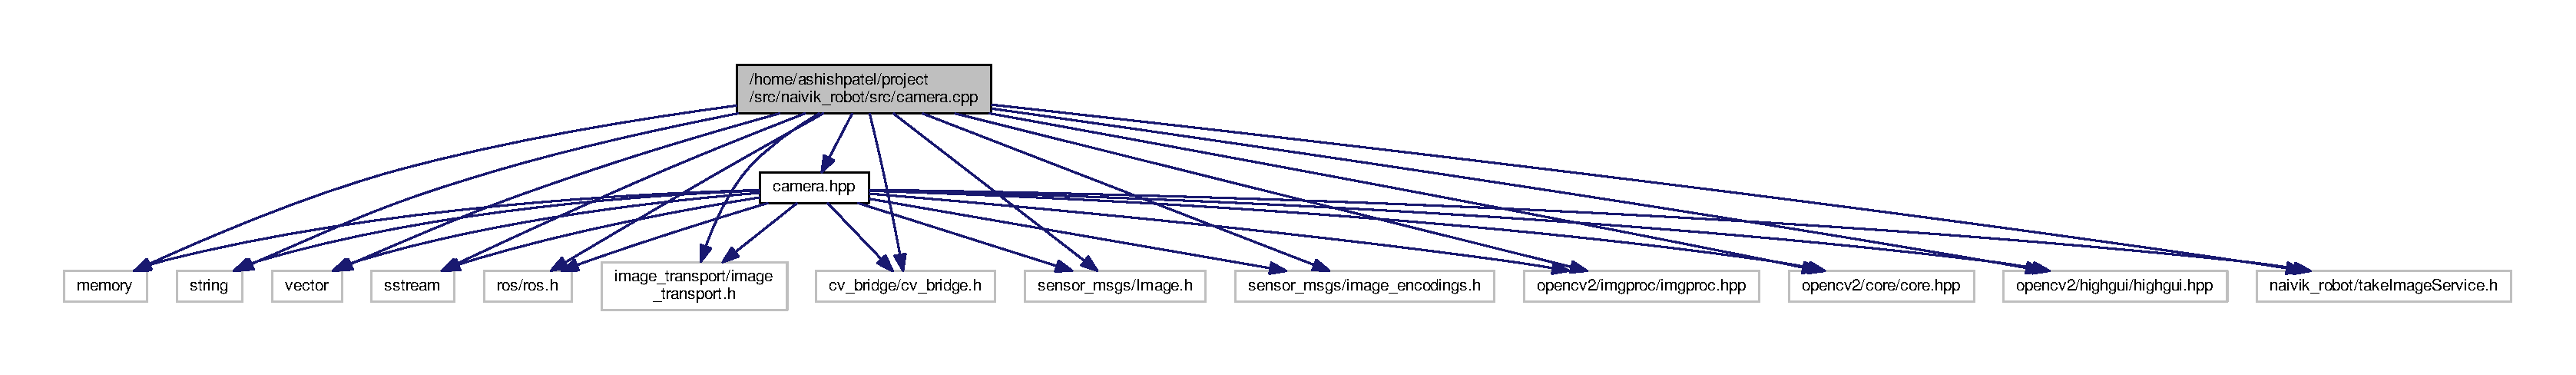
\includegraphics[width=350pt]{camera_8cpp__incl}
\end{center}
\end{figure}


\subsection{Detailed Description}
\hyperlink{classCamera}{Camera} class implementation file. 

M\+IT License

Copyright (c) 2018 Ashish Patel

Permission is hereby granted, free of charge, to any person obtaining a copy of this software and associated documentation files (the \char`\"{}\+Software\char`\"{}), to deal in the Software without restriction, including without limitation the rights to use, copy, modify, merge, publish, distribute, sublicense, and/or sell copies of the Software, and to permit persons to whom the Software is furnished to do so, subject to the following conditions\+:

The above copyright notice and this permission notice shall be included in all copies or substantial portions of the Software.

T\+HE S\+O\+F\+T\+W\+A\+RE IS P\+R\+O\+V\+I\+D\+ED \char`\"{}\+A\+S I\+S\char`\"{}, W\+I\+T\+H\+O\+UT W\+A\+R\+R\+A\+N\+TY OF A\+NY K\+I\+ND, E\+X\+P\+R\+E\+SS OR I\+M\+P\+L\+I\+ED, I\+N\+C\+L\+U\+D\+I\+NG B\+UT N\+OT L\+I\+M\+I\+T\+ED TO T\+HE W\+A\+R\+R\+A\+N\+T\+I\+ES OF M\+E\+R\+C\+H\+A\+N\+T\+A\+B\+I\+L\+I\+TY, F\+I\+T\+N\+E\+SS F\+OR A P\+A\+R\+T\+I\+C\+U\+L\+AR P\+U\+R\+P\+O\+SE A\+ND N\+O\+N\+I\+N\+F\+R\+I\+N\+G\+E\+M\+E\+NT. IN NO E\+V\+E\+NT S\+H\+A\+LL T\+HE A\+U\+T\+H\+O\+RS OR C\+O\+P\+Y\+R\+I\+G\+HT H\+O\+L\+D\+E\+RS BE L\+I\+A\+B\+LE F\+OR A\+NY C\+L\+A\+IM, D\+A\+M\+A\+G\+ES OR O\+T\+H\+ER L\+I\+A\+B\+I\+L\+I\+TY, W\+H\+E\+T\+H\+ER IN AN A\+C\+T\+I\+ON OF C\+O\+N\+T\+R\+A\+CT, T\+O\+RT OR O\+T\+H\+E\+R\+W\+I\+SE, A\+R\+I\+S\+I\+NG F\+R\+OM, O\+UT OF OR IN C\+O\+N\+N\+E\+C\+T\+I\+ON W\+I\+TH T\+HE S\+O\+F\+T\+W\+A\+RE OR T\+HE U\+SE OR O\+T\+H\+ER D\+E\+A\+L\+I\+N\+GS IN T\+HE S\+O\+F\+T\+W\+A\+RE.

\begin{DoxyVersion}{Version}
0.\+1 
\end{DoxyVersion}
\begin{DoxyAuthor}{Author}
Ashish Patel 
\end{DoxyAuthor}
\begin{DoxyDate}{Date}
12-\/15-\/2018 
\end{DoxyDate}

\hypertarget{motionController_8cpp}{}\section{/home/ashishpatel/project/src/naivik\+\_\+robot/src/motion\+Controller.cpp File Reference}
\label{motionController_8cpp}\index{/home/ashishpatel/project/src/naivik\+\_\+robot/src/motion\+Controller.\+cpp@{/home/ashishpatel/project/src/naivik\+\_\+robot/src/motion\+Controller.\+cpp}}
{\ttfamily \#include $<$memory$>$}\\*
{\ttfamily \#include \char`\"{}ros/ros.\+h\char`\"{}}\\*
{\ttfamily \#include \char`\"{}geometry\+\_\+msgs/\+Twist.\+h\char`\"{}}\\*
{\ttfamily \#include \char`\"{}sensor\+\_\+msgs/\+Laser\+Scan.\+h\char`\"{}}\\*
{\ttfamily \#include \char`\"{}motion\+Controller.\+hpp\char`\"{}}\\*
{\ttfamily \#include \char`\"{}obstacle\+Detection.\+hpp\char`\"{}}\\*
{\ttfamily \#include \char`\"{}naivik\+\_\+robot/change\+Threshold\+Service.\+h\char`\"{}}\\*
{\ttfamily \#include \char`\"{}naivik\+\_\+robot/change\+Linear\+Speed\+Service.\+h\char`\"{}}\\*
{\ttfamily \#include \char`\"{}naivik\+\_\+robot/change\+Angular\+Speed\+Service.\+h\char`\"{}}\\*
{\ttfamily \#include \char`\"{}naivik\+\_\+robot/control\+Motion\+Service.\+h\char`\"{}}\\*
Include dependency graph for motion\+Controller.\+cpp\+:
\nopagebreak
\begin{figure}[H]
\begin{center}
\leavevmode
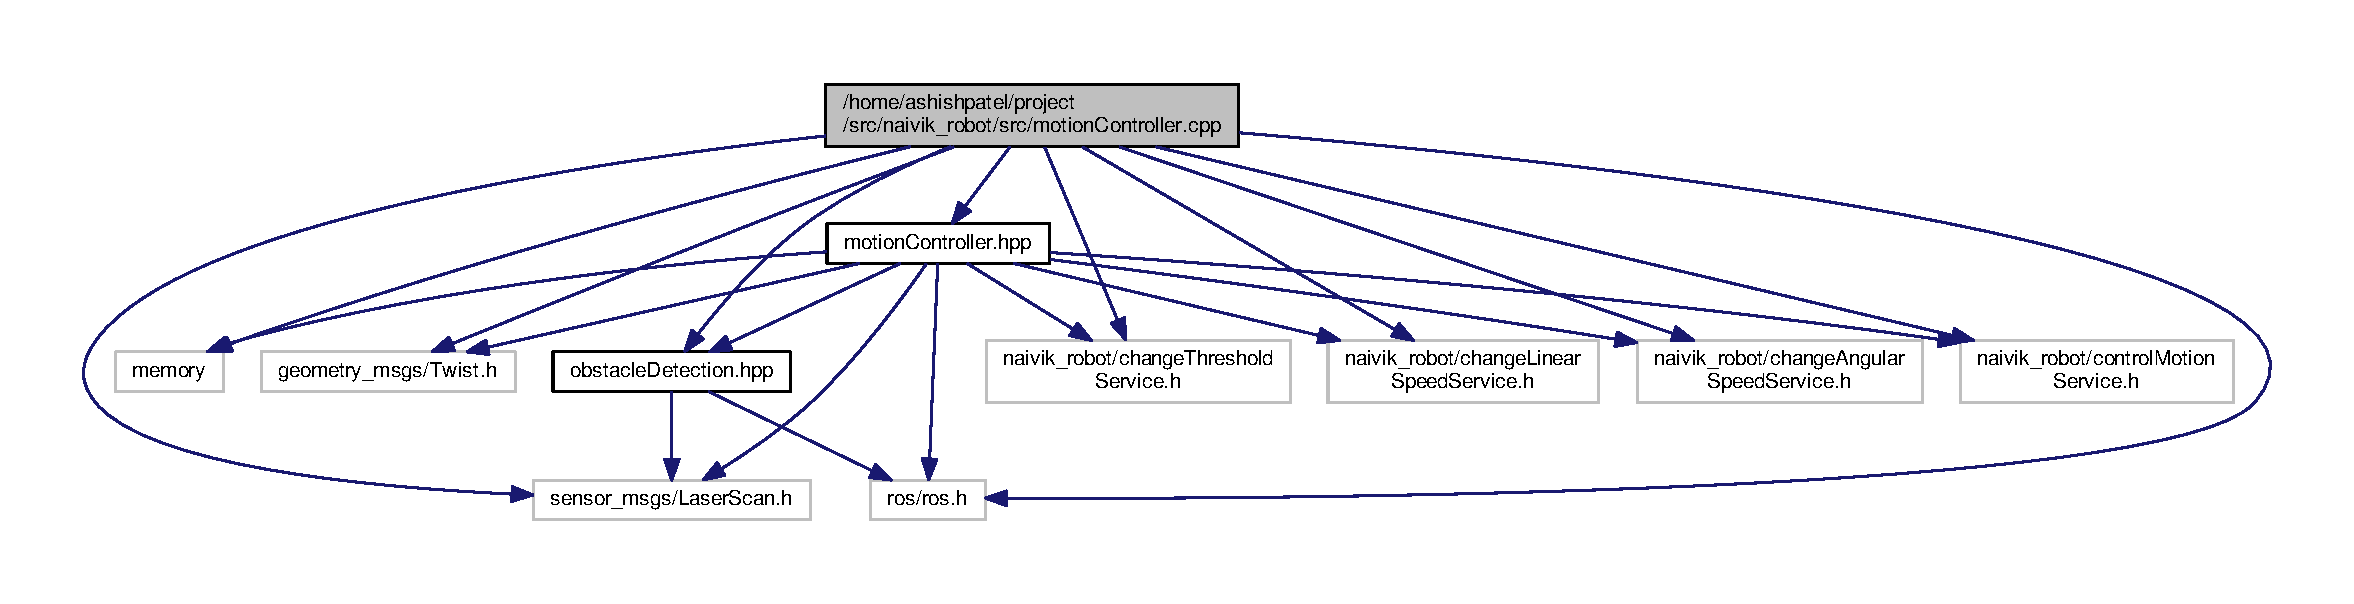
\includegraphics[width=350pt]{motionController_8cpp__incl}
\end{center}
\end{figure}

\hypertarget{naivik_8cpp}{}\section{/home/ashishpatel/project/src/naivik\+\_\+robot/src/naivik.cpp File Reference}
\label{naivik_8cpp}\index{/home/ashishpatel/project/src/naivik\+\_\+robot/src/naivik.\+cpp@{/home/ashishpatel/project/src/naivik\+\_\+robot/src/naivik.\+cpp}}


\hyperlink{classNaivik}{Naivik} class implementation file.  


{\ttfamily \#include $<$memory$>$}\\*
{\ttfamily \#include \char`\"{}ros/ros.\+h\char`\"{}}\\*
{\ttfamily \#include \char`\"{}sensor\+\_\+msgs/\+Laser\+Scan.\+h\char`\"{}}\\*
{\ttfamily \#include \char`\"{}geometry\+\_\+msgs/\+Twist.\+h\char`\"{}}\\*
{\ttfamily \#include \char`\"{}sensor\+\_\+msgs/\+Image.\+h\char`\"{}}\\*
{\ttfamily \#include \char`\"{}naivik.\+hpp\char`\"{}}\\*
{\ttfamily \#include \char`\"{}motion\+Controller.\+hpp\char`\"{}}\\*
{\ttfamily \#include \char`\"{}camera.\+hpp\char`\"{}}\\*
Include dependency graph for naivik.\+cpp\+:
\nopagebreak
\begin{figure}[H]
\begin{center}
\leavevmode
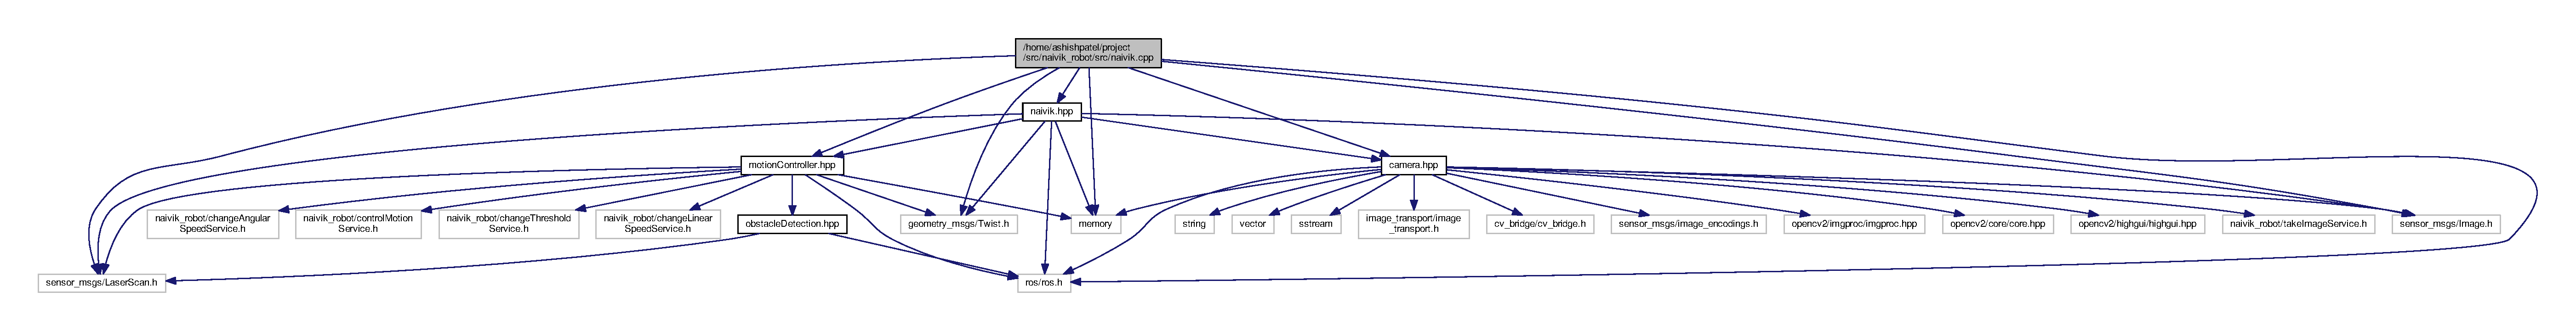
\includegraphics[width=350pt]{naivik_8cpp__incl}
\end{center}
\end{figure}


\subsection{Detailed Description}
\hyperlink{classNaivik}{Naivik} class implementation file. 

M\+IT License

Copyright (c) 2018 Ashish Patel

Permission is hereby granted, free of charge, to any person obtaining a copy of this software and associated documentation files (the \char`\"{}\+Software\char`\"{}), to deal in the Software without restriction, including without limitation the rights to use, copy, modify, merge, publish, distribute, sublicense, and/or sell copies of the Software, and to permit persons to whom the Software is furnished to do so, subject to the following conditions\+:

The above copyright notice and this permission notice shall be included in all copies or substantial portions of the Software.

T\+HE S\+O\+F\+T\+W\+A\+RE IS P\+R\+O\+V\+I\+D\+ED \char`\"{}\+A\+S I\+S\char`\"{}, W\+I\+T\+H\+O\+UT W\+A\+R\+R\+A\+N\+TY OF A\+NY K\+I\+ND, E\+X\+P\+R\+E\+SS OR I\+M\+P\+L\+I\+ED, I\+N\+C\+L\+U\+D\+I\+NG B\+UT N\+OT L\+I\+M\+I\+T\+ED TO T\+HE W\+A\+R\+R\+A\+N\+T\+I\+ES OF M\+E\+R\+C\+H\+A\+N\+T\+A\+B\+I\+L\+I\+TY, F\+I\+T\+N\+E\+SS F\+OR A P\+A\+R\+T\+I\+C\+U\+L\+AR P\+U\+R\+P\+O\+SE A\+ND N\+O\+N\+I\+N\+F\+R\+I\+N\+G\+E\+M\+E\+NT. IN NO E\+V\+E\+NT S\+H\+A\+LL T\+HE A\+U\+T\+H\+O\+RS OR C\+O\+P\+Y\+R\+I\+G\+HT H\+O\+L\+D\+E\+RS BE L\+I\+A\+B\+LE F\+OR A\+NY C\+L\+A\+IM, D\+A\+M\+A\+G\+ES OR O\+T\+H\+ER L\+I\+A\+B\+I\+L\+I\+TY, W\+H\+E\+T\+H\+ER IN AN A\+C\+T\+I\+ON OF C\+O\+N\+T\+R\+A\+CT, T\+O\+RT OR O\+T\+H\+E\+R\+W\+I\+SE, A\+R\+I\+S\+I\+NG F\+R\+OM, O\+UT OF OR IN C\+O\+N\+N\+E\+C\+T\+I\+ON W\+I\+TH T\+HE S\+O\+F\+T\+W\+A\+RE OR T\+HE U\+SE OR O\+T\+H\+ER D\+E\+A\+L\+I\+N\+GS IN T\+HE S\+O\+F\+T\+W\+A\+RE.

\begin{DoxyVersion}{Version}
0.\+1 
\end{DoxyVersion}
\begin{DoxyAuthor}{Author}
Ashish Patel 
\end{DoxyAuthor}
\begin{DoxyDate}{Date}
12-\/15-\/2018 
\end{DoxyDate}

\hypertarget{naivik__robot__node_8cpp}{}\section{/home/ashishpatel/project/src/naivik\+\_\+robot/src/naivik\+\_\+robot\+\_\+node.cpp File Reference}
\label{naivik__robot__node_8cpp}\index{/home/ashishpatel/project/src/naivik\+\_\+robot/src/naivik\+\_\+robot\+\_\+node.\+cpp@{/home/ashishpatel/project/src/naivik\+\_\+robot/src/naivik\+\_\+robot\+\_\+node.\+cpp}}


R\+OS package entry point.  


{\ttfamily \#include $<$memory$>$}\\*
{\ttfamily \#include \char`\"{}ros/ros.\+h\char`\"{}}\\*
{\ttfamily \#include \char`\"{}sensor\+\_\+msgs/\+Laser\+Scan.\+h\char`\"{}}\\*
{\ttfamily \#include \char`\"{}geometry\+\_\+msgs/\+Twist.\+h\char`\"{}}\\*
{\ttfamily \#include \char`\"{}sensor\+\_\+msgs/\+Image.\+h\char`\"{}}\\*
{\ttfamily \#include \char`\"{}naivik.\+hpp\char`\"{}}\\*
{\ttfamily \#include \char`\"{}motion\+Controller.\+hpp\char`\"{}}\\*
{\ttfamily \#include \char`\"{}camera.\+hpp\char`\"{}}\\*
Include dependency graph for naivik\+\_\+robot\+\_\+node.\+cpp\+:
\nopagebreak
\begin{figure}[H]
\begin{center}
\leavevmode
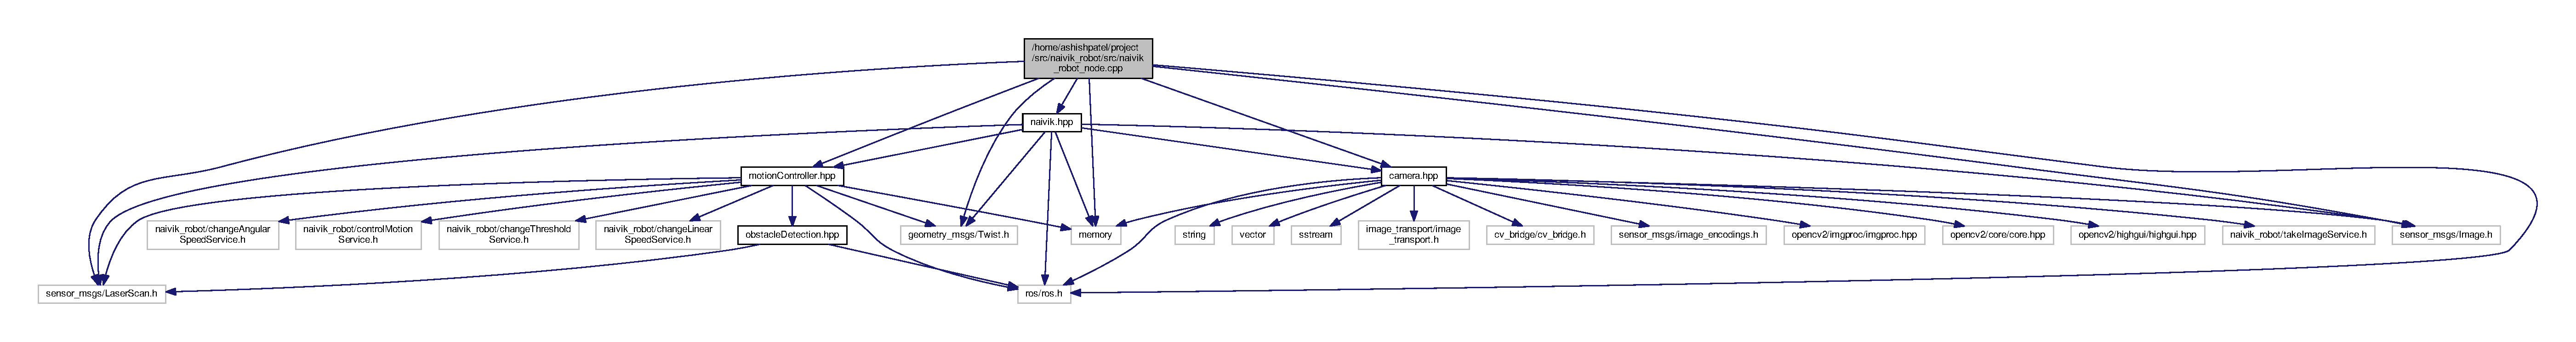
\includegraphics[width=350pt]{naivik__robot__node_8cpp__incl}
\end{center}
\end{figure}
\subsection*{Functions}
\begin{DoxyCompactItemize}
\item 
int \hyperlink{naivik__robot__node_8cpp_a3c04138a5bfe5d72780bb7e82a18e627}{main} (int argc, char $\ast$$\ast$argv)
\end{DoxyCompactItemize}


\subsection{Detailed Description}
R\+OS package entry point. 

M\+IT License

Copyright (c) 2018 Ashish Patel

Permission is hereby granted, free of charge, to any person obtaining a copy of this software and associated documentation files (the \char`\"{}\+Software\char`\"{}), to deal in the Software without restriction, including without limitation the rights to use, copy, modify, merge, publish, distribute, sublicense, and/or sell copies of the Software, and to permit persons to whom the Software is furnished to do so, subject to the following conditions\+:

The above copyright notice and this permission notice shall be included in all copies or substantial portions of the Software.

T\+HE S\+O\+F\+T\+W\+A\+RE IS P\+R\+O\+V\+I\+D\+ED \char`\"{}\+A\+S I\+S\char`\"{}, W\+I\+T\+H\+O\+UT W\+A\+R\+R\+A\+N\+TY OF A\+NY K\+I\+ND, E\+X\+P\+R\+E\+SS OR I\+M\+P\+L\+I\+ED, I\+N\+C\+L\+U\+D\+I\+NG B\+UT N\+OT L\+I\+M\+I\+T\+ED TO T\+HE W\+A\+R\+R\+A\+N\+T\+I\+ES OF M\+E\+R\+C\+H\+A\+N\+T\+A\+B\+I\+L\+I\+TY, F\+I\+T\+N\+E\+SS F\+OR A P\+A\+R\+T\+I\+C\+U\+L\+AR P\+U\+R\+P\+O\+SE A\+ND N\+O\+N\+I\+N\+F\+R\+I\+N\+G\+E\+M\+E\+NT. IN NO E\+V\+E\+NT S\+H\+A\+LL T\+HE A\+U\+T\+H\+O\+RS OR C\+O\+P\+Y\+R\+I\+G\+HT H\+O\+L\+D\+E\+RS BE L\+I\+A\+B\+LE F\+OR A\+NY C\+L\+A\+IM, D\+A\+M\+A\+G\+ES OR O\+T\+H\+ER L\+I\+A\+B\+I\+L\+I\+TY, W\+H\+E\+T\+H\+ER IN AN A\+C\+T\+I\+ON OF C\+O\+N\+T\+R\+A\+CT, T\+O\+RT OR O\+T\+H\+E\+R\+W\+I\+SE, A\+R\+I\+S\+I\+NG F\+R\+OM, O\+UT OF OR IN C\+O\+N\+N\+E\+C\+T\+I\+ON W\+I\+TH T\+HE S\+O\+F\+T\+W\+A\+RE OR T\+HE U\+SE OR O\+T\+H\+ER D\+E\+A\+L\+I\+N\+GS IN T\+HE S\+O\+F\+T\+W\+A\+RE.

\begin{DoxyVersion}{Version}
0.\+1 
\end{DoxyVersion}
\begin{DoxyAuthor}{Author}
Ashish Patel 
\end{DoxyAuthor}
\begin{DoxyDate}{Date}
12-\/15-\/2018 
\end{DoxyDate}


\subsection{Function Documentation}
\index{naivik\+\_\+robot\+\_\+node.\+cpp@{naivik\+\_\+robot\+\_\+node.\+cpp}!main@{main}}
\index{main@{main}!naivik\+\_\+robot\+\_\+node.\+cpp@{naivik\+\_\+robot\+\_\+node.\+cpp}}
\subsubsection[{\texorpdfstring{main(int argc, char $\ast$$\ast$argv)}{main(int argc, char **argv)}}]{\setlength{\rightskip}{0pt plus 5cm}int main (
\begin{DoxyParamCaption}
\item[{int}]{argc, }
\item[{char $\ast$$\ast$}]{argv}
\end{DoxyParamCaption}
)}\hypertarget{naivik__robot__node_8cpp_a3c04138a5bfe5d72780bb7e82a18e627}{}\label{naivik__robot__node_8cpp_a3c04138a5bfe5d72780bb7e82a18e627}

\hypertarget{obstacleDetection_8cpp}{}\section{/home/ashishpatel/project/src/naivik\+\_\+robot/src/obstacle\+Detection.cpp File Reference}
\label{obstacleDetection_8cpp}\index{/home/ashishpatel/project/src/naivik\+\_\+robot/src/obstacle\+Detection.\+cpp@{/home/ashishpatel/project/src/naivik\+\_\+robot/src/obstacle\+Detection.\+cpp}}


\hyperlink{classObstacleDetection}{Obstacle\+Detection} class header file.  


{\ttfamily \#include \char`\"{}ros/ros.\+h\char`\"{}}\\*
{\ttfamily \#include \char`\"{}sensor\+\_\+msgs/\+Laser\+Scan.\+h\char`\"{}}\\*
{\ttfamily \#include \char`\"{}obstacle\+Detection.\+hpp\char`\"{}}\\*
Include dependency graph for obstacle\+Detection.\+cpp\+:
\nopagebreak
\begin{figure}[H]
\begin{center}
\leavevmode
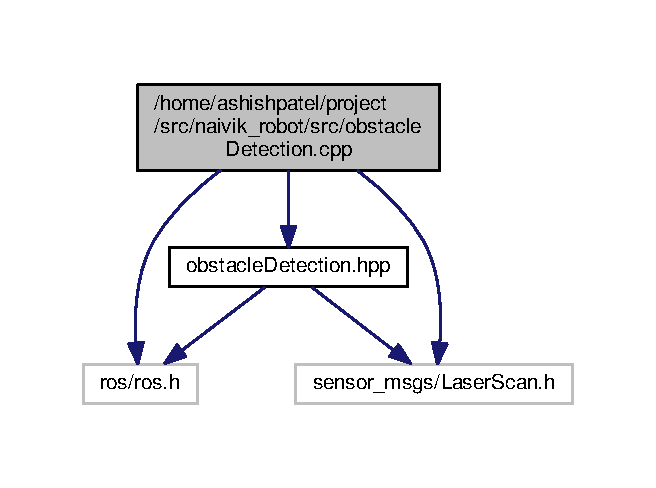
\includegraphics[width=315pt]{obstacleDetection_8cpp__incl}
\end{center}
\end{figure}


\subsection{Detailed Description}
\hyperlink{classObstacleDetection}{Obstacle\+Detection} class header file. 

M\+IT License

Copyright (c) 2018 Ashish Patel

Permission is hereby granted, free of charge, to any person obtaining a copy of this software and associated documentation files (the \char`\"{}\+Software\char`\"{}), to deal in the Software without restriction, including without limitation the rights to use, copy, modify, merge, publish, distribute, sublicense, and/or sell copies of the Software, and to permit persons to whom the Software is furnished to do so, subject to the following conditions\+:

The above copyright notice and this permission notice shall be included in all copies or substantial portions of the Software.

T\+HE S\+O\+F\+T\+W\+A\+RE IS P\+R\+O\+V\+I\+D\+ED \char`\"{}\+A\+S I\+S\char`\"{}, W\+I\+T\+H\+O\+UT W\+A\+R\+R\+A\+N\+TY OF A\+NY K\+I\+ND, E\+X\+P\+R\+E\+SS OR I\+M\+P\+L\+I\+ED, I\+N\+C\+L\+U\+D\+I\+NG B\+UT N\+OT L\+I\+M\+I\+T\+ED TO T\+HE W\+A\+R\+R\+A\+N\+T\+I\+ES OF M\+E\+R\+C\+H\+A\+N\+T\+A\+B\+I\+L\+I\+TY, F\+I\+T\+N\+E\+SS F\+OR A P\+A\+R\+T\+I\+C\+U\+L\+AR P\+U\+R\+P\+O\+SE A\+ND N\+O\+N\+I\+N\+F\+R\+I\+N\+G\+E\+M\+E\+NT. IN NO E\+V\+E\+NT S\+H\+A\+LL T\+HE A\+U\+T\+H\+O\+RS OR C\+O\+P\+Y\+R\+I\+G\+HT H\+O\+L\+D\+E\+RS BE L\+I\+A\+B\+LE F\+OR A\+NY C\+L\+A\+IM, D\+A\+M\+A\+G\+ES OR O\+T\+H\+ER L\+I\+A\+B\+I\+L\+I\+TY, W\+H\+E\+T\+H\+ER IN AN A\+C\+T\+I\+ON OF C\+O\+N\+T\+R\+A\+CT, T\+O\+RT OR O\+T\+H\+E\+R\+W\+I\+SE, A\+R\+I\+S\+I\+NG F\+R\+OM, O\+UT OF OR IN C\+O\+N\+N\+E\+C\+T\+I\+ON W\+I\+TH T\+HE S\+O\+F\+T\+W\+A\+RE OR T\+HE U\+SE OR O\+T\+H\+ER D\+E\+A\+L\+I\+N\+GS IN T\+HE S\+O\+F\+T\+W\+A\+RE.

\begin{DoxyVersion}{Version}
0.\+1 
\end{DoxyVersion}
\begin{DoxyAuthor}{Author}
Ashish Patel 
\end{DoxyAuthor}
\begin{DoxyDate}{Date}
12-\/15-\/2018 
\end{DoxyDate}

\hypertarget{cameraTest_8cpp}{}\section{/home/ashishpatel/project/src/naivik\+\_\+robot/tests/camera\+Test.cpp File Reference}
\label{cameraTest_8cpp}\index{/home/ashishpatel/project/src/naivik\+\_\+robot/tests/camera\+Test.\+cpp@{/home/ashishpatel/project/src/naivik\+\_\+robot/tests/camera\+Test.\+cpp}}


Test cases for \hyperlink{classCamera}{Camera} class.  


{\ttfamily \#include $<$gtest/gtest.\+h$>$}\\*
{\ttfamily \#include $<$memory$>$}\\*
{\ttfamily \#include \char`\"{}camera.\+hpp\char`\"{}}\\*
{\ttfamily \#include \char`\"{}ros/ros.\+h\char`\"{}}\\*
Include dependency graph for camera\+Test.\+cpp\+:
\nopagebreak
\begin{figure}[H]
\begin{center}
\leavevmode
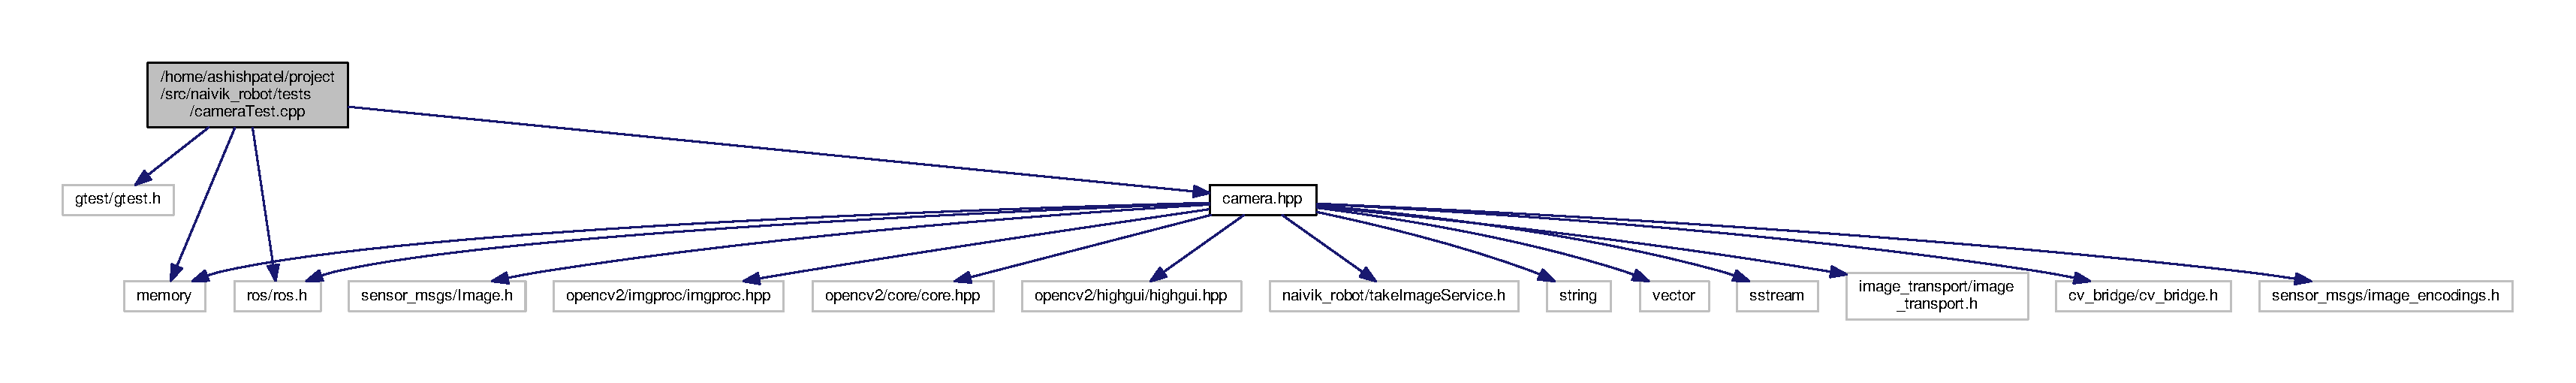
\includegraphics[width=350pt]{cameraTest_8cpp__incl}
\end{center}
\end{figure}
\subsection*{Functions}
\begin{DoxyCompactItemize}
\item 
\hyperlink{cameraTest_8cpp_ae703eea73ad1e1cc88652309be0d9be5}{T\+E\+ST} (Camera\+Test, initialization\+\_\+test)
\begin{DoxyCompactList}\small\item\em Test that should pass. \end{DoxyCompactList}\end{DoxyCompactItemize}


\subsection{Detailed Description}
Test cases for \hyperlink{classCamera}{Camera} class. 

M\+IT License

Copyright (c) 2018 Ashish Patel

Permission is hereby granted, free of charge, to any person obtaining a copy of this software and associated documentation files (the \char`\"{}\+Software\char`\"{}), to deal in the Software without restriction, including without limitation the rights to use, copy, modify, merge, publish, distribute, sublicense, and/or sell copies of the Software, and to permit persons to whom the Software is furnished to do so, subject to the following conditions\+:

The above copyright notice and this permission notice shall be included in all copies or substantial portions of the Software.

T\+HE S\+O\+F\+T\+W\+A\+RE IS P\+R\+O\+V\+I\+D\+ED \char`\"{}\+A\+S I\+S\char`\"{}, W\+I\+T\+H\+O\+UT W\+A\+R\+R\+A\+N\+TY OF A\+NY K\+I\+ND, E\+X\+P\+R\+E\+SS OR I\+M\+P\+L\+I\+ED, I\+N\+C\+L\+U\+D\+I\+NG B\+UT N\+OT L\+I\+M\+I\+T\+ED TO T\+HE W\+A\+R\+R\+A\+N\+T\+I\+ES OF M\+E\+R\+C\+H\+A\+N\+T\+A\+B\+I\+L\+I\+TY, F\+I\+T\+N\+E\+SS F\+OR A P\+A\+R\+T\+I\+C\+U\+L\+AR P\+U\+R\+P\+O\+SE A\+ND N\+O\+N\+I\+N\+F\+R\+I\+N\+G\+E\+M\+E\+NT. IN NO E\+V\+E\+NT S\+H\+A\+LL T\+HE A\+U\+T\+H\+O\+RS OR C\+O\+P\+Y\+R\+I\+G\+HT H\+O\+L\+D\+E\+RS BE L\+I\+A\+B\+LE F\+OR A\+NY C\+L\+A\+IM, D\+A\+M\+A\+G\+ES OR O\+T\+H\+ER L\+I\+A\+B\+I\+L\+I\+TY, W\+H\+E\+T\+H\+ER IN AN A\+C\+T\+I\+ON OF C\+O\+N\+T\+R\+A\+CT, T\+O\+RT OR O\+T\+H\+E\+R\+W\+I\+SE, A\+R\+I\+S\+I\+NG F\+R\+OM, O\+UT OF OR IN C\+O\+N\+N\+E\+C\+T\+I\+ON W\+I\+TH T\+HE S\+O\+F\+T\+W\+A\+RE OR T\+HE U\+SE OR O\+T\+H\+ER D\+E\+A\+L\+I\+N\+GS IN T\+HE S\+O\+F\+T\+W\+A\+RE.

\begin{DoxyVersion}{Version}
0.\+1 
\end{DoxyVersion}
\begin{DoxyAuthor}{Author}
Ashish Patel 
\end{DoxyAuthor}
\begin{DoxyDate}{Date}
12-\/15-\/2018 
\end{DoxyDate}


\subsection{Function Documentation}
\index{camera\+Test.\+cpp@{camera\+Test.\+cpp}!T\+E\+ST@{T\+E\+ST}}
\index{T\+E\+ST@{T\+E\+ST}!camera\+Test.\+cpp@{camera\+Test.\+cpp}}
\subsubsection[{\texorpdfstring{T\+E\+S\+T(\+Camera\+Test, initialization\+\_\+test)}{TEST(CameraTest, initialization_test)}}]{\setlength{\rightskip}{0pt plus 5cm}T\+E\+ST (
\begin{DoxyParamCaption}
\item[{Camera\+Test}]{, }
\item[{initialization\+\_\+test}]{}
\end{DoxyParamCaption}
)}\hypertarget{cameraTest_8cpp_ae703eea73ad1e1cc88652309be0d9be5}{}\label{cameraTest_8cpp_ae703eea73ad1e1cc88652309be0d9be5}


Test that should pass. 


\hypertarget{main_8cpp}{}\section{/home/ashishpatel/project/src/naivik\+\_\+robot/tests/main.cpp File Reference}
\label{main_8cpp}\index{/home/ashishpatel/project/src/naivik\+\_\+robot/tests/main.\+cpp@{/home/ashishpatel/project/src/naivik\+\_\+robot/tests/main.\+cpp}}


This file is used to run all the unit tests for the developed package.  


{\ttfamily \#include $<$gtest/gtest.\+h$>$}\\*
{\ttfamily \#include \char`\"{}ros/ros.\+h\char`\"{}}\\*
Include dependency graph for main.\+cpp\+:
\nopagebreak
\begin{figure}[H]
\begin{center}
\leavevmode
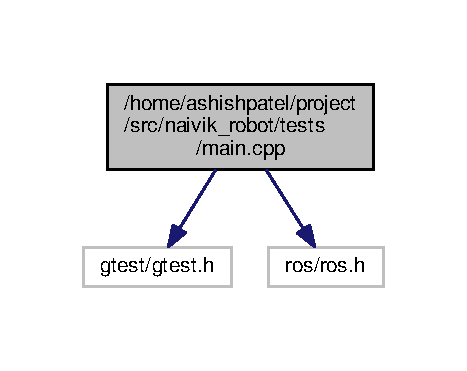
\includegraphics[width=224pt]{main_8cpp__incl}
\end{center}
\end{figure}
\subsection*{Functions}
\begin{DoxyCompactItemize}
\item 
int \hyperlink{main_8cpp_a3c04138a5bfe5d72780bb7e82a18e627}{main} (int argc, char $\ast$$\ast$argv)
\begin{DoxyCompactList}\small\item\em Main function for testing, runs all the tests that were declared with \hyperlink{cameraTest_8cpp_ae703eea73ad1e1cc88652309be0d9be5}{T\+E\+S\+T()} \end{DoxyCompactList}\end{DoxyCompactItemize}


\subsection{Detailed Description}
This file is used to run all the unit tests for the developed package. 

M\+IT License

Copyright (c) 2018 Ashish Patel

Permission is hereby granted, free of charge, to any person obtaining a copy of this software and associated documentation files (the \char`\"{}\+Software\char`\"{}), to deal in the Software without restriction, including without limitation the rights to use, copy, modify, merge, publish, distribute, sublicense, and/or sell copies of the Software, and to permit persons to whom the Software is furnished to do so, subject to the following conditions\+:

The above copyright notice and this permission notice shall be included in all copies or substantial portions of the Software.

T\+HE S\+O\+F\+T\+W\+A\+RE IS P\+R\+O\+V\+I\+D\+ED \char`\"{}\+A\+S I\+S\char`\"{}, W\+I\+T\+H\+O\+UT W\+A\+R\+R\+A\+N\+TY OF A\+NY K\+I\+ND, E\+X\+P\+R\+E\+SS OR I\+M\+P\+L\+I\+ED, I\+N\+C\+L\+U\+D\+I\+NG B\+UT N\+OT L\+I\+M\+I\+T\+ED TO T\+HE W\+A\+R\+R\+A\+N\+T\+I\+ES OF M\+E\+R\+C\+H\+A\+N\+T\+A\+B\+I\+L\+I\+TY, F\+I\+T\+N\+E\+SS F\+OR A P\+A\+R\+T\+I\+C\+U\+L\+AR P\+U\+R\+P\+O\+SE A\+ND N\+O\+N\+I\+N\+F\+R\+I\+N\+G\+E\+M\+E\+NT. IN NO E\+V\+E\+NT S\+H\+A\+LL T\+HE A\+U\+T\+H\+O\+RS OR C\+O\+P\+Y\+R\+I\+G\+HT H\+O\+L\+D\+E\+RS BE L\+I\+A\+B\+LE F\+OR A\+NY C\+L\+A\+IM, D\+A\+M\+A\+G\+ES OR O\+T\+H\+ER L\+I\+A\+B\+I\+L\+I\+TY, W\+H\+E\+T\+H\+ER IN AN A\+C\+T\+I\+ON OF C\+O\+N\+T\+R\+A\+CT, T\+O\+RT OR O\+T\+H\+E\+R\+W\+I\+SE, A\+R\+I\+S\+I\+NG F\+R\+OM, O\+UT OF OR IN C\+O\+N\+N\+E\+C\+T\+I\+ON W\+I\+TH T\+HE S\+O\+F\+T\+W\+A\+RE OR T\+HE U\+SE OR O\+T\+H\+ER D\+E\+A\+L\+I\+N\+GS IN T\+HE S\+O\+F\+T\+W\+A\+RE.

\begin{DoxyVersion}{Version}
0.\+1 
\end{DoxyVersion}
\begin{DoxyAuthor}{Author}
Ashish Patel 
\end{DoxyAuthor}
\begin{DoxyDate}{Date}
12-\/15-\/2018 
\end{DoxyDate}


\subsection{Function Documentation}
\index{main.\+cpp@{main.\+cpp}!main@{main}}
\index{main@{main}!main.\+cpp@{main.\+cpp}}
\subsubsection[{\texorpdfstring{main(int argc, char $\ast$$\ast$argv)}{main(int argc, char **argv)}}]{\setlength{\rightskip}{0pt plus 5cm}int main (
\begin{DoxyParamCaption}
\item[{int}]{argc, }
\item[{char $\ast$$\ast$}]{argv}
\end{DoxyParamCaption}
)}\hypertarget{main_8cpp_a3c04138a5bfe5d72780bb7e82a18e627}{}\label{main_8cpp_a3c04138a5bfe5d72780bb7e82a18e627}


Main function for testing, runs all the tests that were declared with \hyperlink{cameraTest_8cpp_ae703eea73ad1e1cc88652309be0d9be5}{T\+E\+S\+T()} 


\begin{DoxyParams}{Parameters}
{\em argc} & The argc as int \\
\hline
{\em argv} & The argv as char array \\
\hline
\end{DoxyParams}
\begin{DoxyReturn}{Returns}
0, if everything is successful 
\end{DoxyReturn}

\hypertarget{motionControllerTest_8cpp}{}\section{/home/ashishpatel/project/src/naivik\+\_\+robot/tests/motion\+Controller\+Test.cpp File Reference}
\label{motionControllerTest_8cpp}\index{/home/ashishpatel/project/src/naivik\+\_\+robot/tests/motion\+Controller\+Test.\+cpp@{/home/ashishpatel/project/src/naivik\+\_\+robot/tests/motion\+Controller\+Test.\+cpp}}


Test cases for \hyperlink{classMotionController}{Motion\+Controller} class.  


{\ttfamily \#include $<$gtest/gtest.\+h$>$}\\*
{\ttfamily \#include $<$memory$>$}\\*
{\ttfamily \#include \char`\"{}motion\+Controller.\+hpp\char`\"{}}\\*
{\ttfamily \#include \char`\"{}ros/ros.\+h\char`\"{}}\\*
{\ttfamily \#include \char`\"{}geometry\+\_\+msgs/\+Twist.\+h\char`\"{}}\\*
Include dependency graph for motion\+Controller\+Test.\+cpp\+:
\nopagebreak
\begin{figure}[H]
\begin{center}
\leavevmode
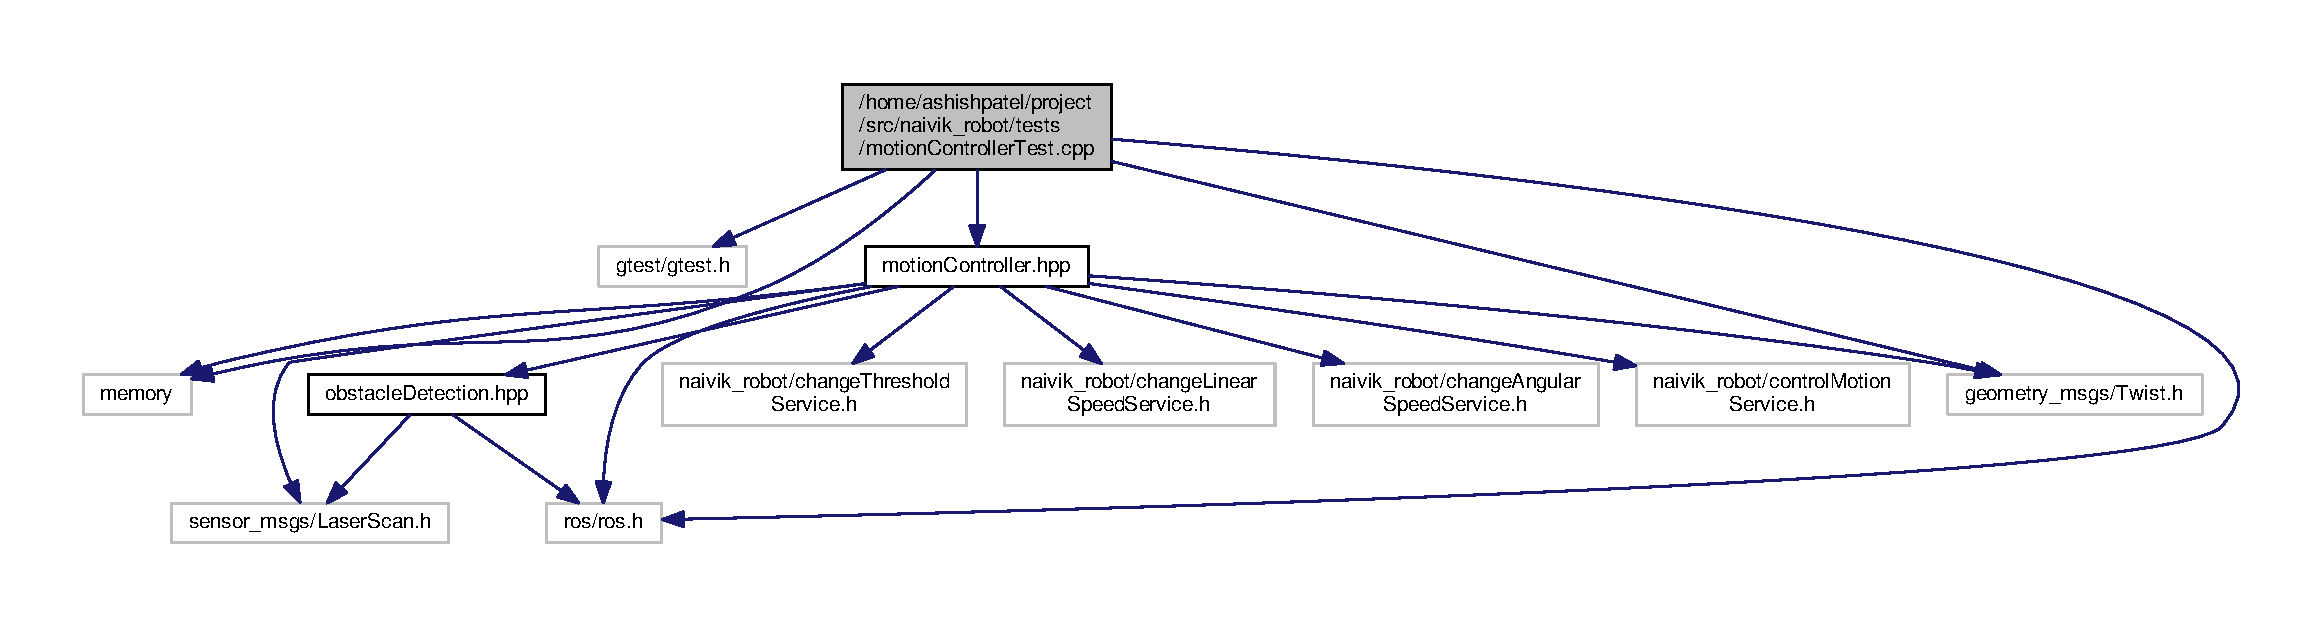
\includegraphics[width=350pt]{motionControllerTest_8cpp__incl}
\end{center}
\end{figure}
\subsection*{Classes}
\begin{DoxyCompactItemize}
\item 
class \hyperlink{classMotionControllerTest}{Motion\+Controller\+Test}
\begin{DoxyCompactList}\small\item\em \hyperlink{classMotionController}{Motion\+Controller} fixture class. \end{DoxyCompactList}\end{DoxyCompactItemize}
\subsection*{Functions}
\begin{DoxyCompactItemize}
\item 
\hyperlink{motionControllerTest_8cpp_ad5f1464be0be316612de51fe95a8b635}{T\+E\+S\+T\+\_\+F} (\hyperlink{classMotionControllerTest}{Motion\+Controller\+Test}, get\+\_\+vehicle\+\_\+action)
\begin{DoxyCompactList}\small\item\em Test the ability to get\+Vehicle\+Action. \end{DoxyCompactList}\item 
\hyperlink{motionControllerTest_8cpp_abdd4e6bbc394134282a4024789f0adaf}{T\+E\+S\+T\+\_\+F} (\hyperlink{classMotionControllerTest}{Motion\+Controller\+Test}, set\+\_\+linear\+\_\+speed)
\begin{DoxyCompactList}\small\item\em Test the ability to get \& set linear\+Speed\+\_\+. \end{DoxyCompactList}\item 
\hyperlink{motionControllerTest_8cpp_a3fe23996bb2c0a2b73cefb588240e9d9}{T\+E\+S\+T\+\_\+F} (\hyperlink{classMotionControllerTest}{Motion\+Controller\+Test}, get\+\_\+linear\+\_\+speed)
\begin{DoxyCompactList}\small\item\em Test the ability to get \& set Angular\+Speed\+\_\+. \end{DoxyCompactList}\end{DoxyCompactItemize}


\subsection{Detailed Description}
Test cases for \hyperlink{classMotionController}{Motion\+Controller} class. 

M\+IT License

Copyright (c) 2018 Ashish Patel

Permission is hereby granted, free of charge, to any person obtaining a copy of this software and associated documentation files (the \char`\"{}\+Software\char`\"{}), to deal in the Software without restriction, including without limitation the rights to use, copy, modify, merge, publish, distribute, sublicense, and/or sell copies of the Software, and to permit persons to whom the Software is furnished to do so, subject to the following conditions\+:

The above copyright notice and this permission notice shall be included in all copies or substantial portions of the Software.

T\+HE S\+O\+F\+T\+W\+A\+RE IS P\+R\+O\+V\+I\+D\+ED \char`\"{}\+A\+S I\+S\char`\"{}, W\+I\+T\+H\+O\+UT W\+A\+R\+R\+A\+N\+TY OF A\+NY K\+I\+ND, E\+X\+P\+R\+E\+SS OR I\+M\+P\+L\+I\+ED, I\+N\+C\+L\+U\+D\+I\+NG B\+UT N\+OT L\+I\+M\+I\+T\+ED TO T\+HE W\+A\+R\+R\+A\+N\+T\+I\+ES OF M\+E\+R\+C\+H\+A\+N\+T\+A\+B\+I\+L\+I\+TY, F\+I\+T\+N\+E\+SS F\+OR A P\+A\+R\+T\+I\+C\+U\+L\+AR P\+U\+R\+P\+O\+SE A\+ND N\+O\+N\+I\+N\+F\+R\+I\+N\+G\+E\+M\+E\+NT. IN NO E\+V\+E\+NT S\+H\+A\+LL T\+HE A\+U\+T\+H\+O\+RS OR C\+O\+P\+Y\+R\+I\+G\+HT H\+O\+L\+D\+E\+RS BE L\+I\+A\+B\+LE F\+OR A\+NY C\+L\+A\+IM, D\+A\+M\+A\+G\+ES OR O\+T\+H\+ER L\+I\+A\+B\+I\+L\+I\+TY, W\+H\+E\+T\+H\+ER IN AN A\+C\+T\+I\+ON OF C\+O\+N\+T\+R\+A\+CT, T\+O\+RT OR O\+T\+H\+E\+R\+W\+I\+SE, A\+R\+I\+S\+I\+NG F\+R\+OM, O\+UT OF OR IN C\+O\+N\+N\+E\+C\+T\+I\+ON W\+I\+TH T\+HE S\+O\+F\+T\+W\+A\+RE OR T\+HE U\+SE OR O\+T\+H\+ER D\+E\+A\+L\+I\+N\+GS IN T\+HE S\+O\+F\+T\+W\+A\+RE.

\begin{DoxyVersion}{Version}
0.\+1 
\end{DoxyVersion}
\begin{DoxyAuthor}{Author}
Ashish Patel 
\end{DoxyAuthor}
\begin{DoxyDate}{Date}
12-\/15-\/2018 
\end{DoxyDate}


\subsection{Function Documentation}
\index{motion\+Controller\+Test.\+cpp@{motion\+Controller\+Test.\+cpp}!T\+E\+S\+T\+\_\+F@{T\+E\+S\+T\+\_\+F}}
\index{T\+E\+S\+T\+\_\+F@{T\+E\+S\+T\+\_\+F}!motion\+Controller\+Test.\+cpp@{motion\+Controller\+Test.\+cpp}}
\subsubsection[{\texorpdfstring{T\+E\+S\+T\+\_\+\+F(\+Motion\+Controller\+Test, get\+\_\+vehicle\+\_\+action)}{TEST_F(MotionControllerTest, get_vehicle_action)}}]{\setlength{\rightskip}{0pt plus 5cm}T\+E\+S\+T\+\_\+F (
\begin{DoxyParamCaption}
\item[{{\bf Motion\+Controller\+Test}}]{, }
\item[{get\+\_\+vehicle\+\_\+action}]{}
\end{DoxyParamCaption}
)}\hypertarget{motionControllerTest_8cpp_ad5f1464be0be316612de51fe95a8b635}{}\label{motionControllerTest_8cpp_ad5f1464be0be316612de51fe95a8b635}


Test the ability to get\+Vehicle\+Action. 

\index{motion\+Controller\+Test.\+cpp@{motion\+Controller\+Test.\+cpp}!T\+E\+S\+T\+\_\+F@{T\+E\+S\+T\+\_\+F}}
\index{T\+E\+S\+T\+\_\+F@{T\+E\+S\+T\+\_\+F}!motion\+Controller\+Test.\+cpp@{motion\+Controller\+Test.\+cpp}}
\subsubsection[{\texorpdfstring{T\+E\+S\+T\+\_\+\+F(\+Motion\+Controller\+Test, set\+\_\+linear\+\_\+speed)}{TEST_F(MotionControllerTest, set_linear_speed)}}]{\setlength{\rightskip}{0pt plus 5cm}T\+E\+S\+T\+\_\+F (
\begin{DoxyParamCaption}
\item[{{\bf Motion\+Controller\+Test}}]{, }
\item[{set\+\_\+linear\+\_\+speed}]{}
\end{DoxyParamCaption}
)}\hypertarget{motionControllerTest_8cpp_abdd4e6bbc394134282a4024789f0adaf}{}\label{motionControllerTest_8cpp_abdd4e6bbc394134282a4024789f0adaf}


Test the ability to get \& set linear\+Speed\+\_\+. 

\index{motion\+Controller\+Test.\+cpp@{motion\+Controller\+Test.\+cpp}!T\+E\+S\+T\+\_\+F@{T\+E\+S\+T\+\_\+F}}
\index{T\+E\+S\+T\+\_\+F@{T\+E\+S\+T\+\_\+F}!motion\+Controller\+Test.\+cpp@{motion\+Controller\+Test.\+cpp}}
\subsubsection[{\texorpdfstring{T\+E\+S\+T\+\_\+\+F(\+Motion\+Controller\+Test, get\+\_\+linear\+\_\+speed)}{TEST_F(MotionControllerTest, get_linear_speed)}}]{\setlength{\rightskip}{0pt plus 5cm}T\+E\+S\+T\+\_\+F (
\begin{DoxyParamCaption}
\item[{{\bf Motion\+Controller\+Test}}]{, }
\item[{get\+\_\+linear\+\_\+speed}]{}
\end{DoxyParamCaption}
)}\hypertarget{motionControllerTest_8cpp_a3fe23996bb2c0a2b73cefb588240e9d9}{}\label{motionControllerTest_8cpp_a3fe23996bb2c0a2b73cefb588240e9d9}


Test the ability to get \& set Angular\+Speed\+\_\+. 


\hypertarget{naivikTest_8cpp}{}\section{/home/ashishpatel/project/src/naivik\+\_\+robot/tests/naivik\+Test.cpp File Reference}
\label{naivikTest_8cpp}\index{/home/ashishpatel/project/src/naivik\+\_\+robot/tests/naivik\+Test.\+cpp@{/home/ashishpatel/project/src/naivik\+\_\+robot/tests/naivik\+Test.\+cpp}}


Test cases for \hyperlink{classNaivik}{Naivik} class.  


{\ttfamily \#include $<$gtest/gtest.\+h$>$}\\*
{\ttfamily \#include \char`\"{}ros/ros.\+h\char`\"{}}\\*
{\ttfamily \#include \char`\"{}naivik.\+hpp\char`\"{}}\\*
Include dependency graph for naivik\+Test.\+cpp\+:
\nopagebreak
\begin{figure}[H]
\begin{center}
\leavevmode
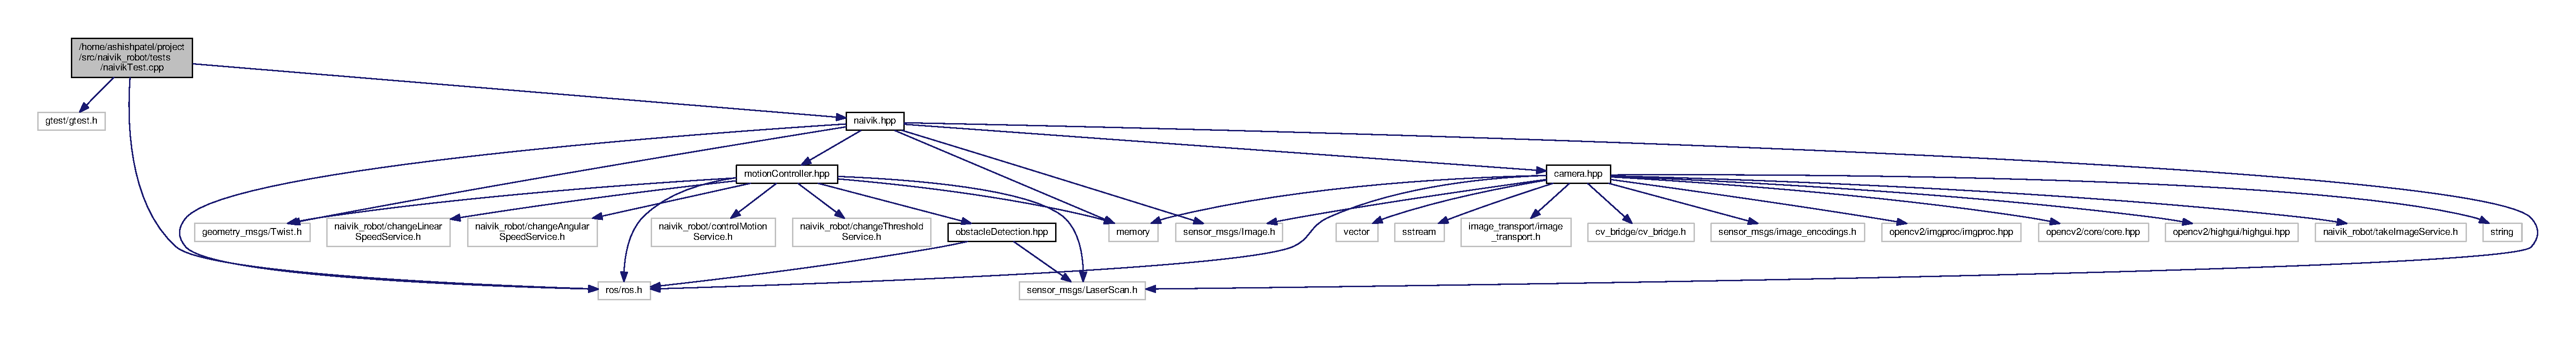
\includegraphics[width=350pt]{naivikTest_8cpp__incl}
\end{center}
\end{figure}
\subsection*{Classes}
\begin{DoxyCompactItemize}
\item 
class \hyperlink{classNaivikTest}{Naivik\+Test}
\begin{DoxyCompactList}\small\item\em \hyperlink{classNaivik}{Naivik} fixture class. \end{DoxyCompactList}\end{DoxyCompactItemize}


\subsection{Detailed Description}
Test cases for \hyperlink{classNaivik}{Naivik} class. 

M\+IT License

Copyright (c) 2018 Ashish Patel

Permission is hereby granted, free of charge, to any person obtaining a copy of this software and associated documentation files (the \char`\"{}\+Software\char`\"{}), to deal in the Software without restriction, including without limitation the rights to use, copy, modify, merge, publish, distribute, sublicense, and/or sell copies of the Software, and to permit persons to whom the Software is furnished to do so, subject to the following conditions\+:

The above copyright notice and this permission notice shall be included in all copies or substantial portions of the Software.

T\+HE S\+O\+F\+T\+W\+A\+RE IS P\+R\+O\+V\+I\+D\+ED \char`\"{}\+A\+S I\+S\char`\"{}, W\+I\+T\+H\+O\+UT W\+A\+R\+R\+A\+N\+TY OF A\+NY K\+I\+ND, E\+X\+P\+R\+E\+SS OR I\+M\+P\+L\+I\+ED, I\+N\+C\+L\+U\+D\+I\+NG B\+UT N\+OT L\+I\+M\+I\+T\+ED TO T\+HE W\+A\+R\+R\+A\+N\+T\+I\+ES OF M\+E\+R\+C\+H\+A\+N\+T\+A\+B\+I\+L\+I\+TY, F\+I\+T\+N\+E\+SS F\+OR A P\+A\+R\+T\+I\+C\+U\+L\+AR P\+U\+R\+P\+O\+SE A\+ND N\+O\+N\+I\+N\+F\+R\+I\+N\+G\+E\+M\+E\+NT. IN NO E\+V\+E\+NT S\+H\+A\+LL T\+HE A\+U\+T\+H\+O\+RS OR C\+O\+P\+Y\+R\+I\+G\+HT H\+O\+L\+D\+E\+RS BE L\+I\+A\+B\+LE F\+OR A\+NY C\+L\+A\+IM, D\+A\+M\+A\+G\+ES OR O\+T\+H\+ER L\+I\+A\+B\+I\+L\+I\+TY, W\+H\+E\+T\+H\+ER IN AN A\+C\+T\+I\+ON OF C\+O\+N\+T\+R\+A\+CT, T\+O\+RT OR O\+T\+H\+E\+R\+W\+I\+SE, A\+R\+I\+S\+I\+NG F\+R\+OM, O\+UT OF OR IN C\+O\+N\+N\+E\+C\+T\+I\+ON W\+I\+TH T\+HE S\+O\+F\+T\+W\+A\+RE OR T\+HE U\+SE OR O\+T\+H\+ER D\+E\+A\+L\+I\+N\+GS IN T\+HE S\+O\+F\+T\+W\+A\+RE.

\begin{DoxyVersion}{Version}
0.\+1 
\end{DoxyVersion}
\begin{DoxyAuthor}{Author}
Ashish Patel 
\end{DoxyAuthor}
\begin{DoxyDate}{Date}
12-\/15-\/2018 
\end{DoxyDate}

\hypertarget{obstacleDetectionTest_8cpp}{}\section{/home/ashishpatel/project/src/naivik\+\_\+robot/tests/obstacle\+Detection\+Test.cpp File Reference}
\label{obstacleDetectionTest_8cpp}\index{/home/ashishpatel/project/src/naivik\+\_\+robot/tests/obstacle\+Detection\+Test.\+cpp@{/home/ashishpatel/project/src/naivik\+\_\+robot/tests/obstacle\+Detection\+Test.\+cpp}}


Test cases for \hyperlink{classObstacleDetection}{Obstacle\+Detection} class.  


{\ttfamily \#include $<$gtest/gtest.\+h$>$}\\*
{\ttfamily \#include $<$memory$>$}\\*
{\ttfamily \#include \char`\"{}obstacle\+Detection.\+hpp\char`\"{}}\\*
{\ttfamily \#include \char`\"{}ros/ros.\+h\char`\"{}}\\*
Include dependency graph for obstacle\+Detection\+Test.\+cpp\+:
\nopagebreak
\begin{figure}[H]
\begin{center}
\leavevmode
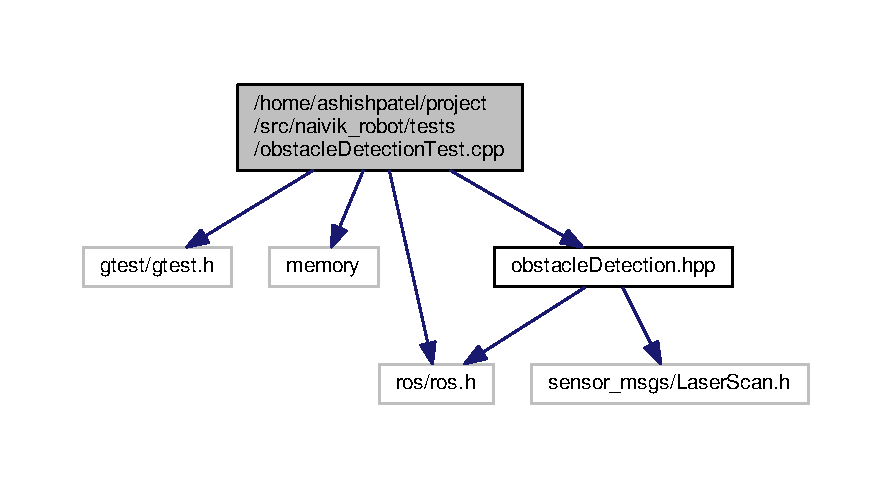
\includegraphics[width=350pt]{obstacleDetectionTest_8cpp__incl}
\end{center}
\end{figure}
\subsection*{Classes}
\begin{DoxyCompactItemize}
\item 
class \hyperlink{classObstacleDetectionTest}{Obstacle\+Detection\+Test}
\begin{DoxyCompactList}\small\item\em \hyperlink{classObstacleDetection}{Obstacle\+Detection} fixture class. \end{DoxyCompactList}\end{DoxyCompactItemize}
\subsection*{Functions}
\begin{DoxyCompactItemize}
\item 
\hyperlink{obstacleDetectionTest_8cpp_a52b97b5647f2972745fa668592745a05}{T\+E\+S\+T\+\_\+F} (\hyperlink{classObstacleDetectionTest}{Obstacle\+Detection\+Test}, get\+\_\+distance\+\_\+threshold)
\begin{DoxyCompactList}\small\item\em Test the ability to get dist\+Threshold\+\_\+ variable. \end{DoxyCompactList}\item 
\hyperlink{obstacleDetectionTest_8cpp_a01b327fc6aa16f94e34493ea365dda7b}{T\+E\+S\+T\+\_\+F} (\hyperlink{classObstacleDetectionTest}{Obstacle\+Detection\+Test}, set\+\_\+distance\+\_\+threshold)
\begin{DoxyCompactList}\small\item\em Test the ability to set dist\+Threshold\+\_\+ variable. \end{DoxyCompactList}\end{DoxyCompactItemize}


\subsection{Detailed Description}
Test cases for \hyperlink{classObstacleDetection}{Obstacle\+Detection} class. 

M\+IT License

Copyright (c) 2018 Ashish Patel

Permission is hereby granted, free of charge, to any person obtaining a copy of this software and associated documentation files (the \char`\"{}\+Software\char`\"{}), to deal in the Software without restriction, including without limitation the rights to use, copy, modify, merge, publish, distribute, sublicense, and/or sell copies of the Software, and to permit persons to whom the Software is furnished to do so, subject to the following conditions\+:

The above copyright notice and this permission notice shall be included in all copies or substantial portions of the Software.

T\+HE S\+O\+F\+T\+W\+A\+RE IS P\+R\+O\+V\+I\+D\+ED \char`\"{}\+A\+S I\+S\char`\"{}, W\+I\+T\+H\+O\+UT W\+A\+R\+R\+A\+N\+TY OF A\+NY K\+I\+ND, E\+X\+P\+R\+E\+SS OR I\+M\+P\+L\+I\+ED, I\+N\+C\+L\+U\+D\+I\+NG B\+UT N\+OT L\+I\+M\+I\+T\+ED TO T\+HE W\+A\+R\+R\+A\+N\+T\+I\+ES OF M\+E\+R\+C\+H\+A\+N\+T\+A\+B\+I\+L\+I\+TY, F\+I\+T\+N\+E\+SS F\+OR A P\+A\+R\+T\+I\+C\+U\+L\+AR P\+U\+R\+P\+O\+SE A\+ND N\+O\+N\+I\+N\+F\+R\+I\+N\+G\+E\+M\+E\+NT. IN NO E\+V\+E\+NT S\+H\+A\+LL T\+HE A\+U\+T\+H\+O\+RS OR C\+O\+P\+Y\+R\+I\+G\+HT H\+O\+L\+D\+E\+RS BE L\+I\+A\+B\+LE F\+OR A\+NY C\+L\+A\+IM, D\+A\+M\+A\+G\+ES OR O\+T\+H\+ER L\+I\+A\+B\+I\+L\+I\+TY, W\+H\+E\+T\+H\+ER IN AN A\+C\+T\+I\+ON OF C\+O\+N\+T\+R\+A\+CT, T\+O\+RT OR O\+T\+H\+E\+R\+W\+I\+SE, A\+R\+I\+S\+I\+NG F\+R\+OM, O\+UT OF OR IN C\+O\+N\+N\+E\+C\+T\+I\+ON W\+I\+TH T\+HE S\+O\+F\+T\+W\+A\+RE OR T\+HE U\+SE OR O\+T\+H\+ER D\+E\+A\+L\+I\+N\+GS IN T\+HE S\+O\+F\+T\+W\+A\+RE.

\begin{DoxyVersion}{Version}
0.\+1 
\end{DoxyVersion}
\begin{DoxyAuthor}{Author}
Ashish Patel 
\end{DoxyAuthor}
\begin{DoxyDate}{Date}
12-\/15-\/2018 
\end{DoxyDate}


\subsection{Function Documentation}
\index{obstacle\+Detection\+Test.\+cpp@{obstacle\+Detection\+Test.\+cpp}!T\+E\+S\+T\+\_\+F@{T\+E\+S\+T\+\_\+F}}
\index{T\+E\+S\+T\+\_\+F@{T\+E\+S\+T\+\_\+F}!obstacle\+Detection\+Test.\+cpp@{obstacle\+Detection\+Test.\+cpp}}
\subsubsection[{\texorpdfstring{T\+E\+S\+T\+\_\+\+F(\+Obstacle\+Detection\+Test, get\+\_\+distance\+\_\+threshold)}{TEST_F(ObstacleDetectionTest, get_distance_threshold)}}]{\setlength{\rightskip}{0pt plus 5cm}T\+E\+S\+T\+\_\+F (
\begin{DoxyParamCaption}
\item[{{\bf Obstacle\+Detection\+Test}}]{, }
\item[{get\+\_\+distance\+\_\+threshold}]{}
\end{DoxyParamCaption}
)}\hypertarget{obstacleDetectionTest_8cpp_a52b97b5647f2972745fa668592745a05}{}\label{obstacleDetectionTest_8cpp_a52b97b5647f2972745fa668592745a05}


Test the ability to get dist\+Threshold\+\_\+ variable. 

\index{obstacle\+Detection\+Test.\+cpp@{obstacle\+Detection\+Test.\+cpp}!T\+E\+S\+T\+\_\+F@{T\+E\+S\+T\+\_\+F}}
\index{T\+E\+S\+T\+\_\+F@{T\+E\+S\+T\+\_\+F}!obstacle\+Detection\+Test.\+cpp@{obstacle\+Detection\+Test.\+cpp}}
\subsubsection[{\texorpdfstring{T\+E\+S\+T\+\_\+\+F(\+Obstacle\+Detection\+Test, set\+\_\+distance\+\_\+threshold)}{TEST_F(ObstacleDetectionTest, set_distance_threshold)}}]{\setlength{\rightskip}{0pt plus 5cm}T\+E\+S\+T\+\_\+F (
\begin{DoxyParamCaption}
\item[{{\bf Obstacle\+Detection\+Test}}]{, }
\item[{set\+\_\+distance\+\_\+threshold}]{}
\end{DoxyParamCaption}
)}\hypertarget{obstacleDetectionTest_8cpp_a01b327fc6aa16f94e34493ea365dda7b}{}\label{obstacleDetectionTest_8cpp_a01b327fc6aa16f94e34493ea365dda7b}


Test the ability to set dist\+Threshold\+\_\+ variable. 


\hypertarget{testHelper_8cpp}{}\section{/home/ashishpatel/project/src/naivik\+\_\+robot/tests/test\+Helper.cpp File Reference}
\label{testHelper_8cpp}\index{/home/ashishpatel/project/src/naivik\+\_\+robot/tests/test\+Helper.\+cpp@{/home/ashishpatel/project/src/naivik\+\_\+robot/tests/test\+Helper.\+cpp}}


\hyperlink{classTestHelper}{Test\+Helper} implementation file.  


{\ttfamily \#include \char`\"{}ros/ros.\+h\char`\"{}}\\*
{\ttfamily \#include \char`\"{}geometry\+\_\+msgs/\+Twist.\+h\char`\"{}}\\*
{\ttfamily \#include \char`\"{}test\+Helper.\+hpp\char`\"{}}\\*
Include dependency graph for test\+Helper.\+cpp\+:
\nopagebreak
\begin{figure}[H]
\begin{center}
\leavevmode
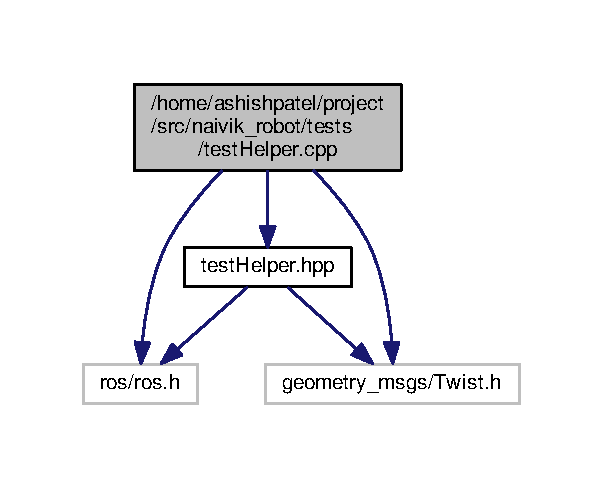
\includegraphics[width=290pt]{testHelper_8cpp__incl}
\end{center}
\end{figure}


\subsection{Detailed Description}
\hyperlink{classTestHelper}{Test\+Helper} implementation file. 

M\+IT License

Copyright (c) 2018 Ashish Patel

Permission is hereby granted, free of charge, to any person obtaining a copy of this software and associated documentation files (the \char`\"{}\+Software\char`\"{}), to deal in the Software without restriction, including without limitation the rights to use, copy, modify, merge, publish, distribute, sublicense, and/or sell copies of the Software, and to permit persons to whom the Software is furnished to do so, subject to the following conditions\+:

The above copyright notice and this permission notice shall be included in all copies or substantial portions of the Software.

T\+HE S\+O\+F\+T\+W\+A\+RE IS P\+R\+O\+V\+I\+D\+ED \char`\"{}\+A\+S I\+S\char`\"{}, W\+I\+T\+H\+O\+UT W\+A\+R\+R\+A\+N\+TY OF A\+NY K\+I\+ND, E\+X\+P\+R\+E\+SS OR I\+M\+P\+L\+I\+ED, I\+N\+C\+L\+U\+D\+I\+NG B\+UT N\+OT L\+I\+M\+I\+T\+ED TO T\+HE W\+A\+R\+R\+A\+N\+T\+I\+ES OF M\+E\+R\+C\+H\+A\+N\+T\+A\+B\+I\+L\+I\+TY, F\+I\+T\+N\+E\+SS F\+OR A P\+A\+R\+T\+I\+C\+U\+L\+AR P\+U\+R\+P\+O\+SE A\+ND N\+O\+N\+I\+N\+F\+R\+I\+N\+G\+E\+M\+E\+NT. IN NO E\+V\+E\+NT S\+H\+A\+LL T\+HE A\+U\+T\+H\+O\+RS OR C\+O\+P\+Y\+R\+I\+G\+HT H\+O\+L\+D\+E\+RS BE L\+I\+A\+B\+LE F\+OR A\+NY C\+L\+A\+IM, D\+A\+M\+A\+G\+ES OR O\+T\+H\+ER L\+I\+A\+B\+I\+L\+I\+TY, W\+H\+E\+T\+H\+ER IN AN A\+C\+T\+I\+ON OF C\+O\+N\+T\+R\+A\+CT, T\+O\+RT OR O\+T\+H\+E\+R\+W\+I\+SE, A\+R\+I\+S\+I\+NG F\+R\+OM, O\+UT OF OR IN C\+O\+N\+N\+E\+C\+T\+I\+ON W\+I\+TH T\+HE S\+O\+F\+T\+W\+A\+RE OR T\+HE U\+SE OR O\+T\+H\+ER D\+E\+A\+L\+I\+N\+GS IN T\+HE S\+O\+F\+T\+W\+A\+RE.

\begin{DoxyVersion}{Version}
0.\+1 
\end{DoxyVersion}
\begin{DoxyAuthor}{Author}
Ashish Patel 
\end{DoxyAuthor}
\begin{DoxyDate}{Date}
12-\/15-\/2018 
\end{DoxyDate}

\hypertarget{testHelper_8hpp}{}\section{/home/ashishpatel/project/src/naivik\+\_\+robot/tests/test\+Helper.hpp File Reference}
\label{testHelper_8hpp}\index{/home/ashishpatel/project/src/naivik\+\_\+robot/tests/test\+Helper.\+hpp@{/home/ashishpatel/project/src/naivik\+\_\+robot/tests/test\+Helper.\+hpp}}


Header file for \hyperlink{classTestHelper}{Test\+Helper} class.  


{\ttfamily \#include \char`\"{}ros/ros.\+h\char`\"{}}\\*
{\ttfamily \#include \char`\"{}geometry\+\_\+msgs/\+Twist.\+h\char`\"{}}\\*
Include dependency graph for test\+Helper.\+hpp\+:
\nopagebreak
\begin{figure}[H]
\begin{center}
\leavevmode
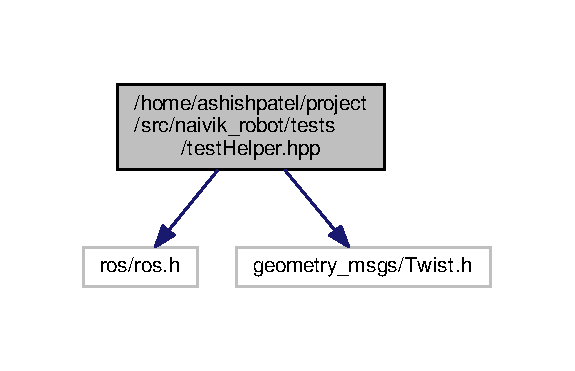
\includegraphics[width=276pt]{testHelper_8hpp__incl}
\end{center}
\end{figure}
This graph shows which files directly or indirectly include this file\+:
\nopagebreak
\begin{figure}[H]
\begin{center}
\leavevmode
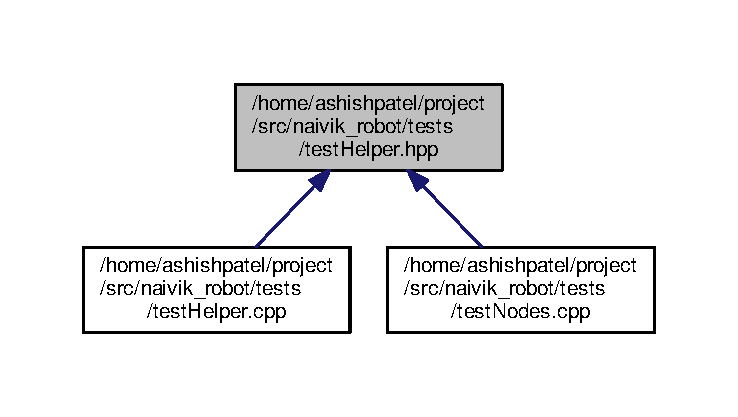
\includegraphics[width=350pt]{testHelper_8hpp__dep__incl}
\end{center}
\end{figure}
\subsection*{Classes}
\begin{DoxyCompactItemize}
\item 
class \hyperlink{classTestHelper}{Test\+Helper}
\begin{DoxyCompactList}\small\item\em \hyperlink{classTestHelper}{Test\+Helper} class handles in testing the nodes publisher and subscriber. \end{DoxyCompactList}\end{DoxyCompactItemize}


\subsection{Detailed Description}
Header file for \hyperlink{classTestHelper}{Test\+Helper} class. 

M\+IT License

Copyright (c) 2018 Ashish Patel

Permission is hereby granted, free of charge, to any person obtaining a copy of this software and associated documentation files (the \char`\"{}\+Software\char`\"{}), to deal in the Software without restriction, including without limitation the rights to use, copy, modify, merge, publish, distribute, sublicense, and/or sell copies of the Software, and to permit persons to whom the Software is furnished to do so, subject to the following conditions\+:

The above copyright notice and this permission notice shall be included in all copies or substantial portions of the Software.

T\+HE S\+O\+F\+T\+W\+A\+RE IS P\+R\+O\+V\+I\+D\+ED \char`\"{}\+A\+S I\+S\char`\"{}, W\+I\+T\+H\+O\+UT W\+A\+R\+R\+A\+N\+TY OF A\+NY K\+I\+ND, E\+X\+P\+R\+E\+SS OR I\+M\+P\+L\+I\+ED, I\+N\+C\+L\+U\+D\+I\+NG B\+UT N\+OT L\+I\+M\+I\+T\+ED TO T\+HE W\+A\+R\+R\+A\+N\+T\+I\+ES OF M\+E\+R\+C\+H\+A\+N\+T\+A\+B\+I\+L\+I\+TY, F\+I\+T\+N\+E\+SS F\+OR A P\+A\+R\+T\+I\+C\+U\+L\+AR P\+U\+R\+P\+O\+SE A\+ND N\+O\+N\+I\+N\+F\+R\+I\+N\+G\+E\+M\+E\+NT. IN NO E\+V\+E\+NT S\+H\+A\+LL T\+HE A\+U\+T\+H\+O\+RS OR C\+O\+P\+Y\+R\+I\+G\+HT H\+O\+L\+D\+E\+RS BE L\+I\+A\+B\+LE F\+OR A\+NY C\+L\+A\+IM, D\+A\+M\+A\+G\+ES OR O\+T\+H\+ER L\+I\+A\+B\+I\+L\+I\+TY, W\+H\+E\+T\+H\+ER IN AN A\+C\+T\+I\+ON OF C\+O\+N\+T\+R\+A\+CT, T\+O\+RT OR O\+T\+H\+E\+R\+W\+I\+SE, A\+R\+I\+S\+I\+NG F\+R\+OM, O\+UT OF OR IN C\+O\+N\+N\+E\+C\+T\+I\+ON W\+I\+TH T\+HE S\+O\+F\+T\+W\+A\+RE OR T\+HE U\+SE OR O\+T\+H\+ER D\+E\+A\+L\+I\+N\+GS IN T\+HE S\+O\+F\+T\+W\+A\+RE.

\begin{DoxyVersion}{Version}
0.\+1 
\end{DoxyVersion}
\begin{DoxyAuthor}{Author}
Ashish Patel 
\end{DoxyAuthor}
\begin{DoxyDate}{Date}
12-\/15-\/2018 
\end{DoxyDate}

\hypertarget{testNodes_8cpp}{}\section{/home/ashishpatel/project/src/naivik\+\_\+robot/tests/test\+Nodes.cpp File Reference}
\label{testNodes_8cpp}\index{/home/ashishpatel/project/src/naivik\+\_\+robot/tests/test\+Nodes.\+cpp@{/home/ashishpatel/project/src/naivik\+\_\+robot/tests/test\+Nodes.\+cpp}}
{\ttfamily \#include $<$gtest/gtest.\+h$>$}\\*
{\ttfamily \#include \char`\"{}ros/ros.\+h\char`\"{}}\\*
{\ttfamily \#include \char`\"{}sensor\+\_\+msgs/\+Laser\+Scan.\+h\char`\"{}}\\*
{\ttfamily \#include \char`\"{}geometry\+\_\+msgs/\+Twist.\+h\char`\"{}}\\*
{\ttfamily \#include \char`\"{}sensor\+\_\+msgs/\+Image.\+h\char`\"{}}\\*
{\ttfamily \#include \char`\"{}naivik.\+hpp\char`\"{}}\\*
{\ttfamily \#include \char`\"{}motion\+Controller.\+hpp\char`\"{}}\\*
{\ttfamily \#include \char`\"{}camera.\+hpp\char`\"{}}\\*
{\ttfamily \#include \char`\"{}test\+Helper.\+hpp\char`\"{}}\\*
Include dependency graph for test\+Nodes.\+cpp\+:
\nopagebreak
\begin{figure}[H]
\begin{center}
\leavevmode
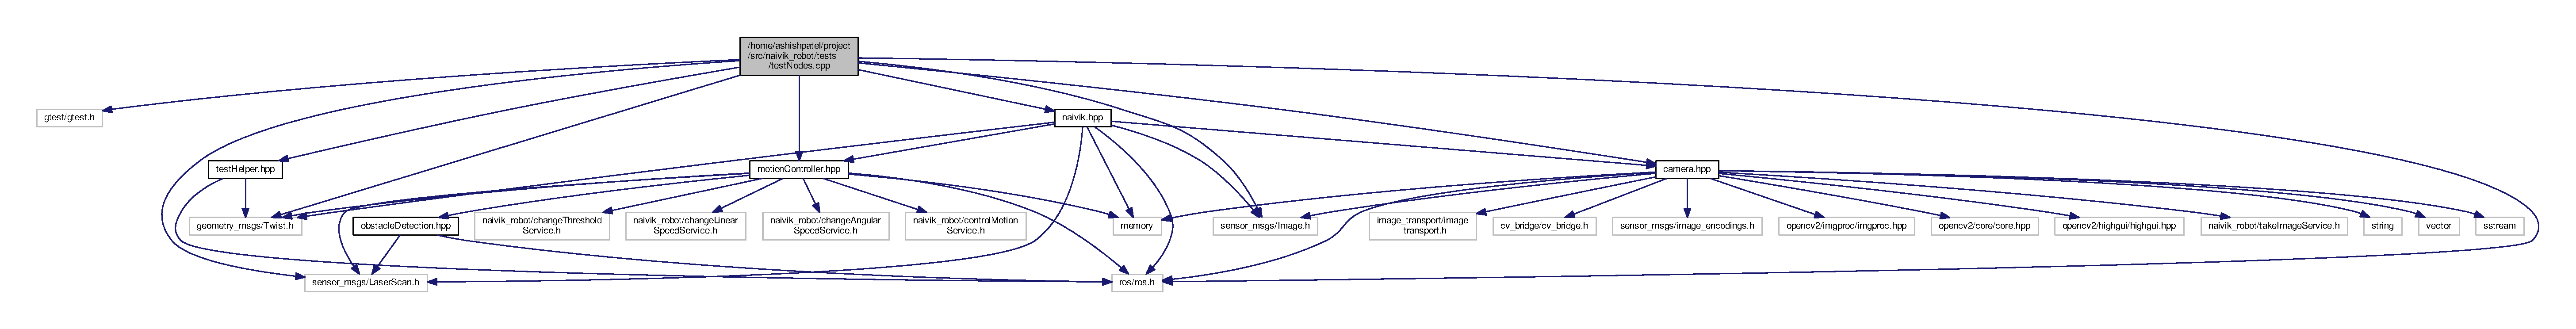
\includegraphics[width=350pt]{testNodes_8cpp__incl}
\end{center}
\end{figure}
\subsection*{Functions}
\begin{DoxyCompactItemize}
\item 
\hyperlink{testNodes_8cpp_a058607d33b6d2afc869f4a8e1568e7bd}{T\+E\+ST} (Testing\+Callbacks, camera\+\_\+callback\+\_\+init)
\begin{DoxyCompactList}\small\item\em To test whether the camera subscriber is initialize properly or not. \end{DoxyCompactList}\item 
\hyperlink{testNodes_8cpp_a53725141d36b27b51d904965799f6812}{T\+E\+ST} (Testing\+Callbacks, laser\+\_\+callback\+\_\+init)
\begin{DoxyCompactList}\small\item\em To test whether the laser subscriber is initialize properly or not. \end{DoxyCompactList}\item 
\hyperlink{testNodes_8cpp_a0bc1c9432e3f9621baeffbb8f5c4f523}{T\+E\+ST} (Testing\+Callbacks, velocity\+\_\+callback\+\_\+init)
\begin{DoxyCompactList}\small\item\em To test whether the velocity publisher is initialize properly or not. \end{DoxyCompactList}\item 
\hyperlink{testNodes_8cpp_a4b037584d549e7466798247eaf491ef2}{T\+E\+ST} (Testing\+Callbacks, non\+\_\+obstacle\+\_\+collision)
\begin{DoxyCompactList}\small\item\em To test determine action function of \hyperlink{classMotionController}{Motion\+Controller} class in a situation when there is no obstacle. \end{DoxyCompactList}\item 
\hyperlink{testNodes_8cpp_a207ec5fad15186507ec9ac47a930b596}{T\+E\+ST} (Testing\+Callbacks, obstacle\+\_\+collision)
\begin{DoxyCompactList}\small\item\em To test determine action function of \hyperlink{classMotionController}{Motion\+Controller} class in a situation when there is an obstacle. \end{DoxyCompactList}\item 
\hyperlink{testNodes_8cpp_a618b5c5bf252cec611bfa07fbcab41cb}{T\+E\+ST} (Testing\+Callbacks, camera\+\_\+callback)
\begin{DoxyCompactList}\small\item\em To test whether the camera callback function. \end{DoxyCompactList}\item 
int \hyperlink{testNodes_8cpp_a3c04138a5bfe5d72780bb7e82a18e627}{main} (int argc, char $\ast$$\ast$argv)
\begin{DoxyCompactList}\small\item\em Main function for testing, runs all the tests that were declared with \hyperlink{testNodes_8cpp_a058607d33b6d2afc869f4a8e1568e7bd}{T\+E\+S\+T()} \end{DoxyCompactList}\end{DoxyCompactItemize}


\subsection{Function Documentation}
\index{test\+Nodes.\+cpp@{test\+Nodes.\+cpp}!main@{main}}
\index{main@{main}!test\+Nodes.\+cpp@{test\+Nodes.\+cpp}}
\subsubsection[{\texorpdfstring{main(int argc, char $\ast$$\ast$argv)}{main(int argc, char **argv)}}]{\setlength{\rightskip}{0pt plus 5cm}int main (
\begin{DoxyParamCaption}
\item[{int}]{argc, }
\item[{char $\ast$$\ast$}]{argv}
\end{DoxyParamCaption}
)}\hypertarget{testNodes_8cpp_a3c04138a5bfe5d72780bb7e82a18e627}{}\label{testNodes_8cpp_a3c04138a5bfe5d72780bb7e82a18e627}


Main function for testing, runs all the tests that were declared with \hyperlink{testNodes_8cpp_a058607d33b6d2afc869f4a8e1568e7bd}{T\+E\+S\+T()} 


\begin{DoxyParams}{Parameters}
{\em argc} & The argc as int \\
\hline
{\em argv} & The argv as char array \\
\hline
\end{DoxyParams}
\begin{DoxyReturn}{Returns}
0, if everything is successful 
\end{DoxyReturn}
\index{test\+Nodes.\+cpp@{test\+Nodes.\+cpp}!T\+E\+ST@{T\+E\+ST}}
\index{T\+E\+ST@{T\+E\+ST}!test\+Nodes.\+cpp@{test\+Nodes.\+cpp}}
\subsubsection[{\texorpdfstring{T\+E\+S\+T(\+Testing\+Callbacks, camera\+\_\+callback\+\_\+init)}{TEST(TestingCallbacks, camera_callback_init)}}]{\setlength{\rightskip}{0pt plus 5cm}T\+E\+ST (
\begin{DoxyParamCaption}
\item[{Testing\+Callbacks}]{, }
\item[{camera\+\_\+callback\+\_\+init}]{}
\end{DoxyParamCaption}
)}\hypertarget{testNodes_8cpp_a058607d33b6d2afc869f4a8e1568e7bd}{}\label{testNodes_8cpp_a058607d33b6d2afc869f4a8e1568e7bd}


To test whether the camera subscriber is initialize properly or not. 

\index{test\+Nodes.\+cpp@{test\+Nodes.\+cpp}!T\+E\+ST@{T\+E\+ST}}
\index{T\+E\+ST@{T\+E\+ST}!test\+Nodes.\+cpp@{test\+Nodes.\+cpp}}
\subsubsection[{\texorpdfstring{T\+E\+S\+T(\+Testing\+Callbacks, laser\+\_\+callback\+\_\+init)}{TEST(TestingCallbacks, laser_callback_init)}}]{\setlength{\rightskip}{0pt plus 5cm}T\+E\+ST (
\begin{DoxyParamCaption}
\item[{Testing\+Callbacks}]{, }
\item[{laser\+\_\+callback\+\_\+init}]{}
\end{DoxyParamCaption}
)}\hypertarget{testNodes_8cpp_a53725141d36b27b51d904965799f6812}{}\label{testNodes_8cpp_a53725141d36b27b51d904965799f6812}


To test whether the laser subscriber is initialize properly or not. 

\index{test\+Nodes.\+cpp@{test\+Nodes.\+cpp}!T\+E\+ST@{T\+E\+ST}}
\index{T\+E\+ST@{T\+E\+ST}!test\+Nodes.\+cpp@{test\+Nodes.\+cpp}}
\subsubsection[{\texorpdfstring{T\+E\+S\+T(\+Testing\+Callbacks, velocity\+\_\+callback\+\_\+init)}{TEST(TestingCallbacks, velocity_callback_init)}}]{\setlength{\rightskip}{0pt plus 5cm}T\+E\+ST (
\begin{DoxyParamCaption}
\item[{Testing\+Callbacks}]{, }
\item[{velocity\+\_\+callback\+\_\+init}]{}
\end{DoxyParamCaption}
)}\hypertarget{testNodes_8cpp_a0bc1c9432e3f9621baeffbb8f5c4f523}{}\label{testNodes_8cpp_a0bc1c9432e3f9621baeffbb8f5c4f523}


To test whether the velocity publisher is initialize properly or not. 

\index{test\+Nodes.\+cpp@{test\+Nodes.\+cpp}!T\+E\+ST@{T\+E\+ST}}
\index{T\+E\+ST@{T\+E\+ST}!test\+Nodes.\+cpp@{test\+Nodes.\+cpp}}
\subsubsection[{\texorpdfstring{T\+E\+S\+T(\+Testing\+Callbacks, non\+\_\+obstacle\+\_\+collision)}{TEST(TestingCallbacks, non_obstacle_collision)}}]{\setlength{\rightskip}{0pt plus 5cm}T\+E\+ST (
\begin{DoxyParamCaption}
\item[{Testing\+Callbacks}]{, }
\item[{non\+\_\+obstacle\+\_\+collision}]{}
\end{DoxyParamCaption}
)}\hypertarget{testNodes_8cpp_a4b037584d549e7466798247eaf491ef2}{}\label{testNodes_8cpp_a4b037584d549e7466798247eaf491ef2}


To test determine action function of \hyperlink{classMotionController}{Motion\+Controller} class in a situation when there is no obstacle. 

\index{test\+Nodes.\+cpp@{test\+Nodes.\+cpp}!T\+E\+ST@{T\+E\+ST}}
\index{T\+E\+ST@{T\+E\+ST}!test\+Nodes.\+cpp@{test\+Nodes.\+cpp}}
\subsubsection[{\texorpdfstring{T\+E\+S\+T(\+Testing\+Callbacks, obstacle\+\_\+collision)}{TEST(TestingCallbacks, obstacle_collision)}}]{\setlength{\rightskip}{0pt plus 5cm}T\+E\+ST (
\begin{DoxyParamCaption}
\item[{Testing\+Callbacks}]{, }
\item[{obstacle\+\_\+collision}]{}
\end{DoxyParamCaption}
)}\hypertarget{testNodes_8cpp_a207ec5fad15186507ec9ac47a930b596}{}\label{testNodes_8cpp_a207ec5fad15186507ec9ac47a930b596}


To test determine action function of \hyperlink{classMotionController}{Motion\+Controller} class in a situation when there is an obstacle. 

\index{test\+Nodes.\+cpp@{test\+Nodes.\+cpp}!T\+E\+ST@{T\+E\+ST}}
\index{T\+E\+ST@{T\+E\+ST}!test\+Nodes.\+cpp@{test\+Nodes.\+cpp}}
\subsubsection[{\texorpdfstring{T\+E\+S\+T(\+Testing\+Callbacks, camera\+\_\+callback)}{TEST(TestingCallbacks, camera_callback)}}]{\setlength{\rightskip}{0pt plus 5cm}T\+E\+ST (
\begin{DoxyParamCaption}
\item[{Testing\+Callbacks}]{, }
\item[{camera\+\_\+callback}]{}
\end{DoxyParamCaption}
)}\hypertarget{testNodes_8cpp_a618b5c5bf252cec611bfa07fbcab41cb}{}\label{testNodes_8cpp_a618b5c5bf252cec611bfa07fbcab41cb}


To test whether the camera callback function. 


\hypertarget{testService_8cpp}{}\section{/home/ashishpatel/project/src/naivik\+\_\+robot/tests/test\+Service.cpp File Reference}
\label{testService_8cpp}\index{/home/ashishpatel/project/src/naivik\+\_\+robot/tests/test\+Service.\+cpp@{/home/ashishpatel/project/src/naivik\+\_\+robot/tests/test\+Service.\+cpp}}


This file is used to test R\+OS Services created.  


{\ttfamily \#include $<$gtest/gtest.\+h$>$}\\*
{\ttfamily \#include \char`\"{}ros/ros.\+h\char`\"{}}\\*
{\ttfamily \#include \char`\"{}ros/service\+\_\+client.\+h\char`\"{}}\\*
{\ttfamily \#include \char`\"{}sensor\+\_\+msgs/\+Laser\+Scan.\+h\char`\"{}}\\*
{\ttfamily \#include \char`\"{}sensor\+\_\+msgs/image\+\_\+encodings.\+h\char`\"{}}\\*
{\ttfamily \#include \char`\"{}naivik.\+hpp\char`\"{}}\\*
{\ttfamily \#include \char`\"{}motion\+Controller.\+hpp\char`\"{}}\\*
{\ttfamily \#include \char`\"{}camera.\+hpp\char`\"{}}\\*
{\ttfamily \#include \char`\"{}naivik\+\_\+robot/change\+Threshold\+Service.\+h\char`\"{}}\\*
{\ttfamily \#include \char`\"{}naivik\+\_\+robot/change\+Linear\+Speed\+Service.\+h\char`\"{}}\\*
{\ttfamily \#include \char`\"{}naivik\+\_\+robot/change\+Angular\+Speed\+Service.\+h\char`\"{}}\\*
{\ttfamily \#include \char`\"{}naivik\+\_\+robot/control\+Motion\+Service.\+h\char`\"{}}\\*
{\ttfamily \#include \char`\"{}naivik\+\_\+robot/take\+Image\+Service.\+h\char`\"{}}\\*
Include dependency graph for test\+Service.\+cpp\+:
\nopagebreak
\begin{figure}[H]
\begin{center}
\leavevmode
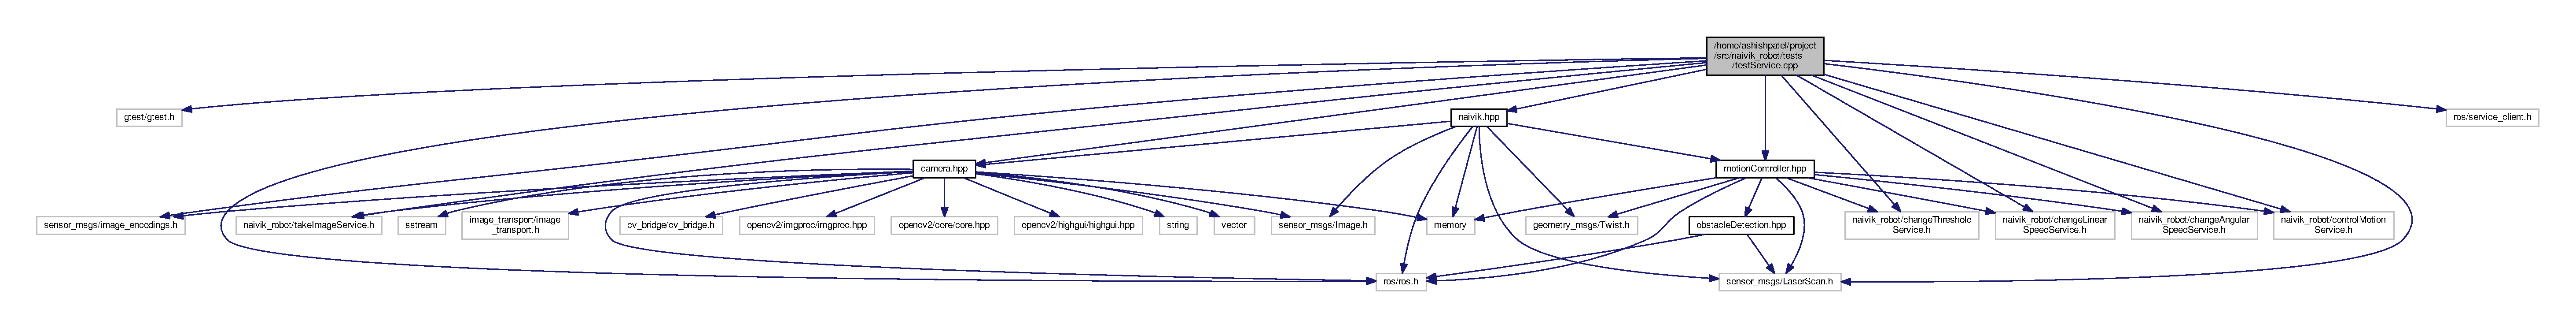
\includegraphics[width=350pt]{testService_8cpp__incl}
\end{center}
\end{figure}
\subsection*{Functions}
\begin{DoxyCompactItemize}
\item 
\hyperlink{testService_8cpp_a647fc12350202341e5b5d643f1188e84}{T\+E\+ST} (test\+\_\+\+Services, change\+\_\+threshold\+\_\+service)
\begin{DoxyCompactList}\small\item\em Testing the change\+Threshold\+Service. \end{DoxyCompactList}\item 
\hyperlink{testService_8cpp_ac060a053eba71d8165a8bbbaf01f4a5e}{T\+E\+ST} (test\+\_\+\+Services, change\+\_\+linear\+\_\+speed\+\_\+service)
\begin{DoxyCompactList}\small\item\em Testing the change\+Linear\+Speed\+Service. \end{DoxyCompactList}\item 
\hyperlink{testService_8cpp_a704ed3477bb685c8d35755327d8e8ded}{T\+E\+ST} (test\+\_\+\+Services, change\+\_\+angular\+\_\+speed\+\_\+service)
\begin{DoxyCompactList}\small\item\em Testing the change\+Angular\+Speed\+Service. \end{DoxyCompactList}\item 
\hyperlink{testService_8cpp_afc9639588002725d128db5e7354b294d}{T\+E\+ST} (test\+\_\+\+Services, control\+\_\+motion\+\_\+service)
\begin{DoxyCompactList}\small\item\em Testing the control\+Motion\+Service. \end{DoxyCompactList}\item 
\hyperlink{testService_8cpp_a2127d4d3c0b2ee5e67249be4f6de2af4}{T\+E\+ST} (test\+\_\+\+Services, take\+\_\+image\+\_\+service)
\begin{DoxyCompactList}\small\item\em Testing the take\+Image\+Service. \end{DoxyCompactList}\item 
int \hyperlink{testService_8cpp_a3c04138a5bfe5d72780bb7e82a18e627}{main} (int argc, char $\ast$$\ast$argv)
\begin{DoxyCompactList}\small\item\em Main function for testing, runs all the tests that were declared with \hyperlink{testService_8cpp_a647fc12350202341e5b5d643f1188e84}{T\+E\+S\+T()} \end{DoxyCompactList}\end{DoxyCompactItemize}


\subsection{Detailed Description}
This file is used to test R\+OS Services created. 

M\+IT License

Copyright (c) 2018 Ashish Patel

Permission is hereby granted, free of charge, to any person obtaining a copy of this software and associated documentation files (the \char`\"{}\+Software\char`\"{}), to deal in the Software without restriction, including without limitation the rights to use, copy, modify, merge, publish, distribute, sublicense, and/or sell copies of the Software, and to permit persons to whom the Software is furnished to do so, subject to the following conditions\+:

The above copyright notice and this permission notice shall be included in all copies or substantial portions of the Software.

T\+HE S\+O\+F\+T\+W\+A\+RE IS P\+R\+O\+V\+I\+D\+ED \char`\"{}\+A\+S I\+S\char`\"{}, W\+I\+T\+H\+O\+UT W\+A\+R\+R\+A\+N\+TY OF A\+NY K\+I\+ND, E\+X\+P\+R\+E\+SS OR I\+M\+P\+L\+I\+ED, I\+N\+C\+L\+U\+D\+I\+NG B\+UT N\+OT L\+I\+M\+I\+T\+ED TO T\+HE W\+A\+R\+R\+A\+N\+T\+I\+ES OF M\+E\+R\+C\+H\+A\+N\+T\+A\+B\+I\+L\+I\+TY, F\+I\+T\+N\+E\+SS F\+OR A P\+A\+R\+T\+I\+C\+U\+L\+AR P\+U\+R\+P\+O\+SE A\+ND N\+O\+N\+I\+N\+F\+R\+I\+N\+G\+E\+M\+E\+NT. IN NO E\+V\+E\+NT S\+H\+A\+LL T\+HE A\+U\+T\+H\+O\+RS OR C\+O\+P\+Y\+R\+I\+G\+HT H\+O\+L\+D\+E\+RS BE L\+I\+A\+B\+LE F\+OR A\+NY C\+L\+A\+IM, D\+A\+M\+A\+G\+ES OR O\+T\+H\+ER L\+I\+A\+B\+I\+L\+I\+TY, W\+H\+E\+T\+H\+ER IN AN A\+C\+T\+I\+ON OF C\+O\+N\+T\+R\+A\+CT, T\+O\+RT OR O\+T\+H\+E\+R\+W\+I\+SE, A\+R\+I\+S\+I\+NG F\+R\+OM, O\+UT OF OR IN C\+O\+N\+N\+E\+C\+T\+I\+ON W\+I\+TH T\+HE S\+O\+F\+T\+W\+A\+RE OR T\+HE U\+SE OR O\+T\+H\+ER D\+E\+A\+L\+I\+N\+GS IN T\+HE S\+O\+F\+T\+W\+A\+RE.

\begin{DoxyVersion}{Version}
0.\+1 
\end{DoxyVersion}
\begin{DoxyAuthor}{Author}
Ashish Patel 
\end{DoxyAuthor}
\begin{DoxyDate}{Date}
12-\/15-\/2018 
\end{DoxyDate}


\subsection{Function Documentation}
\index{test\+Service.\+cpp@{test\+Service.\+cpp}!main@{main}}
\index{main@{main}!test\+Service.\+cpp@{test\+Service.\+cpp}}
\subsubsection[{\texorpdfstring{main(int argc, char $\ast$$\ast$argv)}{main(int argc, char **argv)}}]{\setlength{\rightskip}{0pt plus 5cm}int main (
\begin{DoxyParamCaption}
\item[{int}]{argc, }
\item[{char $\ast$$\ast$}]{argv}
\end{DoxyParamCaption}
)}\hypertarget{testService_8cpp_a3c04138a5bfe5d72780bb7e82a18e627}{}\label{testService_8cpp_a3c04138a5bfe5d72780bb7e82a18e627}


Main function for testing, runs all the tests that were declared with \hyperlink{testService_8cpp_a647fc12350202341e5b5d643f1188e84}{T\+E\+S\+T()} 


\begin{DoxyParams}{Parameters}
{\em argc} & The argc as int \\
\hline
{\em argv} & The argv as char array \\
\hline
\end{DoxyParams}
\begin{DoxyReturn}{Returns}
0, if everything is successful 
\end{DoxyReturn}
\index{test\+Service.\+cpp@{test\+Service.\+cpp}!T\+E\+ST@{T\+E\+ST}}
\index{T\+E\+ST@{T\+E\+ST}!test\+Service.\+cpp@{test\+Service.\+cpp}}
\subsubsection[{\texorpdfstring{T\+E\+S\+T(test\+\_\+\+Services, change\+\_\+threshold\+\_\+service)}{TEST(test_Services, change_threshold_service)}}]{\setlength{\rightskip}{0pt plus 5cm}T\+E\+ST (
\begin{DoxyParamCaption}
\item[{test\+\_\+\+Services}]{, }
\item[{change\+\_\+threshold\+\_\+service}]{}
\end{DoxyParamCaption}
)}\hypertarget{testService_8cpp_a647fc12350202341e5b5d643f1188e84}{}\label{testService_8cpp_a647fc12350202341e5b5d643f1188e84}


Testing the change\+Threshold\+Service. 

\index{test\+Service.\+cpp@{test\+Service.\+cpp}!T\+E\+ST@{T\+E\+ST}}
\index{T\+E\+ST@{T\+E\+ST}!test\+Service.\+cpp@{test\+Service.\+cpp}}
\subsubsection[{\texorpdfstring{T\+E\+S\+T(test\+\_\+\+Services, change\+\_\+linear\+\_\+speed\+\_\+service)}{TEST(test_Services, change_linear_speed_service)}}]{\setlength{\rightskip}{0pt plus 5cm}T\+E\+ST (
\begin{DoxyParamCaption}
\item[{test\+\_\+\+Services}]{, }
\item[{change\+\_\+linear\+\_\+speed\+\_\+service}]{}
\end{DoxyParamCaption}
)}\hypertarget{testService_8cpp_ac060a053eba71d8165a8bbbaf01f4a5e}{}\label{testService_8cpp_ac060a053eba71d8165a8bbbaf01f4a5e}


Testing the change\+Linear\+Speed\+Service. 

\index{test\+Service.\+cpp@{test\+Service.\+cpp}!T\+E\+ST@{T\+E\+ST}}
\index{T\+E\+ST@{T\+E\+ST}!test\+Service.\+cpp@{test\+Service.\+cpp}}
\subsubsection[{\texorpdfstring{T\+E\+S\+T(test\+\_\+\+Services, change\+\_\+angular\+\_\+speed\+\_\+service)}{TEST(test_Services, change_angular_speed_service)}}]{\setlength{\rightskip}{0pt plus 5cm}T\+E\+ST (
\begin{DoxyParamCaption}
\item[{test\+\_\+\+Services}]{, }
\item[{change\+\_\+angular\+\_\+speed\+\_\+service}]{}
\end{DoxyParamCaption}
)}\hypertarget{testService_8cpp_a704ed3477bb685c8d35755327d8e8ded}{}\label{testService_8cpp_a704ed3477bb685c8d35755327d8e8ded}


Testing the change\+Angular\+Speed\+Service. 

\index{test\+Service.\+cpp@{test\+Service.\+cpp}!T\+E\+ST@{T\+E\+ST}}
\index{T\+E\+ST@{T\+E\+ST}!test\+Service.\+cpp@{test\+Service.\+cpp}}
\subsubsection[{\texorpdfstring{T\+E\+S\+T(test\+\_\+\+Services, control\+\_\+motion\+\_\+service)}{TEST(test_Services, control_motion_service)}}]{\setlength{\rightskip}{0pt plus 5cm}T\+E\+ST (
\begin{DoxyParamCaption}
\item[{test\+\_\+\+Services}]{, }
\item[{control\+\_\+motion\+\_\+service}]{}
\end{DoxyParamCaption}
)}\hypertarget{testService_8cpp_afc9639588002725d128db5e7354b294d}{}\label{testService_8cpp_afc9639588002725d128db5e7354b294d}


Testing the control\+Motion\+Service. 

\index{test\+Service.\+cpp@{test\+Service.\+cpp}!T\+E\+ST@{T\+E\+ST}}
\index{T\+E\+ST@{T\+E\+ST}!test\+Service.\+cpp@{test\+Service.\+cpp}}
\subsubsection[{\texorpdfstring{T\+E\+S\+T(test\+\_\+\+Services, take\+\_\+image\+\_\+service)}{TEST(test_Services, take_image_service)}}]{\setlength{\rightskip}{0pt plus 5cm}T\+E\+ST (
\begin{DoxyParamCaption}
\item[{test\+\_\+\+Services}]{, }
\item[{take\+\_\+image\+\_\+service}]{}
\end{DoxyParamCaption}
)}\hypertarget{testService_8cpp_a2127d4d3c0b2ee5e67249be4f6de2af4}{}\label{testService_8cpp_a2127d4d3c0b2ee5e67249be4f6de2af4}


Testing the take\+Image\+Service. 


%--- End generated contents ---

% Index
\backmatter
\newpage
\phantomsection
\clearemptydoublepage
\addcontentsline{toc}{chapter}{Index}
\printindex

\end{document}
